\chapter{Photon Detection System}
\label{ch:dp-pds}

The \dword{pds} of the \dune \dual module uses large-area cryogenic \dwords{pmt} coated with \dword{tpb} to detect the \SI{127}{\nm} light produced by argon scintillation. The \dwords{pmt} are installed on the cryostat floor, underneath the \dshort{tpc} transparent cathode. The \dwords{pmt}  view the entire, homogeneous, \dword{lar} volume of one \dword{fd} module. The design described in this chapter builds on experience from several \lartpc optical readouts, and particularly from the \dword{wa105} and from the \dword{pddp} detectors at \dshort{cern}. 

The chapter is organised as follows. Sec.~\ref{sec:dp-pds-requirements} introduces the physics requirements to be met by the \dword{pds} and additional opportunities offered by the system. Sec.~\ref{sec:dp-pds-overview} gives gives an overview of the \dword{pds} baseline design, together with the detector specifications to be satisfied. Secs.~\ref{sec:dp-pds-photosensors}--\ref{sec:dp-pds-calibration} describe in detail the \dword{pds} baseline design, namely the \dword{pds} photosensor system (Sec.~\ref{sec:dp-pds-photosensors}), the mechanical aspects (Sec.~\ref{sec:dp-pds-mechanics}),  the readout electronics (Sec.~\ref{sec:dp-pds-electronics}) and the calibration system (Sec.~\ref{sec:dp-pds-calibration}). Secs.~\ref{sec:dp-pds-simulation}--\ref{sec:dp-pds-performance} demonstrate how the PDS baseline design has been validated using detailed simulations (Sec.~\ref{sec:dp-pds-simulation} and \ref{sec:dp-pds-performance}) and experience from prototypes (Sec.~\ref{sec:dp-pds-prototypes}). Secs.~\ref{sec:dp-pds-quality}--\ref{sec:dp-pds-management} cover \dword{pds} project aspects, namely: quality control (Sec.~\ref{sec:dp-pds-quality}), interfaces (Sec.~\ref{sec:dp-pds-interfaces}), installation (Sec.~\ref{sec:dp-pds-installation}), risks (Sec.~\ref{sec:dp-pds-risks}), safety (Sec.~\ref{sec:dp-pds-safety}), and high-level schedule and cost (Sec.~\ref{sec:dp-pds-management}). Finally, Sec.~\ref{sec:dp-pds-appendix} discusses a limited number of alternatives to this baseline design.  

\section{Physics Requirements and Goals}
\label{sec:dp-pds-requirements}

The \dword{pds} of the \dune \dword{fd} provides information on three key detection aspects of the experiment:

\begin{enumerate}
\item Event (and sub-event) time reconstruction;
\item Event triggering;
\item Event energy reconstruction.
\end{enumerate}

As discussed below, these detection aspects enabled by the \dword{pds} affect the entire primary physics program of \dune: long-baseline neutrino oscillations, nucleon decay, and \dword{snb}. In the following, we list the scientific requirements the \dword{pds} will meet  (Section~\ref{subsec:dp-pds-requirements_requirements}), as well as additional scientific opportunities \dword{pds} offers (Section~\ref{subsec:dp-pds-requirements_opportunities}). Among requirements, we only list how \dword{pds} primarily affects the \dune primary physics program, namely: 
\begin{enumerate}
\item a capability or measurement uniquely provided by the \dword{pds};
\item a capability or measurement redundant with \dword{tpc} information, but where redundancy is considered essential; and 
\item a capability or measurement competitive with \dword{tpc} information.
\end{enumerate}

%%%%%%%%%%%%%%%%%%%%%%%%%%%%%%%%%%%%%%%%%%%%%%%%%%%%%%%%%%%%%%%%%%%%

\subsection{Scientific Requirements}
\label{subsec:dp-pds-requirements_requirements}

\subsubsection{Event fiducialization for non-beam events}

The accelerator complex for beam events provides absolute event time in the \dune \dword{tpc}, but the \dword{pds} must provide absolute event time for non-beam events. Event time reconstruction is necessary to determine the drift distance within the \dword{tpc}. This is essential for a number of reasons, particularly for defining a fiducial volume along the \dword{tpc} drift direction, which is  vertical  for \dword{dp}. The cosmic ray activity in one \dword{fd} module is of order \SI{0.05}{\Hz}, or about \SI{1e8}{\per(\Mtyr)}. Although smaller, the atmospheric neutrino event rate in one \dword{fd} module is also significant, of order \SI{1e5}{\per(\Mtyr)}. These rates can be compared with the background levels target for \dword{ndk} searches at \dune. For the \dword{ndk} channels where \dune can provide the best sensitivities, the goal is to operate in nearly background-free conditions even after an exposure of several years, i.e., with background levels of order \SI{10}{\per(\Mtyr)} or less. Hence, the cosmic ray activity must be suppressed by at least seven orders of magnitude to enable optimal \dword{ndk} searches. \dword{pds} information is essential to reach the required levels of suppression of cosmic ray-induced (and atmospheric neutrino-induced) backgrounds. 
%
Because most cosmic ray activity will enter from the top of the detector, a \dword{ndk} candidate must be fully contained within the detector. For the most relevant direction, namely the vertical one, the fiducial requirement can only be imposed if \dword{pds} information is available. Because this capability is uniquely provided by the \dword{pds} and because it critically affects the \dword{ndk} program,  we consider event fiducialization of \dword{ndk} candidates to be the most important requirement of the \dword{pds}. High signal efficiency is critical in rare event searches like \dword{ndk}, so  we require a $>\,$90\% efficient event time determination via the \dword{pds} throughout the \dword{tpc} fiducial volume for \dword{ndk} signal events. \dword{ndk} event fiducialization may be prevented not only if \dword{ndk}-induced \dword{lar} scintillation flashes are undetected, but also if the \dword{pds} detects spurious \dword{lar} scintillation flashes within the same event window, uncorrelated with the \dword{ndk} activity. Additional flashes are produced, typically, by radiologically-induced detector activity. In this case, an ambiguity in the drift time determination of the \dword{ndk} may arise, and the correct (\dword{ndk}-induced) flash must be associated to the event. Hence, we also require a $>\,$90\% \dword{ndk} flash purity among all reconstructed \dword{ndk}-like flashes within the same \dword{ndk} event readout window. Similarly, the \dword{pds} is also needed to determine the full containment of atmospheric neutrino interactions in \dune.
 
\subsubsection{Supernova burst triggering}

A burst of several hundred neutrino interactions per \dword{detmodule} is expected over a timescale of about \SI{10}{\s} from a core-collapse supernova at a \SI{10}{\kilo\parsec} distance from the Earth, near the center of our galaxy. As the \dword{snb} interaction rate scales as $1/r^2$, where $r$ is the supernova distance from us, \dword{snb} detection at \dune is in principle possible up to distances of order \SI{50}{\kilo\parsec}. This would be the case for an \dword{snb} occurring in the Large Magellanic Cloud, for example. The dominant neutrino interaction channel in \dune is the \dword{cc} electron neutrino interaction on an argon nucleus, with typical deposited energies from electrons and nuclear de-excitation gammas of order \SI{20}{\MeV}, producing short tracks throughout the \dword{tpc} active volume.

In \dune, one can in principle trigger on \dwords{snb} using either \dword{tpc} or \dword{pds} information. In both cases, the trigger scheme exploits the time coincidence of multiple signals (\dword{tpc} stubs or \dword{pds} optical clusters\footnote{Throughout this chapter, we use the term ``optical flash'' for the process of scintillation light production in \dword{lar}. We use ``optical hit'' to identify a reconstructed optical signal in a single photo-detector channel. We use the term ``optical cluster'' to name the reconstructed object given by a collection of optical hits seen by separate photo-detectors and that are correlated in time/space.}) over a timescale matching the SN luminosity time evolution. In the case of an \dword{snb} trigger being generated, the \dword{daq} system would write to disk the full (non-zero-suppressed) detector information for a time range spanning several tens of seconds surrounding the trigger timestamp. Considering the rarity of \dwords{snb} in our galactic neighborhood, and given the importance of \dword{snb} detection, we consider it essential to develop both a redundant and a highly efficient \dword{snb} triggering scheme in \dword{dune}. Concerning redundancy, we require that the \dune \dword{fd} may trigger on an \dword{snb} independently using \dword{tpc} or \dword{pds} information, hence minimizing \dword{snb} inefficiencies stemming from downtime or malfunctioning of the \dword{tpc}, the \dword{pds}, or their associated trigger schemes. As for trigger efficiency, we require the \dword{pds} alone to be able to trigger with $>\,$90\% efficiency on an \dword{snb} producing at least 60 interactions with a neutrino energy greater than \SI{10}{MeV} in the \dword{dp} \dword{fd} module. Such triggering efficiency provides sensitivity to the great majority of \dwords{snb} in our galaxy  as well as to  some bursts in small nearby galaxies. Considering the very large amount of detector information being generated by an \dword{snb} trigger, we also require that the \dword{snb} trigger efficiency be reached for a  fake trigger rate not exceeding \num{1}/month.

\subsubsection{Scintillation-based calorimetry}

The most important physics goal of the \dune \dword{fd} is to carry out a comprehensive program of neutrino oscillation measurements using \numu and \anumu beams from \dword{fnal}. Because of this, the \dune \dword{fd} performance in terms of neutrino energy reconstruction and neutrino flavor classification is of paramount importance. As detailed in this \dword{tdr}, the \dword{tpc} should provide a 10--15\% neutrino energy resolution for \nue \dword{cc} interactions in the few-GeV energy range, using charge information alone. At these energies, however, the \dword{pds} 
will also detect thousands of \phel{}s. Thus, a competitive calorimetric measurement of the event energy can also, in principle, be obtained using the light intensity detected by the \dword{pds}, if spatial non-uniformities in \dword{pds} response can largely be corrected for.  We require the \dword{pds} alone to be able to reconstruct the neutrino energy of a few-GeV electron neutrino \dword{cc} interaction with 20\% \dword{rms} resolution or better, thus providing a measurement competitive to the \dword{tpc}-based one. Such an independent and competitive energy measurement would also be useful as a risk mitigation measure for degraded \dword{tpc} performance. The \dword{tpc}- and \dword{pds}-based energy measurements may be combined, possibly providing better energy resolution than \dword{tpc} alone. We give two arguments 
supporting this possibility. On one hand, the charge and light signals may be combined to reduce electron-ion recombination fluctuations, ensuring a more compensating \dword{lar} calorimeter response. On the other hand, charge and light readout planes are located at opposite detector ends in the \dword{dp} design, providing maximal complementarity between the two subsystems. Neutrino interactions occurring near the light readout at the bottom of the cryostat will be maximally affected by electron attachment of the charge signal, while they will have the highest light detection probabilities possible. The situation is reversed for neutrino interactions near the 
charge readout plane. The \dword{pds} may provide a competitive energy measurement not only for beam neutrinos, but also at lower energies, particularly for \dword{snb} neutrinos. For a discussion of why an accurate energy measurement is beneficial also for \dword{snb} events, see Section~\ref{subsubsec:dp-pds-requirements_attachment}.

%%%%%%%%%%%%%%%%%%%%%%%%%%%%%%%%%%%%%%%%%%%%%%%%%%%%%%%%%%%%%%%%%%%%

\subsection{Additional Scientific Opportunities}
\label{subsec:dp-pds-requirements_opportunities}

\subsubsection{Electron attachment correction for the charge-based energy measurement in non-beam events}
\label{subsubsec:dp-pds-requirements_attachment}

Given the maximum drift distance of \dpmaxdrift in the \dual \dword{tpc} and assuming a (minimally-required) \SI{3}{\ms} electron lifetime, the charge could be attenuated by more than one order of magnitude along drift due to electron attachment on electro-negative impurities. If left uncorrected, electron attachment would therefore cause great deterioration in the charge-based energy measurement in such relatively short electron lifetimes. Because of the longer drift distance, this effect is much more dramatic in the \dword{dp} than the \dword{sp}. For non-beam events, \dword{pds}-based event timing is crucial for correcting for the electron attachment.
This will be exploited in \dune to better discern, for example, the spectral features in the energy spectrum of the \dword{snb} flux. An improved charge-based energy measurement would improve both the determination of the pinched-thermal spectral parameters of the progenitor, and the detection of the sharp, time-dependent spectral features from collective neutrino oscillations. A similar argument applies to the charge-based energy measurement in the study of atmospheric neutrino oscillations, where good neutrino energy reconstruction is also very important.

\subsubsection{Event timing in high multiplicity supernova burst events}

The early time distribution carries important information for core-collapse stellar models, which has not been observed thus far. The first neutrino release after core bounce is the \nue-rich neutronization burst, lasting about \SI{10}{\ms}. For a supernova at \SI{10}{\kilo\parsec} distance, several tens of interactions induced by the neutronization flux should be detected in one \dword{fd} module. In other words, the mean interval between successive neutrino interactions should be less than \SI{1}{\ms} in this case. For closer supernovae, information at even earlier (pre-bounce) times may be studied during the core infall phase. A \SI{1}{\ms} wide notch in the luminosity curve may be visible, corresponding to neutrino trapping in the ultra-dense matter. Such timescales can be compared with the typical time resolutions obtained with \dword{tpc} and \dword{pds} information. For \dword{dp} \dword{tpc} and for a \SI{1.6}{mm/\micro\s} electron drift velocity, the drift time can be as large as \SI{7.5}{\ms}, with foreseen readout windows of \dpreadout. Considering the uniform spatial distribution of neutrino interactions in the \dword{tpc}, the intrinsic absolute time resolution expected in this case is of order $\dpreadout/\sqrt{12}\simeq \SI{5}{\ms}$. The \dword{tpc}-based time resolution is therefore not sufficient to resolve these early time features, even in the case of sufficient neutrino statistics. On the other hand, the \dword{pds} may reconstruct one flash per \dword{snb} neutrino interaction at \SI{1}{\micro\s}-scale time resolution or more. Hence, \dword{pds}-based timing is definitely an added value for a nearby supernova.

\subsubsection{Improved event identification via scintillation-based Michel electron tagging}

There is another physics case where the \dword{pds} may detect more than one physics-induced flash per \dword{tpc} event\footnote{We use the qualifier ``physics-induced'' to distinguish those light flashes from the ones induced by radiological or cosmogenic activity in the detector or by electronics noise.}. This can happen in the presence of particle decays in the final state of an event of interest, such as a neutrino interaction or a nucleon decay. In this case, multiple, correlated sub-events may be separated in time. Michel electron tagging from muon decay at rest is the most obvious opportunity for sub-event identification using \dword{pds} timing. Approximately one million scintillation photons are produced in the \dword{lar} per Michel electron. In addition, the timescale of muon decay is long, comparable to the timescale of the slow component of argon scintillation light. Although Michel electrons can also be identified through \dword{tpc} track imaging, in some event topologies,  \dword{pds} may outperform the \dword{tpc}, for example where the muon and electron tracks are nearly parallel. In summary, the \dword{pds} may better identify the event final state than \dword{tpc}-only information. Considering the large fraction of $\mu^-$ capture on argon (about 75\%), Michel electron tagging also provides valuable $\mu^-/\mu^+$ separation. The latter can, in turn, provide separation between muon neutrinos and antineutrinos. 

\section{Design Overview}
\label{sec:dp-pds-overview}

The \dual \dword{pds} is optimized for the physics program of the full-size \dune \dual detector. Phenomena leading to interactions in the \dword{dune} detectors and to be studied span several orders of magnitude of energy scale, from a few \si{MeV} to several \si{GeV}, with commensurate range in light yield. In particular, low-energy signals like \dword{snb} neutrinos and proton decay, impose more stringent requirements on \dword{pds} performance than the primarily higher energy, beam-synchronous, neutrino oscillations physics.

%A number of scientific and technical choices and issues impact the \dual \dword{pds}  and \single \dword{pds}  in a similar way, so the consortia for these two systems cooperate closely.  %See \voltitlespfd{}, Chapter 5 for details on the \single \dword{pds}.

%%%%%%%%%%%%%%%%%%%%%%%%%%%%%%%%%

\subsection{Scintillation Light Production in the \dual Detector Module}
\label{sec:dp-pds-overview_scintillation}

\dual \dword{pds} detects light produced from two sources: the scintillation process originated by ionizing particles propagating in the liquid argon (usually referred to as the S1 signal) and by the electroluminescence process due to drift electrons extracted from the liquid phase and accelerated in the argon vapor at the top of the cryostat (usually referred to as the S2 signal). Charge readout anode planes instrument the top while photodetectors are at the bottom of the cryostat. The interplay between the charge and light from an event enables pattern recognition and measuring the energy of interactions.

Ionizing radiation in liquid noble gases leads to the formation of excimers in either singlet or triplet states, which decay radiatively to the dissociative ground state with characteristic S1 fast and slow lifetimes (fast is approximately \SI{6}{ns} and slow approximately \SI{1.3}{$\mu$s} in \lar with the so-called second continuum emission spectrum peaked at the wavelength of approximately \SI{127}{nm}, \SI{126.8}{nm} with a full width at half maximum of \SI{7.8}{nm} \cite{Heindl}). This prompt and relatively high-yield (about \num{40000} photons per \si{MeV} at zero \efield) of \SI{127}{nm} scintillation light is exploited in an \lartpc (both \dshort{dp} and \dshort{sp}) to provide the absolute time ($t_0$) of the ionization signal collected at the anode, thereby providing the absolute value of the drift coordinate of fully contained events and a prompt signal used for triggering. Figure~\ref{fig:dppd_6_0} shows the light production mechanism in \lar.

\begin{dunefigure}[A sketch depicting the mechanism of light production in argon.]{fig:dppd_6_0}
{A sketch depicting the mechanism of light production in argon.}
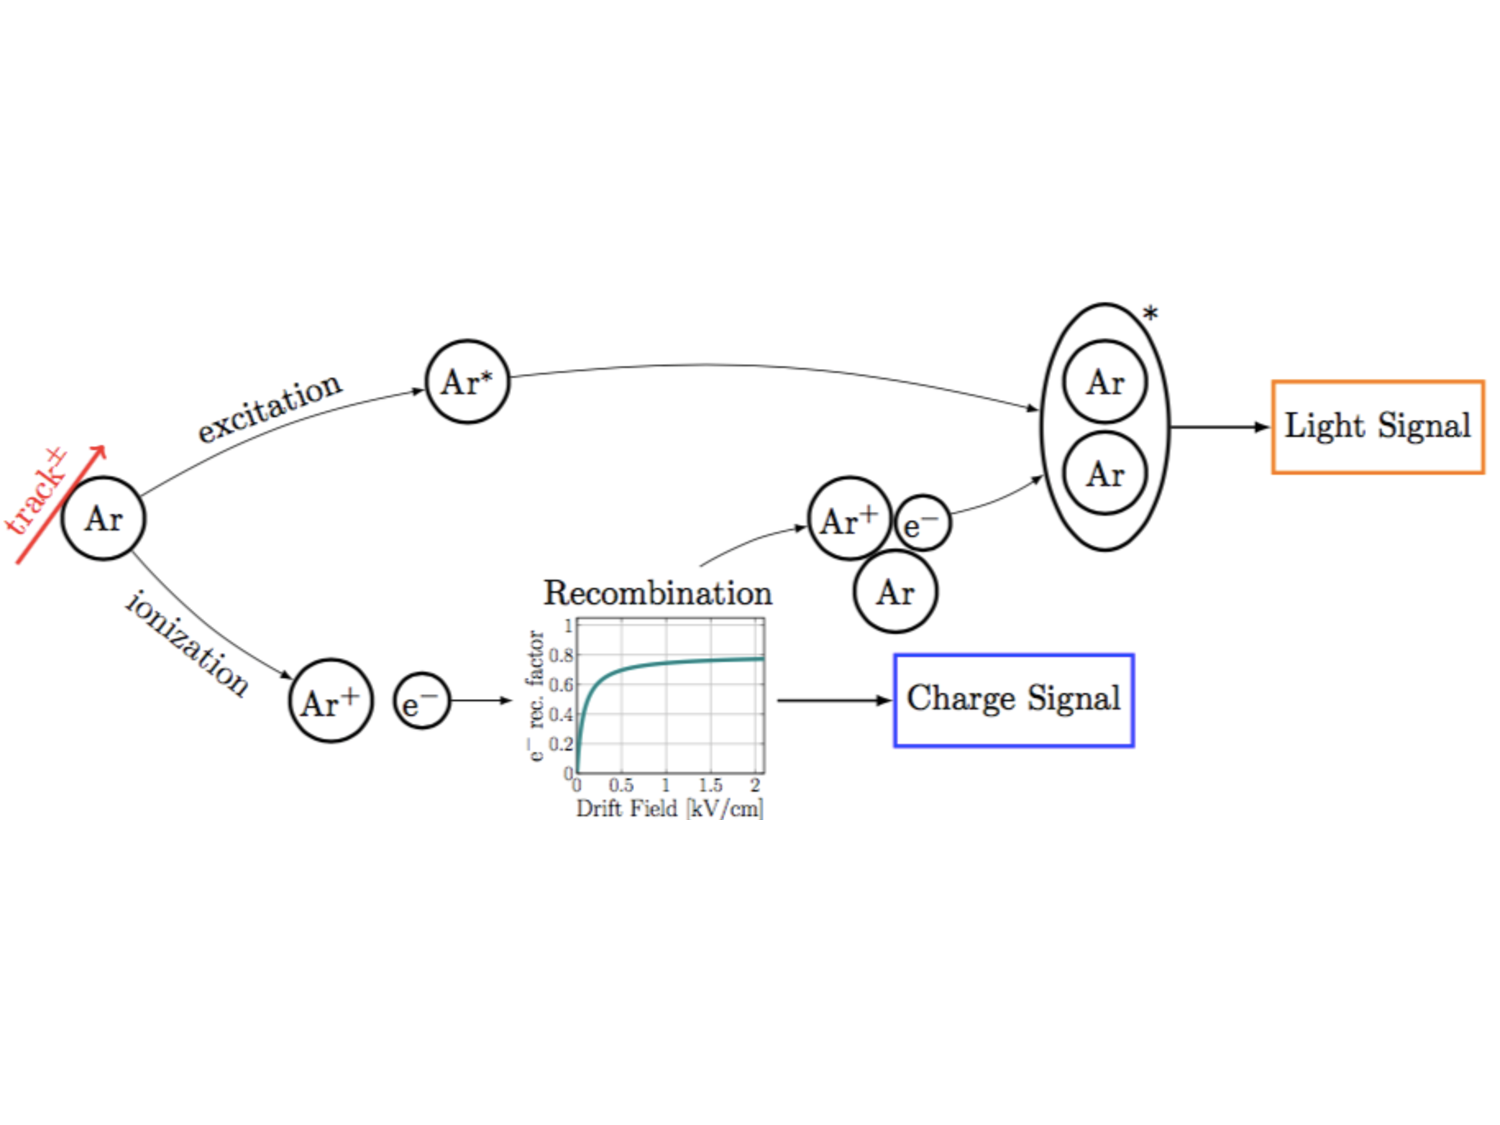
\includegraphics[width=0.95\textwidth]{dppd_6_0}
\end{dunefigure}

The secondary scintillation in the argon gas (i.e., the vapor phase) is unique to the \dpmod technology. It is the luminescence in gas caused by accelerated electrons in the \efield and in the \dword{lem} anode through Townsend amplification. The S2 signal provides information on the drift time and amount of ionization charge, thus supplementing information from the charge readout on the anode plane. For a given argon gas density, the number of S2 photons is proportional to the number of electrons, the \efield, and the length of the drift path in gas covered by the electrons. In an extraction field of \SI{3.0}{kV/cm} in gas, one electron generates about \num{100} downward-moving photons that cross the liquid argon surface \cite{Lux:2018zwd}. The time scale of S2 reflects the extraction time of original ionization from the liquid phase into the gas phase. Therefore, for about \SI{0.5}{kV/cm} drift \efield, this time scale is of the order of hundreds of microseconds. The time between the occurrence of the primary scintillation light and the secondary scintillation light is equivalent to the drift time of the electrons from the ionization coordinate to the \lar surface. This provides an accurate determination of the drift time in the active volume and, hence, a correction tool for the electron attachment (and the associated energy measurement).  


%The chapter begins with an overview of the system in Section~\ref{sec:fddp-pd-1}. Section~\ref{sec:fddp-pd-2} describes the photosensors, namely \dwords{pmt} %tubes  
%and the related \dword{hv} system, wavelength shifters and light collectors. The mechanics associated with the \dwords{pmt} is described in Section~\ref{sec:fddp-pd-3}, and the readout electronics in~\ref{sec:fddp-pd-4}. Section~\ref{sec:fddp-pd-5} details the photon calibration system to monitor the \dword{pmt} gain and stability. Then, the \dword{pd} performance is described in Section~\ref{sec:fddp-pd-6}, and the operations in Section~\ref{sec:fddp-pd-7}. Interfaces with other subsystems are described in Section~\ref{sec:fddp-pd-8}. Section~\ref{sec:fddp-pd-9} includes the installation, integration and commissioning plans. The \dword{qc} procedures are outlined in Section~\ref{sec:fddp-pd-10}. The main safety issues to consider are specified in Section~\ref{sec:fddp-pd-11}. To finish, the management and organization is described in Section~\ref{sec:fddp-pd-12}.

%%%%%%%%%%%%%%%%%%%%%%%%%%%%%%%%%
\subsection{Detector Sub-systems and Layout}
\label{sec:dp-pds-overview_layout}

The baseline design of the light collection system calls for \SI{20.3}{cm} (\SI{8}{in}) diameter cryogenic \dwords{pmt} from Hamamatsu Photonics\footnote{Hamamatsu Photonics\texttrademark{}, \url{http://www.hamamatsu.com/resources/pdf/etd/LARGE_AREA_PMT_TPMH1286E.pdf}} (model R5912-MOD20) distributed uniformly on the floor (bottom) of the cryostat and electrically shielded from the bottom cathode plane. Other \dword{pmt} manufacturers being considered include Electron Tubes Limited~\footnote{Electron Tubes Ltd\texttrademark{}, \url{http://www.electron-tubes.co.uk//}} and HZC~\footnote{HZC Photonics\texttrademark{}, \url{http://hzcphotonics.com/en_index.html}.}. According to the baseline design, \dpnumpmtch \dwords{pmt}, approximately \num{1} per \si{m$^2$}, will be installed. The outline of the \dword{dpmod} is shown in Figure~\ref{fig:dppd_3_1}.

\begin{dunefigure}[The \dword{dpmod} (partly open)]{fig:dppd_3_1}
{The \dword{dpmod} (partly open) with cathode, \dwords{pmt}, \dword{fc}, and anode plane with chimneys.}
%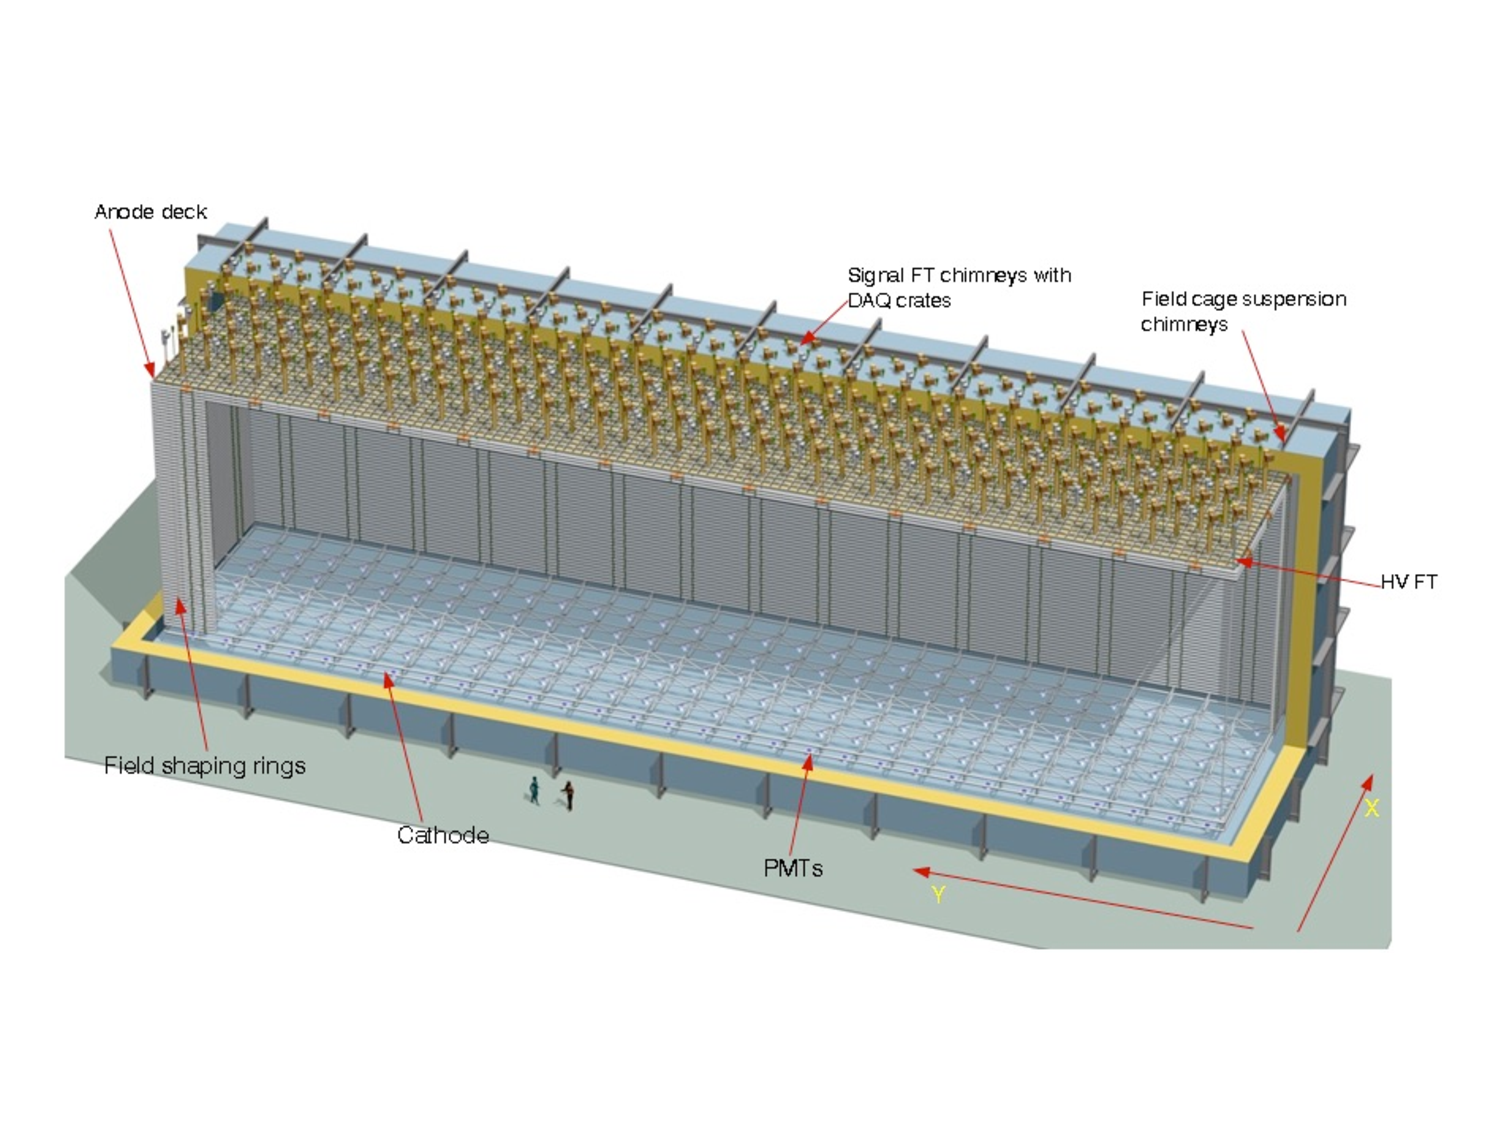
\includegraphics[width=0.95\textwidth]{dppd_3_1}
%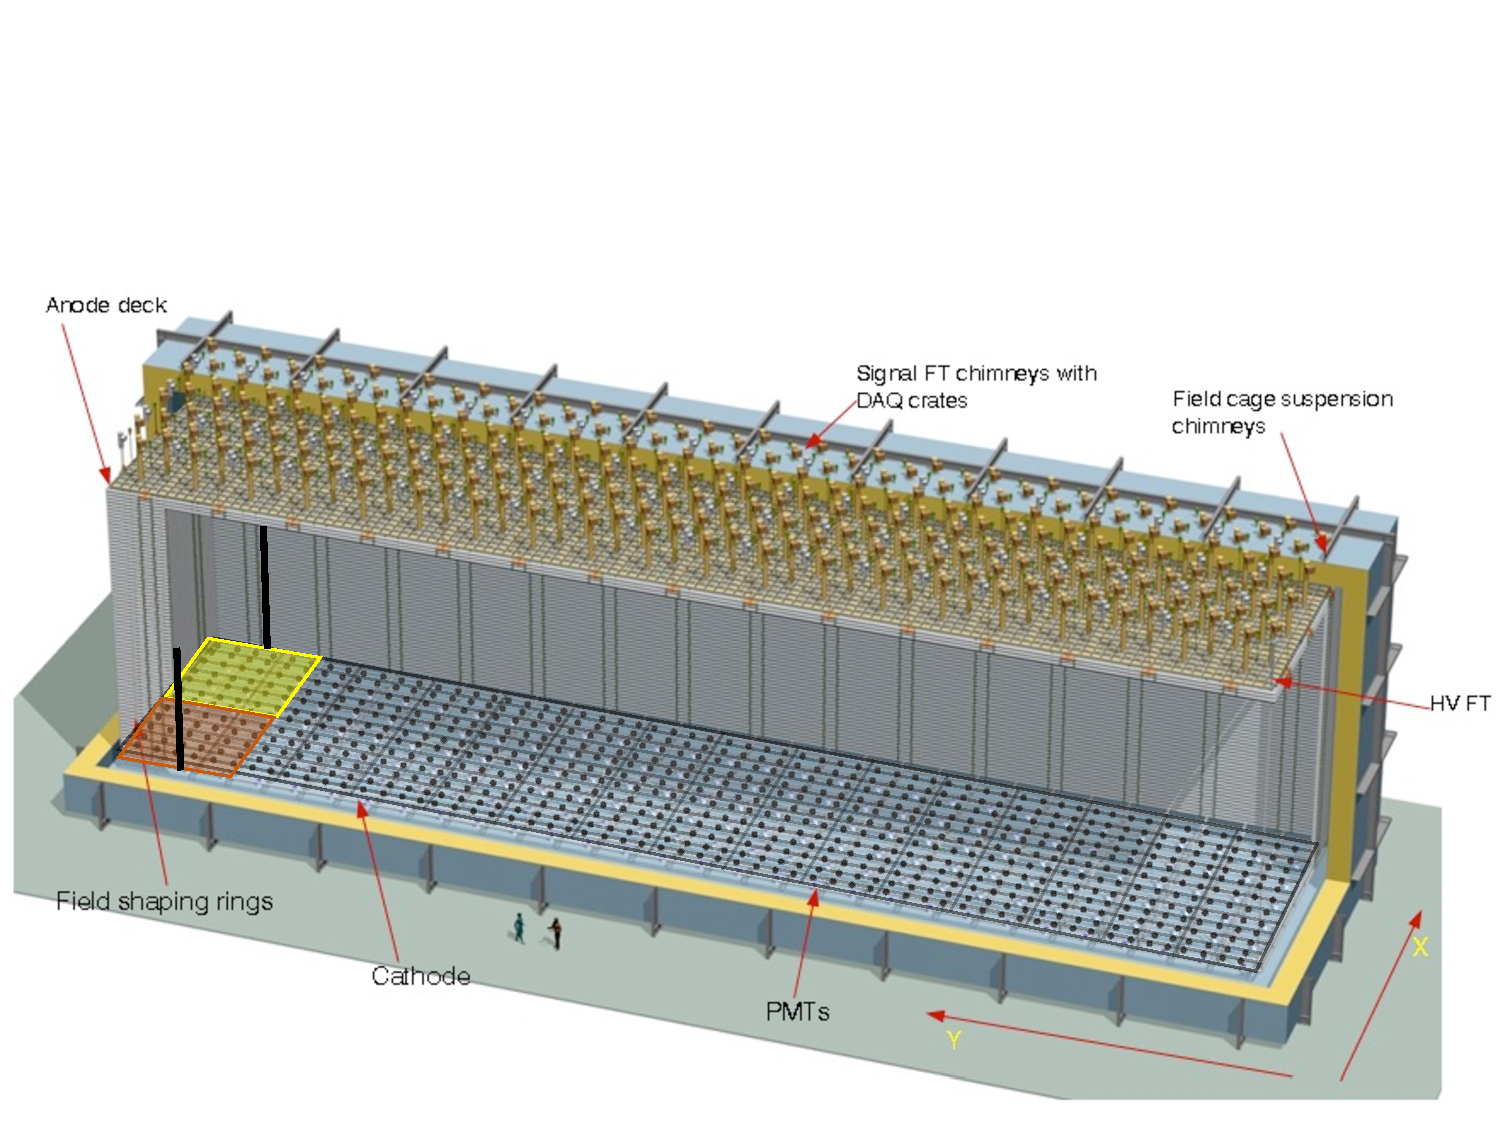
\includegraphics[width=0.95\textwidth]{dppd_1_1_v2}
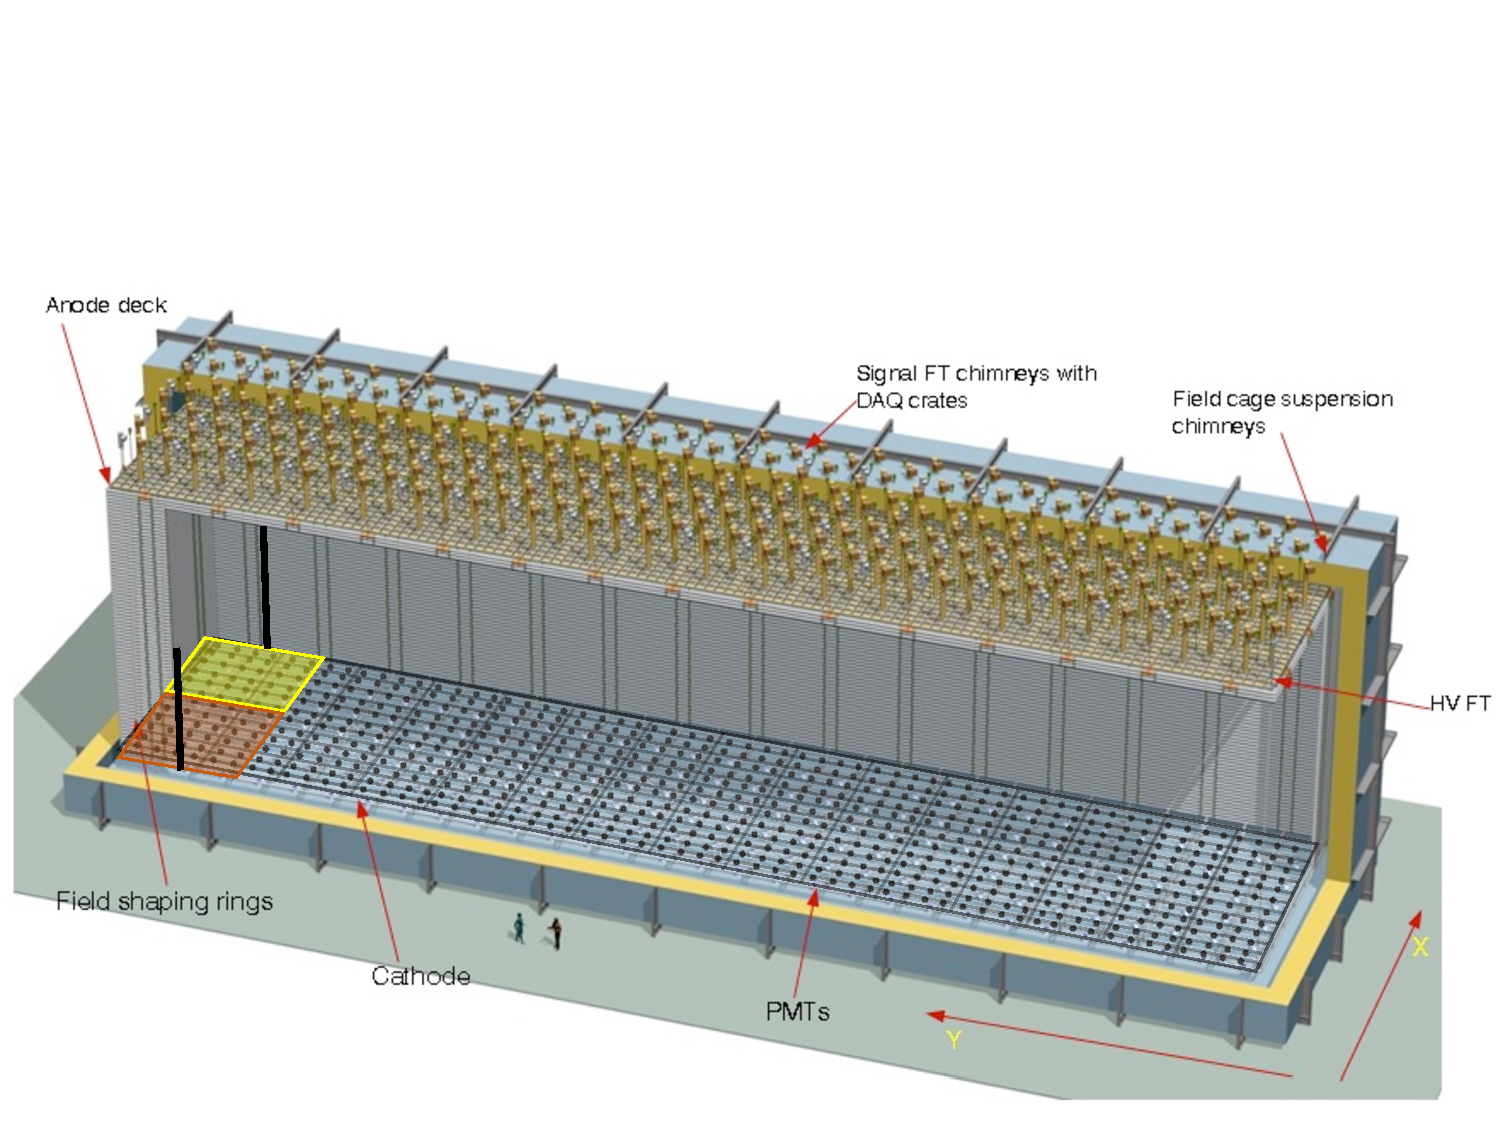
\includegraphics[width=0.95\textwidth]{dppd_1_1_v3}
\end{dunefigure}

The \dwords{pmt} are individually powered to %values 
positive high voltages between \num{1.5} to \num{2.0} \si{\kV} to separately adjust the \dword{pmt} gains. The Hamamatsu R5912 \dwords{pmt} are not sensitive to the \SI{127}{nm} scintillation light, so a wavelength shifter is required. A thin layer of \dword{tpb}~\cite{tpb} coating is applied directly on the \dword{pmt} window by evaporation. Section~\ref{sec:dp-pds-photosensors} describes the photosensor system.

The \dpnumpmtch \dwords{pmt} are individually attached to the cryostat floor \SI{1.02}{m} apart in both directions, via a \dword{pmt} support structure that counteracts the \dword{pmt} buoyancy. In order to enhance the light collection and to improve the photon detector response uniformity throughout the entire \dword{tpc} active volume, \dword{tpb} coated reflector/\dword{wls} panels will be installed on the top half of the \dword{fc} inner surfaces. Considering the linear relationship between the number of \dwords{pmt} and the detected light yield, and the mild dependence of the \dword{pds} physics performance on light yield and channel granularity, the optimization process that resulted in this baseline design can be considered very robust. The mechanical aspects of the \dword{pmt} support structures and the reflector/\dword{wls} assemblies are described in Section~\ref{sec:dp-pds-mechanics}.

The front-end \dword{pmt} base circuit for reading the photo-electron signals relies on a positive \dword{hv} supplied to the \dword{pmt} anode and on a grounded photo-cathode. A single cable for each \dword{pmt} carries both power and signal. \dword{hv} and signal splitters located outside the cryostat separate the fast \dword{pmt} response signal from the positive \dword{hv} with capacitive decoupling. The \dword{pds} readout electronics is described in Section~\ref{sec:dp-pds-electronics}.

A photon calibration system is required to determine the \dword{pmt} gain and to monitor the stability of the \dword{pmt} response. The LED-driven fiber calibration system of the \dword{pds} is described in Section~\ref{sec:dp-pds-calibration}. 

The basic unit of installation/operation is called a sector. The sectors are indicated as transparent red and yellow panels in Figure~\ref{fig:dppd_3_1}. One \dual \dword{pds} sector is \SI{6}{\m} $\times$ \SI{6}{\m} and houses \num{36} \dwords{pmt}. A total of \num{20} sectors will be installed in the detector. A single \dword{hv} cable per \dword{pmt} will be installed in the cryostat.
%The cables from the \dword{pmt} locations (RG303/U) will run in bundles at the cryostat floor to either side. The short cables attached to the \dword{pmt} bases will be connected to these long cables during the \dword{pmt} installation at the cryostat floor. The long cables from each sector will be bundled and will run through a cable tray along the \SI{12}{\m} side wall to the top of the cryostat. 
The cable trays for the two sectors in Figure~\ref{fig:dppd_3_1} are indicated as black vertical lines.
%The single cable density is approximately \SI{50}{\g/\m}. The cable length at the cryostat floor will be \SI{9}{\m} (determined by the farthest \dwords{pmt}), the side wall length is \SI{12}{\m}, and the additional average cable length per \dword{pmt} is estimated to be \SI{4}{\m}. Therefore, the overall cable length per \dword{pmt} is \SI{25}{\m}. This corresponds to approximately \SI{2}{\kg/\m} load on the cable trays on the side walls (a total of \SI{24}{\kg} assuming a cable density of \SI{50}{\g/\m}) per sector, also including the \num{6} calibration fibers. 

The high voltage cables will penetrate a feedthrough flange and end with SHV connectors, with the calibration fibers also penetrating a feedthrough flange and end with SMA connectors. One DN250 flange is used per sector of \dual \dword{pds}. One flange will house \num{36} SHV and \num{6} SMA connections. The \dual \dword{pds} design will have \num{20} penetrations on the cryostat roof, one per sector. 

The high voltage and signal crates will be at a density of one per sector for a total of \num{20} \dword{hv}/signal racks on the cryostat roof. Figure~\ref{fig:dppd_1_2} illustrates the layout of the feedthroughs and the \dword{hv}/signal/calibration racks for four sectors. The racks will contain the \dword{hv} crates, \dword{hv}/signal splitters, the \dword{utca} crates for the front-end electronics, and the calibration LED driver and the associated electronics for \num{36} \dwords{pmt}.

\begin{dunefigure}[The sketch of the cryostat roof layout for \dual PDS penetrations.]{fig:dppd_1_2}
{The sketch of the cryostat roof layout for \dual \dword{pds} penetrations.}
%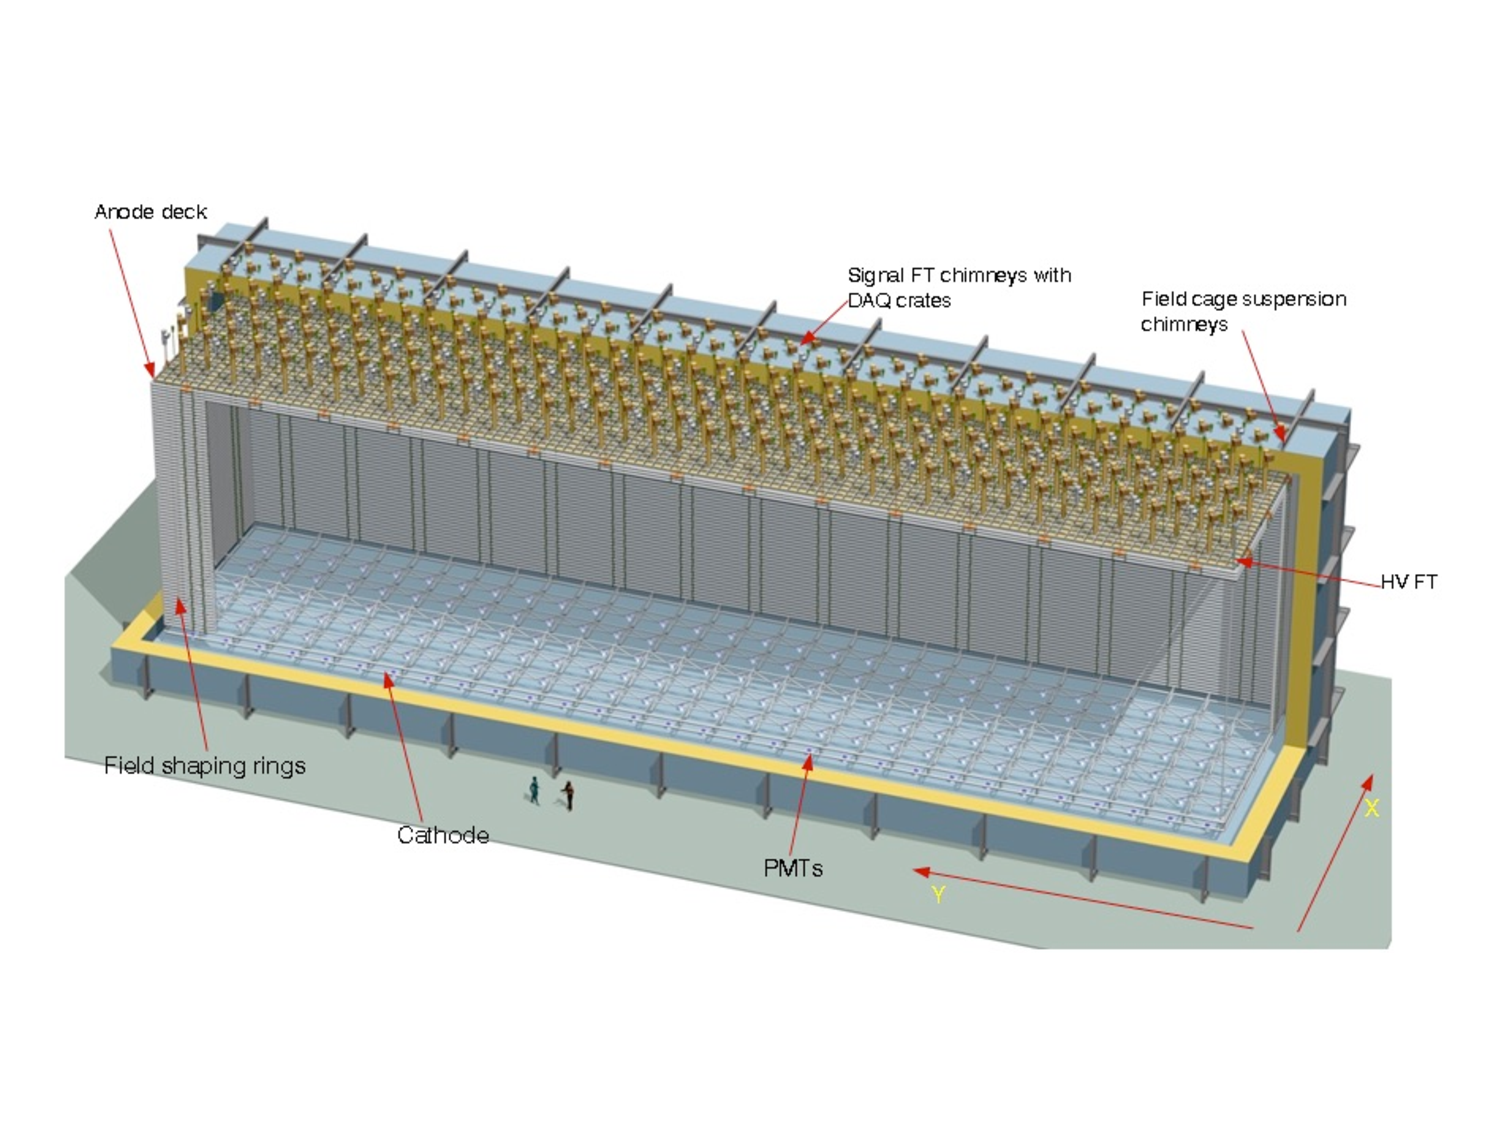
\includegraphics[width=0.95\textwidth]{dppd_3_1}
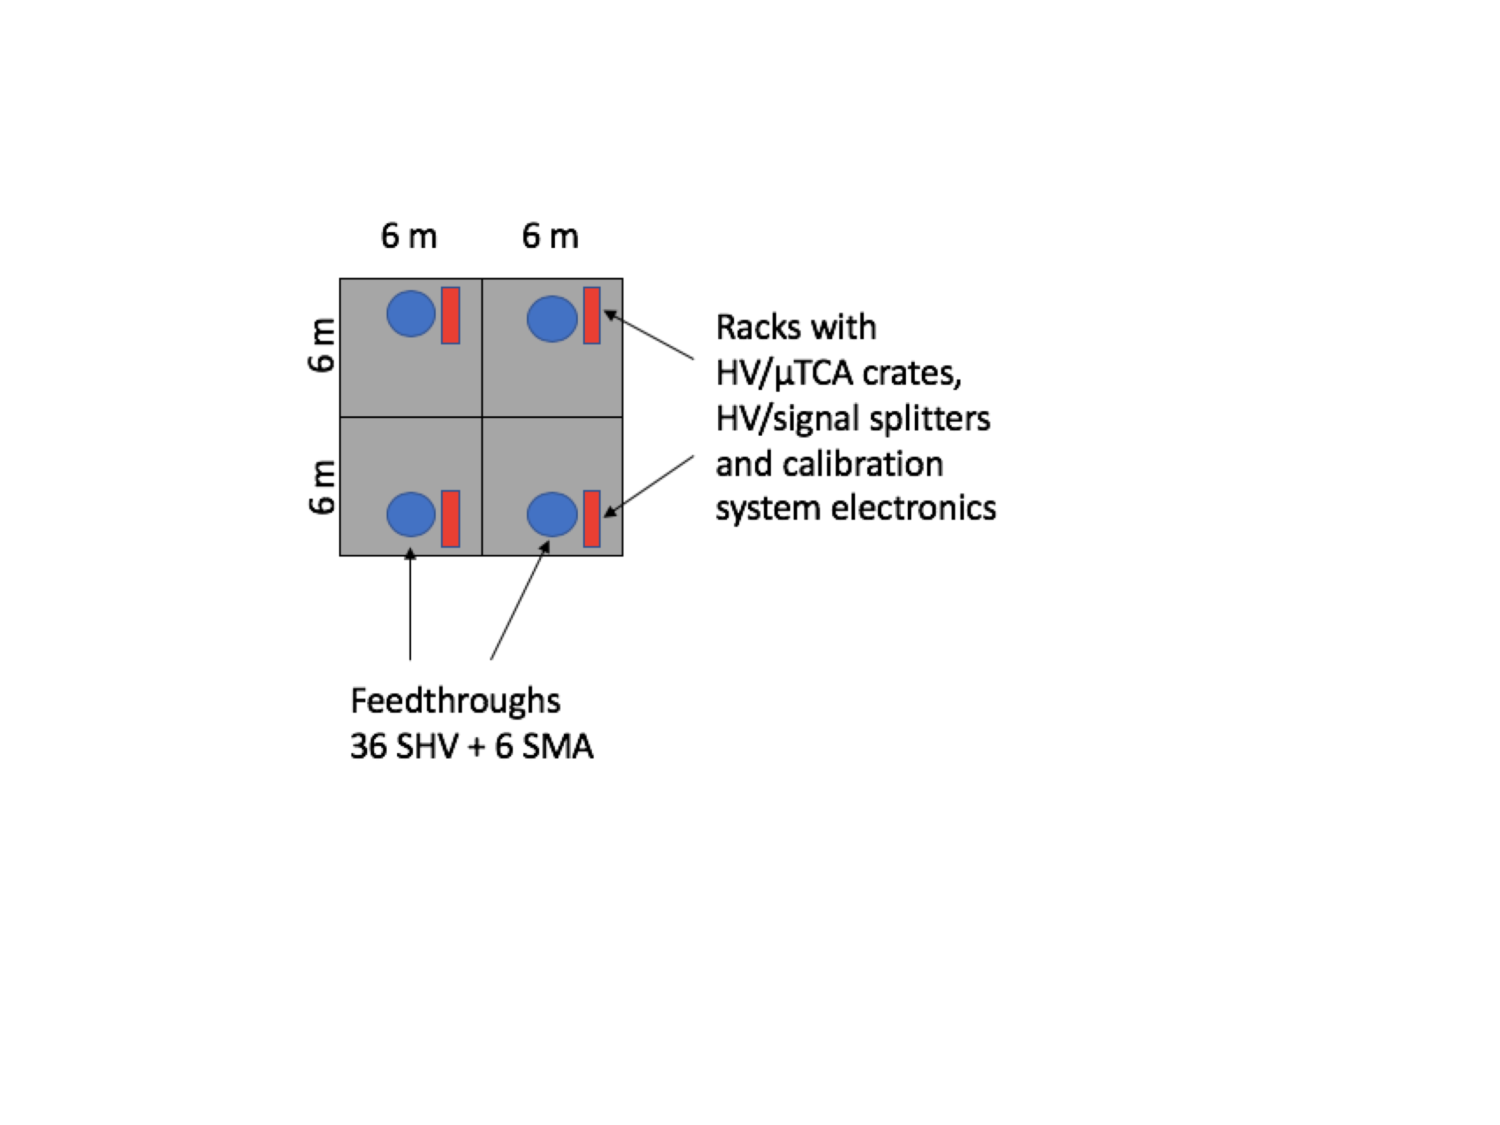
\includegraphics[width=0.55\textwidth]{dppd_1_2}
\end{dunefigure}

The cathode plane, described in Chapter~\ref{ch:dp-hv}, is placed approximately \SI{2}{m} above the bottom of the cryostat. Given the high dielectric constant of the \lar phase, the \dword{pmt} plane is a safe distance from the cathode plane. To protect the \dwords{pmt}, the ground grid is installed and placed at an identical potential as the \dword{pmt} photocathode (\SI{0}{V}).

%%%%%%%%%%%%%%%%%%%%%%%%%%%%%%%%%
\subsection{Operational Modes} %Principles}
\label{sec:dp-pds-oveerview_operation}

The physics program defines the operational modes of the \dual \dword{pds}. Measuring the neutrino oscillation parameters requires recording events upon receiving an external trigger from the beam, while non-beam physics such as \dwords{snb}, proton decay, or other rare events require special trigger conditions that include the \dword{pds}. Another operation mode is the \Dword{pmt} calibration run, which is initiated by the light calibration system with its dedicated hardware trigger.
%
Thus, the operation modes are
\begin{itemize}
\item External trigger: %this is mainly the case of 
A typical case is when the beam generates a hardware trigger (a beam gate);  it also includes software-generated triggers for test data.
\item Non-beam physics trigger: The electronics based on the \dword{pds} signals provides the trigger for, among other events, \dword{snb} and proton decay events;
\item Calibration trigger: The trigger is provided by the light calibration system during \dword{pds} calibrations.
\end{itemize}

The external and non-beam physics triggers run in parallel to ensure that rare events like \dwords{snb} are recorded efficiently. 

%%%%%%%%%%%%%%%%%%%%%%%%%%%%%%%%%
\subsection{Detector Design Specifications}
\label{sec:dp-pds-overview_specs}

The \dual \dword{pds} detector specifications are given in Table~\ref{tab:specs:just:DP-PDS}. The physics-driven rationale for each detector specification, and the means to validate them, are also summarized in the table. Validation of the detector specifications uses data from \dword{pds} prototypes (Section~\ref{sec:dp-pds-prototypes}) and from a full simulation/reconstruction of signal and background optical flashes in the \dpmod (Section~\ref{sec:dp-pds-performance}). 

%\fixme{(from Anne) Here is your requirements table. For SP, we've asked each chapter to include the "top 5" of the FD specs. That may not be appropriate for DP, since those top-level specs (approved by EB) may not exist yet.}

%% This file is generated, any edits may be lost.

\begin{longtable}{p{0.14\textwidth}p{0.13\textwidth}p{0.18\textwidth}p{0.22\textwidth}p{0.20\textwidth}}
\caption{Specifications for DP-PDS \fixmehl{ref \texttt{tab:spec:DP-PDS}}} \\
  \rowcolor{dunesky}
       Label & Description  & Specification \newline (Goal) & Rationale & Validation \\  \colhline

   \newtag{SP-FD-1}{ spec:min-drift-field }  & Minimum drift field  &  $>$\,\SI{250}{ V/cm} \newline ( $>\,\SI{500}{ V/cm}$ ) &  Lessens impacts of $e^-$-Ar recombination, $e^-$ lifetime, $e^-$ diffusion and space charge. &  ProtoDUNE \\ \colhline
    
   
  \newtag{SP-FD-2}{ spec:system-noise }  & System noise  &  $<\,\SI{1000}\,e^-$ &  Provides $>$5:1 S/N on induction planes for  pattern recognition and two-track separation. &  ProtoDUNE and simulation \\ \colhline
    
   
  \newtag{SP-FD-3}{ spec:light-yield }  & Light yield  &  $>\,\SI{20}{PE/MeV}$ (avg), $>\,\SI{0.5}{PE/MeV}$ (min) &  Gives PDS energy resolution comparable that of the TPC for 5-7 MeV SN $\nu$s, and allows tagging of $>\,\SI{99}{\%}$ of nucleon decay backgrounds with light at all points in detector. &  Supernova and nucleon decay events in the FD with full simulation and reconstruction. \\ \colhline
    
    \\ \rowcolor{dunesky} \newtag{SP-FD-4}{ spec:time-resolution-pds } & Name: Time resolution \\
    Description & The time resolution of the photon detection system shall be less than 1 microsecond in order to assign a unique event time.   \\  \colhline
    Specification (Goal) &  $<\,\SI{1}{\micro\second}$  ( $<\,\SI{100}{\nano\second}$ ) \\   \colhline
    Rationale &   Enables \SI{1}{mm} position resolution for \SI{10}{MeV} SNB candidate events for instantaneous rate $<\,\SI{1}{m^{-3}ms^{-1}}$.  \\ \colhline
    Validation &   \\
   \colhline

   \newtag{SP-FD-5}{ spec:lar-purity }  & Liquid argon purity  &  $<$\,\SI{100}{ppt} \newline ($<\,\SI{30}{ppt}$) &  Provides $>$5:1 S/N on induction planes for  pattern recognition and two-track separation. &  Purity monitors and cosmic ray tracks \\ \colhline
    

   
  \newtag{DP-PDS-1}{ spec:hit-relative-timing }  & Relative timing accuracy among hits  &  $<\,\SI{100}{ns RMS}$ &  Enable effective clustering of \dword{pmt} signals based on relative hit timing information. &  Full sim/reco of \dword{ndk}, \dword{snb} $\nu$ and radiological events. \\ \colhline
    
   
  \newtag{DP-PDS-2}{ spec:hit-snr }  & Hit signal-to-noise ratio  &  $>\,\num{5}$ &  Efficiently reconstruct single-\phel hits while rate of electronics noise hits remains manageable. &  Single-\phel and baseline noise \dword{rms} measurements in $3\times1\times1$ prototype. \\ \colhline
    
   
  \newtag{DP-PDS-3}{ spec:hit-relative-timing }  & Relative timing accuracy among hits  &  $<\,\SI{100}{ns RMS}$ &  Enable effective clustering of PMT signals based on relative hit timing information. &  Full simulation/reconstruction of NDK, SN $\nu$ and radiological events. \\ \colhline
    
   
  \newtag{DP-PDS-4}{ spec:hit-relative-timing }  & Relative timing accuracy among hits  &  $<\,\SI{100}{ns RMS}$ &  Enable effective clustering of \dword{pmt} signals based on relative hit timing information. &  Full sim/reco of \dword{ndk}, \dword{snb} $\nu$ and radiological events. \\ \colhline
    
   
  \newtag{DP-PDS-5}{ spec:pmt-dark-rate }  & PMT dark count rate  &  $<\,\SI{100}{kHz}$ &  Dark counts should have negligible effect on clustering algorithm and PDS-based calorimetry. &  Characterization of PMTs at cryogenic temperatures prior to installation. \\ \colhline
    
   
  \newtag{DP-PDS-6}{ spec:pds-dynamic-range }  & Dynamic range per channel  &  $>\,\SI{200}{PE}$ &  Avoid hit saturation for energy depositions near cathode plane.  &  Full simulation/reconstruction of beam $\nu$ interactions near cathode plane.  \\ \colhline
    
   \newtag{DP-PDS-7}{ spec:time-resolution-dp-pds }  & Time resolution  &  $<\,\SI{1}{\micro\second}$ \newline ( $<\,\SI{100}{\nano\second}$ ) &  Enables \SI{1}{mm} position resolution for \SI{10}{MeV} SNB candidate events for instantaneous rate $<\,\SI{1}{m^{-3}ms^{-1}}$. &   \\ \colhline
    


\label{tab:specs:DP-PDS}
\end{longtable}

%\fixme{The next table is just the DP PDS. It doesn't include the two SP FD requirements you selected (3 and 15 I think).}
% This file is generated, any edits may be lost.
\begin{footnotesize}
%\begin{longtable}{p{0.14\textwidth}p{0.13\textwidth}p{0.18\textwidth}p{0.22\textwidth}p{0.20\textwidth}}
\begin{longtable}{P{0.12\textwidth}P{0.18\textwidth}P{0.17\textwidth}P{0.25\textwidth}P{0.16\textwidth}}
\caption{Specifications for DP-PDS \fixmehl{ref \texttt{tab:spec:DP-PDS}}} \\
  \rowcolor{dunesky}
       Label & Description  & Specification \newline (Goal) & Rationale & Validation \\  \colhline

   
  \newtag{DP-PDS-1}{ spec:hit-relative-timing }  & Relative timing accuracy among hits  &  $<\,\SI{100}{ns RMS}$ &  Enable effective clustering of \dword{pmt} signals based on relative hit timing information. &  Full sim/reco of \dword{ndk}, \dword{snb} $\nu$ and radiological events. \\ \colhline
     % 1
   
  \newtag{DP-PDS-2}{ spec:hit-snr }  & Hit signal-to-noise ratio  &  $>\,\num{5}$ &  Efficiently reconstruct single-\phel hits while rate of electronics noise hits remains manageable. &  Single-\phel and baseline noise \dword{rms} measurements in $3\times1\times1$ prototype. \\ \colhline
     % 2
   
  \newtag{DP-PDS-3}{ spec:hit-relative-timing }  & Relative timing accuracy among hits  &  $<\,\SI{100}{ns RMS}$ &  Enable effective clustering of PMT signals based on relative hit timing information. &  Full simulation/reconstruction of NDK, SN $\nu$ and radiological events. \\ \colhline
     % 3
   
  \newtag{DP-PDS-4}{ spec:hit-relative-timing }  & Relative timing accuracy among hits  &  $<\,\SI{100}{ns RMS}$ &  Enable effective clustering of \dword{pmt} signals based on relative hit timing information. &  Full sim/reco of \dword{ndk}, \dword{snb} $\nu$ and radiological events. \\ \colhline
     % 4
   
  \newtag{DP-PDS-5}{ spec:pmt-dark-rate }  & PMT dark count rate  &  $<\,\SI{100}{kHz}$ &  Dark counts should have negligible effect on clustering algorithm and PDS-based calorimetry. &  Characterization of PMTs at cryogenic temperatures prior to installation. \\ \colhline
     % 5
   
  \newtag{DP-PDS-6}{ spec:pds-dynamic-range }  & Dynamic range per channel  &  $>\,\SI{200}{PE}$ &  Avoid hit saturation for energy depositions near cathode plane.  &  Full simulation/reconstruction of beam $\nu$ interactions near cathode plane.  \\ \colhline
     % 6
   \newtag{DP-PDS-7}{ spec:time-resolution-dp-pds }  & Time resolution  &  $<\,\SI{1}{\micro\second}$ \newline ( $<\,\SI{100}{\nano\second}$ ) &  Enables \SI{1}{mm} position resolution for \SI{10}{MeV} SNB candidate events for instantaneous rate $<\,\SI{1}{m^{-3}ms^{-1}}$. &   \\ \colhline
     % 7


\label{tab:specs:just:DP-PDS}
\end{longtable}
\end{footnotesize}

\section{Photosensor System}
\label{sec:dp-pds-photosensors}

The baseline photodetector for the light readout is the Hamamatsu R5912-MOD20 \dword{pmt}. This is the same model used in \dword{pddp}. The Hamamatsu R5912-MOD20, depicted in  Figure~\ref{fig:dppd_2_1}, is an 8-inch diameter, 14-stage, high gain \dword{pmt} (nominal gain of \num{e9}). The maximum quantum efficiency of the R5912-MOD20 \dword{pmt} is approximately \SI{20}{\%} at \SI{400}{\nano\m}. In addition, this \dword{pmt} was designed to work at cryogenic temperatures by adding a thin platinum layer between the photocathode and the borosilicate glass envelope to preserve the conductance of the photocathode at low temperatures. This particular \dword{pmt} has proved reliable in other cryogenic detectors. The same or similar \dwords{pmt} have successfully operated in other \lar experiments like MicroBooNE~\cite{microboone}, MiniCLEAN \cite{miniclean}, ArDM, ICARUS T600 \cite{icarus}, and \dword{pddp}~\cite{protoDUNDP-tdr}. Discussions with other manufacturers like Electron Tubes Limited (UK) \cite{electrontubeslim} and HZC (China) \cite{hzc} are on-going to include them in the program.

\begin{dunefigure}[Picture of the Hamamatsu R5912-MOD20 \dword{pmt}.]{fig:dppd_2_1}
{Picture of the Hamamatsu R5912-MOD20 \dword{pmt} \cite{hamamatsu-5912}.}
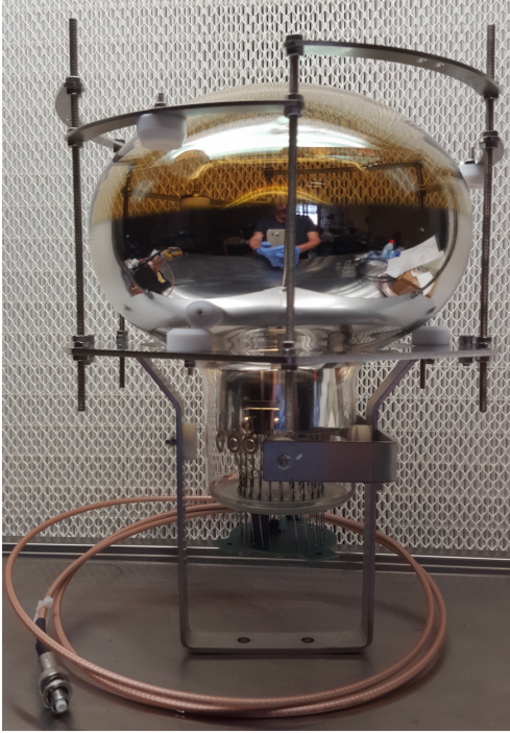
\includegraphics[width=0.3\textwidth]{dppd_2_1}
\end{dunefigure}

The baseline number of \dwords{pmt} is \dpnumpmtch with \num{80} spares.  Several operations and tests must be performed with the \dwords{pmt} before they are installed. The \dwords{pmt} must be ordered with sufficient lead time to complete the following planned operations: assembling the voltage divider circuit, mounting on the support structure, testing at room and cryogenic temperatures, packing and shipping to the \dword{ctsf}. The \dword{tpb} coating of the \dword{pmt} windows will be done at the \dword{ctsf}. The \dwords{pmt} will be re-tested for validation of basic functionality at the \dword{ctsf} and at \surf before installation (see Section~\ref{sec:dp-pds-installation}). Considering the large number of \dwords{pmt} required by \dual \dword{pds}, the purchase order must be completed at least two years before installation. A staged or staggered order with a steady supply of \dwords{pmt} would be most convenient and will be negotiated with the manufacturer.

%%%%%%%%%%%%%%%%%%%%%%%%%%%%%%%%%
\subsection{Photodetector Characterization}
\label{sec:dp-pds-selection-characterization}

Before installation, the most important characteristics of the \dword{pmt} response must be determined with two goals: to possibly reject under-performing \dwords{pmt} and to store the characterization information in a database for later use during the \dword{dpmod} commissioning and operation.

The basic and most important parameters to characterize are the dark count rate versus high voltage and the gain versus high voltage. Both parameters must be measured at room and cryogenic temperatures. As with the baseline \dword{pmt} model, the rates of pre-pulsing and after-pulsing should be negligible, but they will be measured as part of testing. 

From the mechanical point of view, the test set up requires a light-tight dark vessel filled with cryogenic liquid (argon or nitrogen) and an infrastructure for filling and operating the vessel with temperature and liquid-level controls. For \dword{pddp}, \num{10} \dwords{pmt} were tested at a time over a week because cryogenic tests of \dwords{pmt} require several days for \dword{pmt} thermalization \cite{Belver:2018erf}. Figure~\ref{fig:dppd_2_2a} shows the  \dword{pddp} \dwords{pmt} being installed in the testing vessel.
Increasing the capacity of the vessel, and thus the number of \dwords{pmt} that can be tested simultaneously,
could reduce the duration of the characterization test per \dword{pmt}.

\begin{dunefigure}[Picture of the \dwords{pmt} being installed in the testing vessel]{fig:dppd_2_2a}
{Picture of the \dwords{pmt} being installed in the testing vessel used for the \dword{pddp} \dwords{pmt}.}
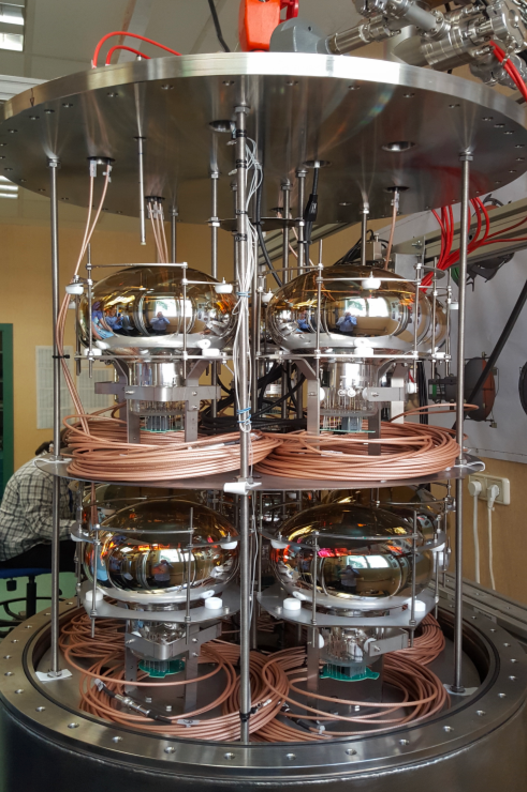
\includegraphics[width=0.3\textwidth]{dppd_2_2a}
\end{dunefigure}

Figure~\ref{fig:dppd_2_2b} shows a sketch of the proposed set up for \dword{pmt} characterization tests. For the electronics, the test set up requires an \dword{hv} power supply, a discriminator, a counter for the dark rate measurements, a pulsed light source, and a charge-to-digital or analog-to-digital converter for the \dword{pmt} gain versus voltage measurements. All instruments must allow computer control to automate data acquisition.

\begin{dunefigure}[Sketch of the set up for \dword{pmt} characterization tests.]{fig:dppd_2_2b}
{Sketch of the set up for \dword{pmt} characterization tests.}
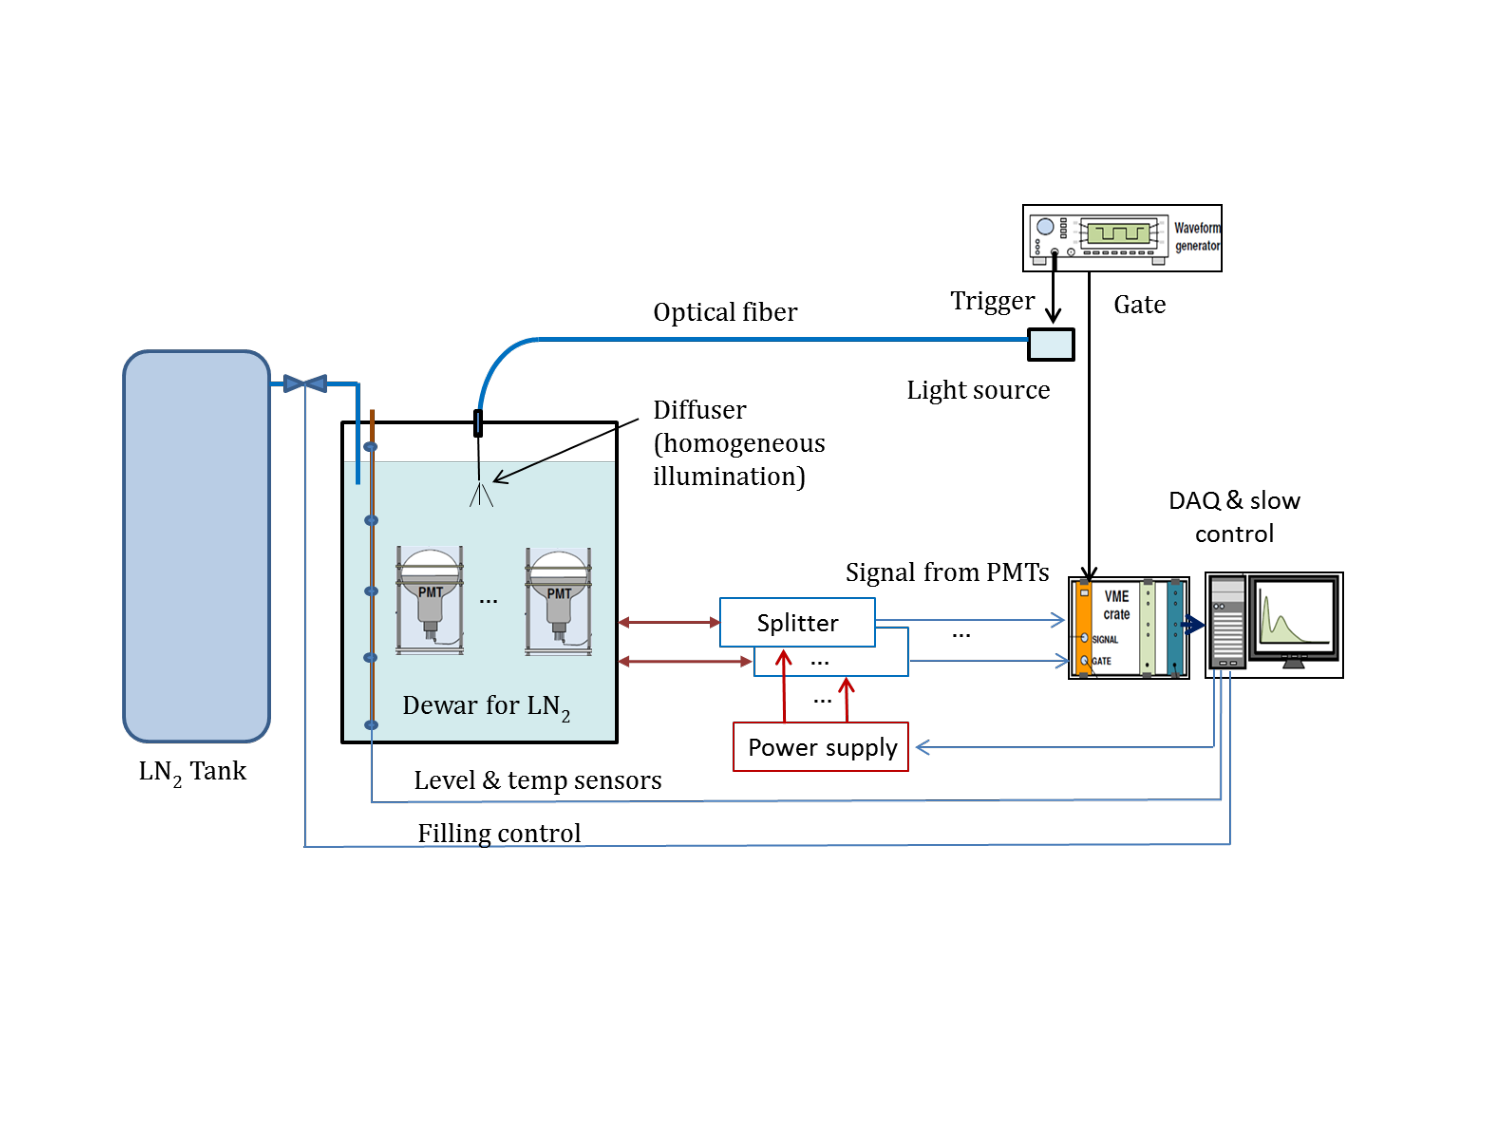
\includegraphics[width=0.7\textwidth]{dppd_2_2b}
\end{dunefigure}


%%%%%%%%%%%%%%%%%%%%%%%%%%%%%%%%%
\subsection{High Voltage System}
\label{sec:dp-pds-HV}

Based on the experience with the \dword{wa105} prototype, the A7030 power supply modules from CAEN~\footnote{CAEN\texttrademark{}, \url{http://www.caen.it/csite/CaenFlyer.jsp?parent=222}} are selected as the baseline power supply of the \dword{pmt} \dword{hv} system. 
These modules provide up to \SI{3}{kV} with a maximal output current of \SI{1}{mA} and a common floating ground to minimize noise. Module versions with \num{12}, \num{24}, \num{36}, or \num{48} \dword{hv} channels are available. The \dword{hv} polarity can be chosen for each module. Using the baseline \dword{pmt} powering scheme, modules with positive \dword{hv} polarity will be acquired for the experiment. Modules with \num{36} \dword{hv} channels and Radiall \num{52}\footnote{Radiall\texttrademark{}, \url{https://www.radiall.com/}.}  connectors are under consideration. The corresponding \dword{hv} cable connects the modules with the \dword{hv} splitters, described in Section~\ref{sec:fddp-pd-4.2}. For \dpnumpmtch \dwords{pmt}, \num{20} A7030 modules (+ \num{2} spares) are needed. These \num{20} \dword{hv} modules will be installed in mainframes from CAEN.

Each \dword{pmt} is powered individually.  This allows the gain of all \dwords{pmt} to be set individually by adjusting their operating high voltage.
This will be controlled by software. The software will interface to the \dword{pmt} calibration system and its database to extract the gain curves needed to set and/or equalize gains.

%%%%%%%%%%%%%%%%%%%%%%%%%%%%%%%%%
\subsection{Wavelength Shifting}
\label{sec:dppd-wls}

The \dual \dword{pds} requires wavelength-shifting of the \SI{127}{nm} scintillation photons toward visible wavelengths that can overlap with the photocathode luminous sensitivity. Coating the \dword{pmt} glass bulbs over the photocathode area with a thin film of \dword{tpb} has already been validated~\cite{Francini:2013lua} and is adopted as the baseline plan. 

\dword{tpb} is a wavelength shifter that has high efficiency for converting \lar scintillation \dword{vuv} light toward the light for which the \dword{pmt} photocathode is more sensitive. 

A thin layer of \dword{tpb} is deposited on the \dword{pmt} glass by means of a thermal evaporator that consists of a vacuum chamber with two copper crucibles (Knudsen cells) placed at the bottom of the chamber, see Figure~\ref{fig:dppd_11_4} in Section~\ref{sec:dp-pds-installation}. A \dword{pmt} is mounted on a rotating support that ensures a uniform coating layer and placed at the top of the evaporator with the  \dword{pmt} window pointing downward. The crucibles, filled with the \dword{tpb}, are heated to \SI{220}{\degreeCelsius}. At this temperature, the \dword{tpb} evaporates through a split in the crucible lid into the vacuum chamber, eventually reaching the \dword{pmt} window.

Several tests were performed to tune the evaporator's parameters, e.g., the coating thickness (\dword{tpb} surface density) and the deposition rate. A \dword{pmt} mock up covered with mylar foils was used for these tests. A \dword{tpb} surface density of \SI{0.2}{mg/cm^2}, the value for which the \dword{pmt} efficiency is stable as a function of the surface density, was chosen for \dword{pddp}. Efficiency measurements were performed by using a \dword{vuv} monochromator and by comparing the cathode current of a coated \dword{pmt} with the current value of a calibrated photodiode. From these efficiency tests, we concluded that approximately \SI{0.8}{g} of \dword{tpb} must be placed in the crucible for each evaporation to achieve the desired \dword{pmt} coating surface density. %The best deposition rate was fixed to about 6.5\,\AA/s. 
This value optimizes the quantity of \dword{tpb} used per evaporation while keeping the coating surface density fluctuations below \num{5}$\%$.  
Two to four \dwords{pmt}  with these specifications can be coated per day at a single coating station. 
Several coating stations will be required to keep the installation and testing schedule (see Section~\ref{sec:dp-pds-installation} for details). An average quantum efficiency of \SI{12}{\%} at \SI{127}{\nano\m} has been measured for TPB-coated \dwords{pmt} \cite{Bonesini:2018ubd}.

%We are considering, in coordination with the \dword{hvs} consortium, installing wavelength shifting films on the inner surfaces of the \dword{fc}. This would increase both light yield and response uniformity and is routinely used in \dual \lartpc{}s searching for dark matter, such as the ArDM~\cite{Boccone:2009zz} experiment. It is also under investigation for the \dword{spmod} concept, building on the experience of the \lariat experiment and the design for SBND. The same \dword{wls} compound used to coat the \dword{pmt} windows, \dword{tpb}, could be vacuum-evaporated on foils. The shifted longer wavelength light emitted by the foils would have a better chance to reach the \dword{pmt} windows than \SI{127}{nm} light because it has better reflective properties. 
 %
 %This concept would need to be demonstrated satisfactorily for performance and stability on the timescale of the experiment duration before it could become a part of the \dword{pds} system.

In order to enhance the light collection and to improve the photon detector response uniformity throughout the entire \dword{tpc} active volume, \dword{tpb} coated reflector/\dword{wls} panels will be installed on the \dword{fc} inner surfaces. The impact on the light yield and physics measurements was evaluated for two particular cases: The full coverage of the \dword{fc} inner walls with the panels and the coverage of only the upper half of the \dword{fc}. The conclusion from the simulation studies is that half coverage is sufficiently performant as shown in Fig. ~\ref{fig:dppd_fd_light_yield_comparisons}. In order to reduce the cost still keeping the \dword{pds} response uniformity, the baseline design is to equip only the top half of the \dword{fc} walls. The \dword{tpb} coating on the \dword{pmt} windows has \num{90} \% transmittance at \SI{425}{nm} (peak of the emission spectrum of \dword{tpb}) \cite{Francini:2013lua}, therefore the baseline design of the reflector/\dword{wls} panels is optimal. 

The reflector/\dword{wls} panel will be constructed with \SI{1}{\mm} thick \SI{93}{\cm} $\times$ \SI{93}{\cm} G10/FR4 plates. The central \SI{91}{\cm} (H) $\times$ \SI{93}{\cm} (W) area only on one side of the panel will be laminated with a reflective foil, which will then be evaporated with \dword{tpb}. The top and bottom \SI{1}{\cm} portion of the panel without coated foils will be sandwiched between horizontal support bars. Sketches of the panel are shown in Fig.~\ref{fig:dppd_reflective_panel}. The support structure of the panels is described in Section~\ref{sec:dp-pds-mechanics}. 
\begin{dunefigure}[Sketches of the front (left) and side (right) views of the reflective foil/\dword{wls} panel.]{fig:dppd_reflective_panel}
{Sketches of the front (left) and side (right) views of the reflector/\dword{wls} panel (not to scale).}
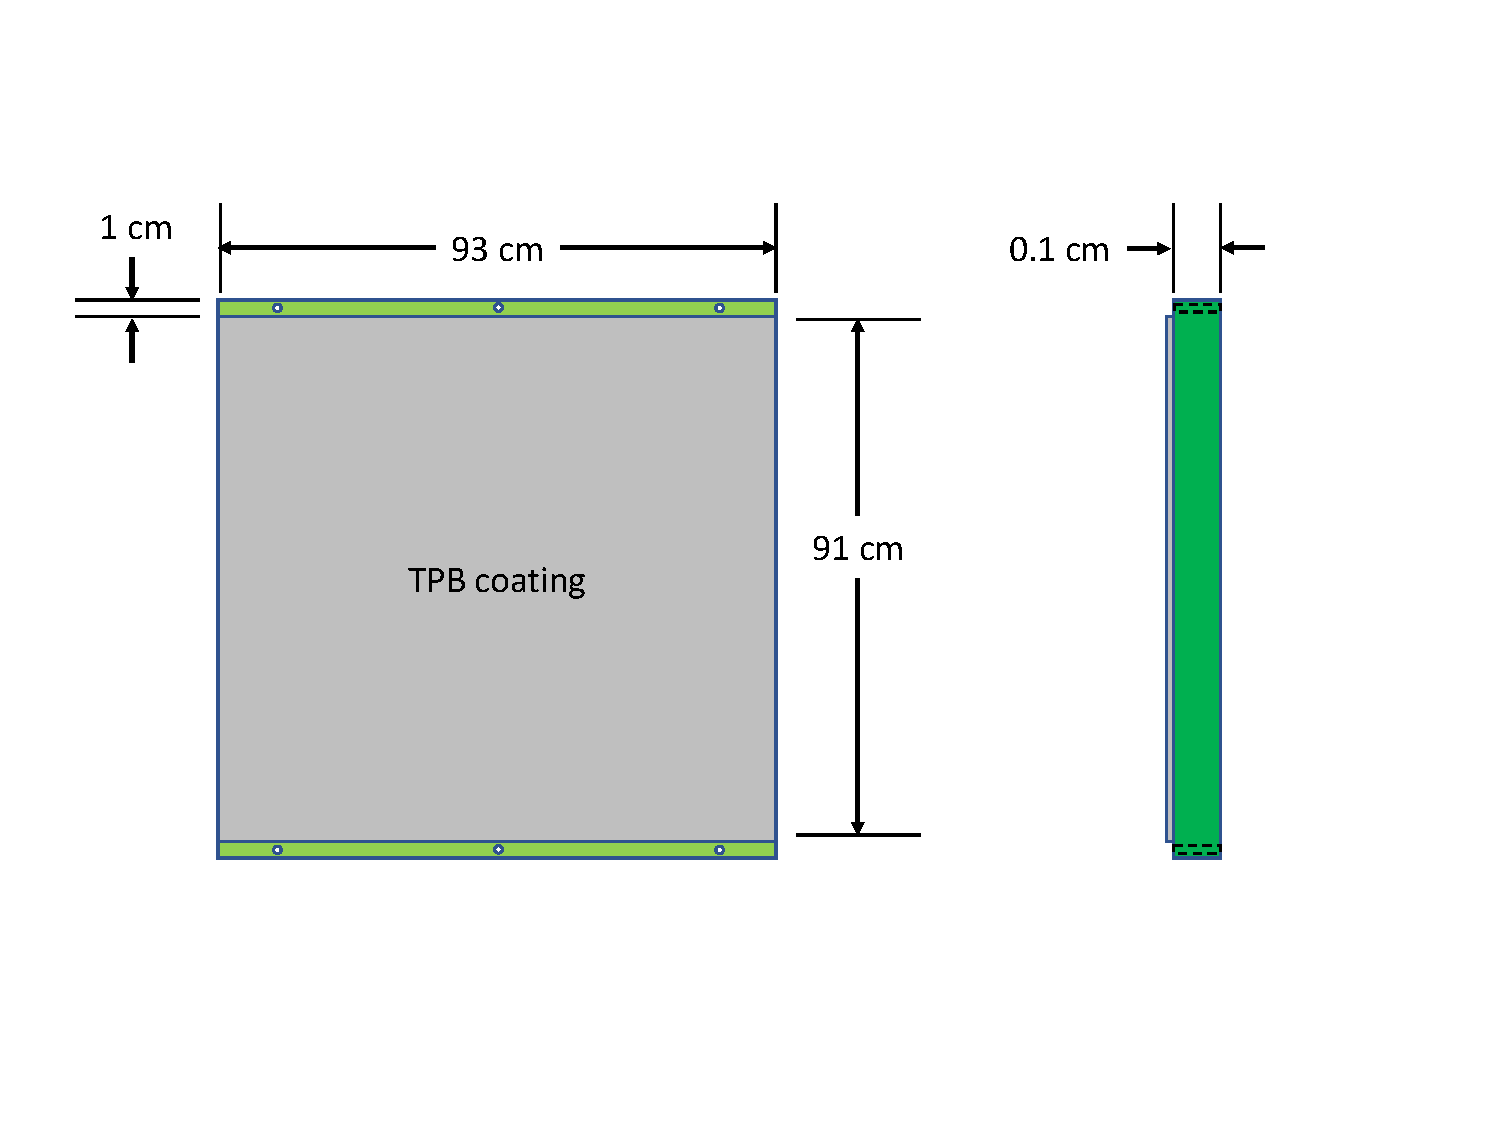
\includegraphics[width=0.7\textwidth]{dppd_reflective_panel}
\end{dunefigure}

\section{Mechanics}
\label{sec:dp-pds-mechanics}

\subsection{\dshort{pmt} Support Structure}
\label{subsec:dp-pds-mechanics-pmtsupport}

A uniform array of \dpnumpmtch cryogenic Hamamatsu R5912-MOD20 \dwords{pmt}, below the transparent cathode structure, will be fixed on the membrane floor in the areas between the membrane corrugations. The arrangement of the \dwords{pmt} accommodates the cryogenic piping on the membrane floor, and other elements installed in this area.

The mechanics for the attachment of the \dwords{pmt} were carefully studied. The \dword{pmt} buoyancy must be counteracted while avoiding stress to the \dword{pmt} glass due to differentials in the thermal contraction between the support and the \dword{pmt} itself. The attachment is done via a stainless steel support base point-glued to the membrane via four adhesive injection holes. The weight of the support and \dword{pmt} (approximately \SI{7}{\kg}) exceeds the buoyancy force of the system. Given the large standing surface of the stainless steel plate, these supports also ensure stability against possible lateral forces acting on the \dwords{pmt} due to the liquid flow. Figure \ref{fig:dppd_3_2} shows the \dword{pmt} with its support base attached to the bottom of the \dword{pddp} cryostat.


\begin{dunefigure}[Hamamatsu R5912-MOD20 PMT in ProtoDUNE-DP.]{fig:dppd_3_2}
{Picture of the cryogenic Hamamatsu R5912-MOD20 \dword{pmt} fixed on the membrane floor of \dword{pddp}. The optical fiber of the calibration system is also visible.}
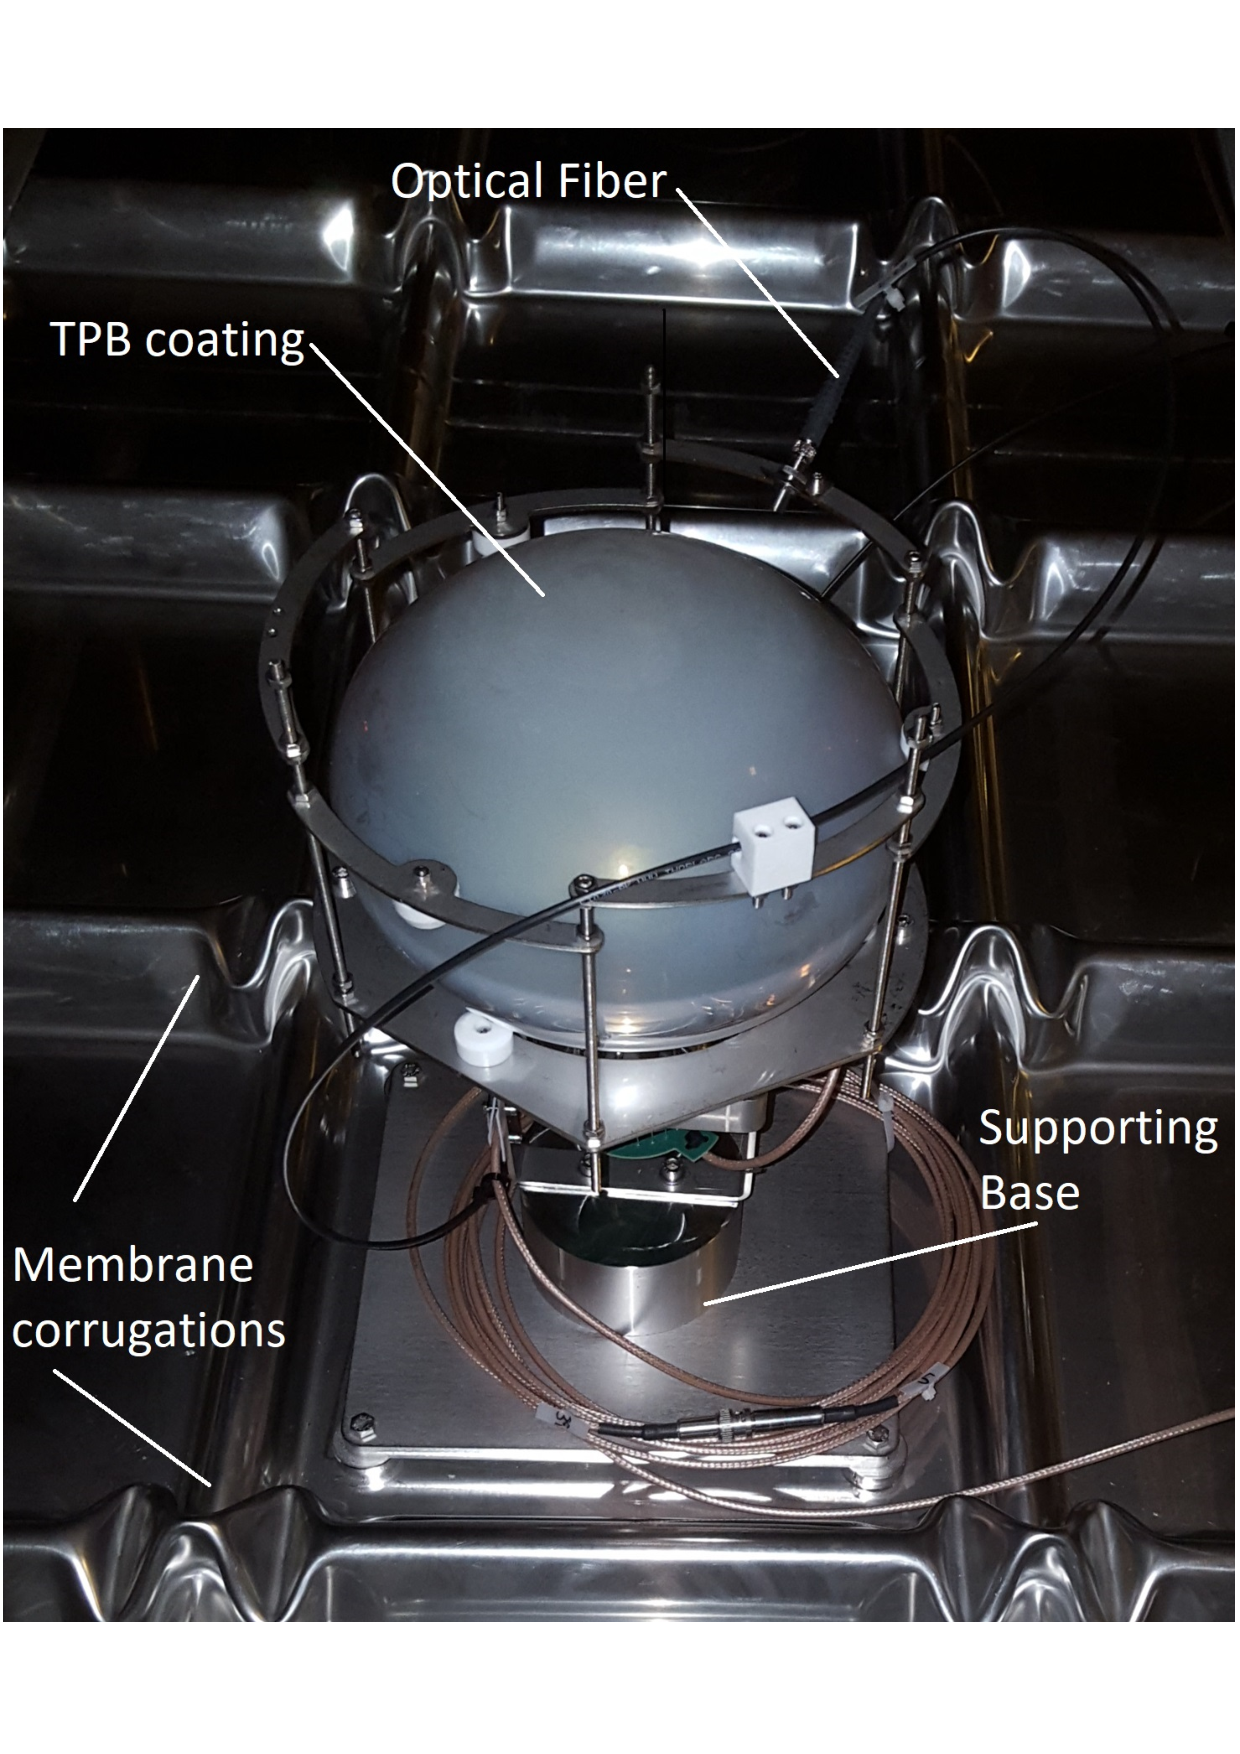
\includegraphics[width=0.42\textwidth]{dppd_3_n2}
\end{dunefigure}

%\fixme{Update Fig.~\ref{fig:dppd_3_2} of PMT support structure.}

%The \dword{hv} and \dual \dword{pds} consortia is studying an alternative to the table-like assembly of the ground grid: the concept of individual ground grids for each \dword{pmt}. In this option, the grids would be mechanically attached to the support structure. This will increase the acceptance of the \dwords{pmt} at larger angles.

The support frame structure mainly comprises \num{304}L stainless steel with some small Teflon (PTFE) pieces assembled by A4 stainless steel screws that minimize the mass while securing the \dword{pmt} support to the cryostat membrane. The design %was done taking 
takes into account the shrinking of the different materials during the cooling process to avoid breaking the \dword{pmt} glass.
Over-pressure tests were carried out for \dword{pddp}, and further tests ensure correct performance under pressure. An individual \dword{pmt} mount has been designed and tested in the  \dword{wa105} prototype~\cite{Zambelli:2017dkg}, and the same design is used for \dword{pddp}.

Installation of an individual ground grids mechanically attached to the \dword{pmt} support structures is also under consideration by the \dword{hv} and \dual \dword{pds} consortia (See Appendix~\ref{sec:dp-pds-appendix-grid}).

%%%%%%%%%%%%%%%%%%%%%%%%%%%%%%%%%%%%%%%%%%%%%%%%%%%%%%%%%%%%%%%%%%%

\subsection{Reflector/\dshort{wls} Panel Assemblies}
\label{subsec:dp-pds-mechanics-reflectors}

The reflector/\dword{wls} panels that will be mounted on the inner surface of the \dword{fc} will be \SI{1}{\mm} thick \SI{93}{\cm} $\times$ \SI{93}{\cm} G10/FR4 plates, with the central \SI{91}{\cm} (H) $\times$ \SI{93}{\cm} (W) area laminated with reflective foil, which is coated with \dword{tpb} (see Figure~\ref{fig:dppd_reflective_panel}). The panels will be supported by G10/FR4 support bars. Six horizontal bars of \SI{199}{\cm} (three at the front and three at the back), six vertical bars of \SI{186}{\cm} (all at the back) and four reflector/\dword{wls} panels will form a unit reflector/\dword{wls} panel assembly to be mounted on the \dword{fc}. The panels will be sandwiched between the horizontal support bars along the non-laminated edges. Six vertical bars will be placed on the side of the panels without the reflective coating, aligning the holes. The structure will then be assembled by placing \num{24} screws.

The horizontal support bars will be attached to the FRP I-beams of the \dword{fc}, which are spaced \SI{2}{\m} apart, by stainless steel screws. One end of the bar will be tightly screwed, while the other loosely to allow motion due to differential thermal contractions. Figure \ref{fig:dppd_reflective_panel_support} shows sketches of the horizontal support bars with one of the two screw holes elongated to allow the support bar movement on the mounting screw.

\begin{dunefigure}[Reflector/WLS panel assembly horizontal support bars.]{fig:dppd_reflective_panel_support}
{Sketches of the reflector/\dword{wls} panel assembly horizontal support bars (not to scale). (a) The top and bottom bars, (b) the middle bar, (c) the extended top and bottom bars to be mounted on the end submodules of the \dword{fc} super-modules, and (d) the special extended top and bottom bars to be mounted on the end submodules of the corner \dword{fc} side wall super-modules.}
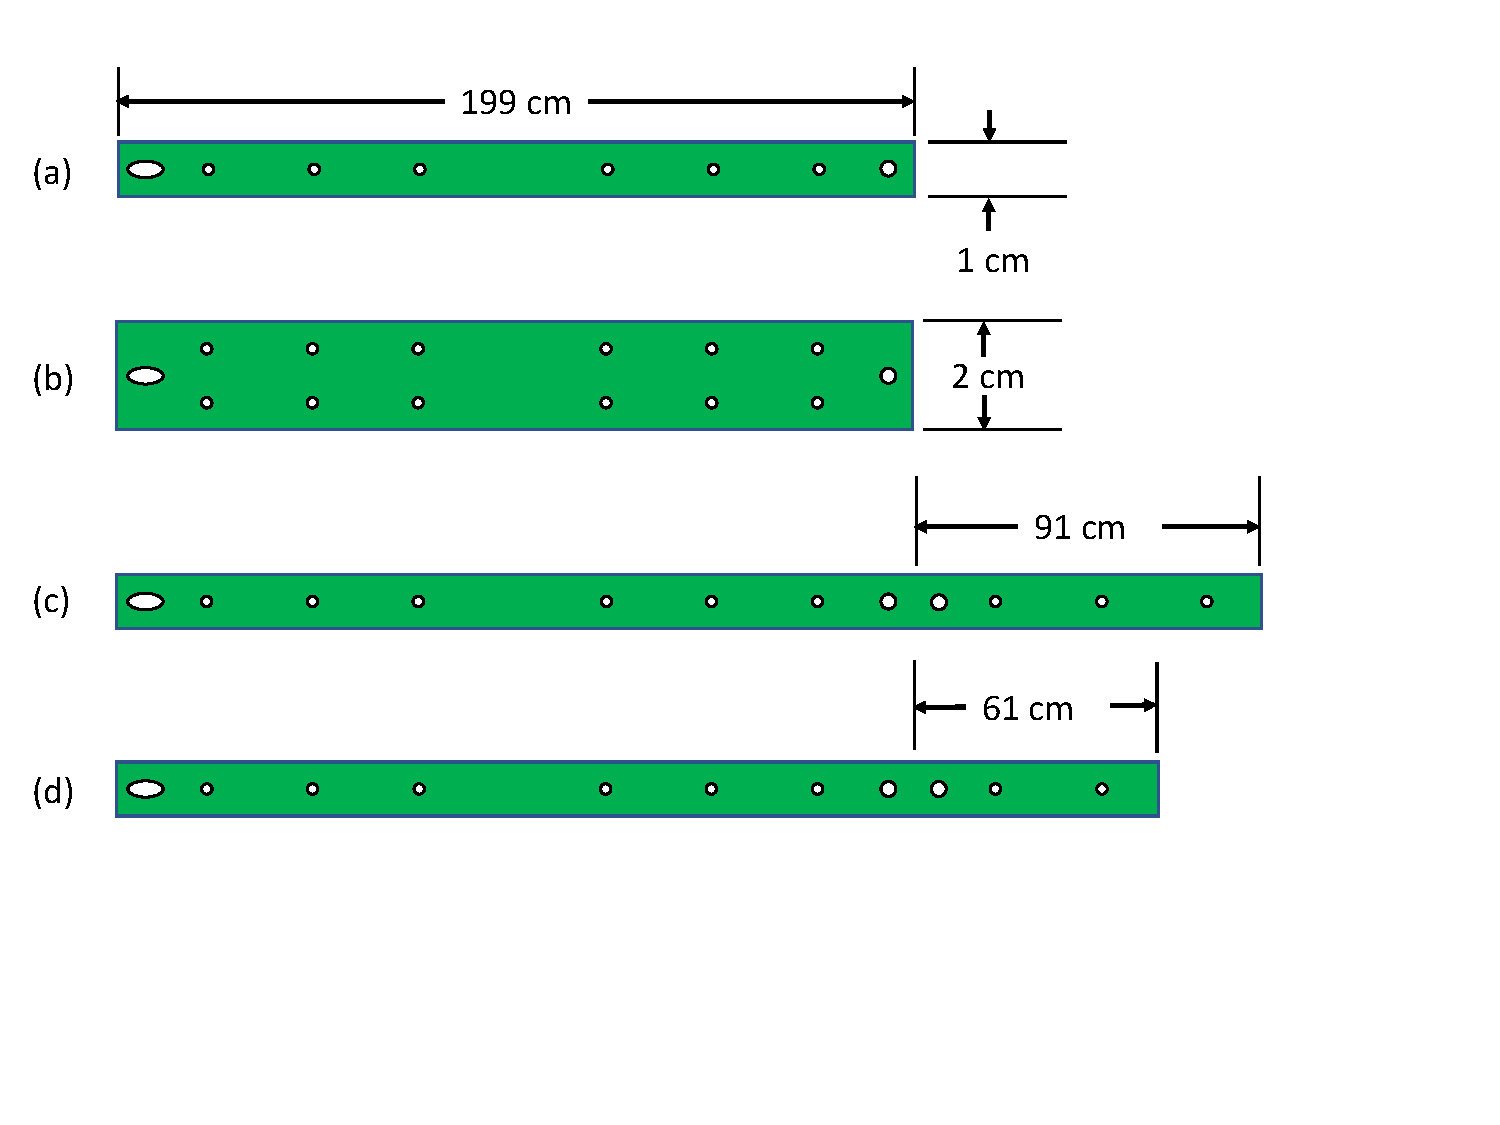
\includegraphics[width=0.65\textwidth]{dppd_reflective_panel_support}
\end{dunefigure}

The reflector/\dword{wls} panel assemblies at the inter-super-module areas will have extended structures: \SI{260}{\cm} (W) $\times$ \SI{186}{\cm} (H) for the corner side wall \dword{fc} sub-modules to accommodate the \num{2.4} degree tilt of the end walls, and \SI{290}{\cm} (W) $\times$ \SI{186}{\cm} (H) for all other \dword{fc} sub-modules at the intersection of two \dword{fc} super-modules. The extended assemblies will house \num{6} reflector/\dword{wls} panels, two of them in an extended part which is not supported at the end. Figure \ref{fig:dppd_reflective_panel_support} (c) shows the sketch of the support bar to be installed at the end submodules of the \dword{fc} super-modules except the end submodules of the corner \dword{fc} side wall super-modules of which the corresponding horizontal support bar is shown in Figure~\ref{fig:dppd_reflective_panel_support} (d). The special extended assemblies to be installed at the end submodules of the corner side wall super-modules will be \SI{30}{\cm} shorter than the regular extended assemblies to accommodate the approximately \SI{25}{\cm} approach of the end walls at middle drift distance (\SI{6}{\m}).

Figure \ref{fig:dppd_reflective_panel_onFC} shows inside (left) and outside (right) sketches of a unit reflector/\dword{wls} assembly. The blue bars are the I-beams of the \dword{fc}, the dark green bars are the horizontal and vertical support bars of the reflector/\dword{wls} panel assembly. The grey surfaces are the \dword{tpb} coatings on the panels. The vertical and horizontal gaps between the reflector/\dword{wls} panels allow liquid flow. 

\begin{dunefigure}[Inside and outside views of partial FC submodule with reflector/W:S panel assembly.]{fig:dppd_reflective_panel_onFC}
{Sketches of the inside with the reflective/\dword{wls} coating (left) and outside without the reflective/\dword{wls} coating (right) views of a partial \dword{fc} submodule with a reflector/\dword{wls} panel assembly. The blue bars are the FRP I-beams of the \dword{fc}. The dark green bars are the horizontal and vertical support bars. The grey surfaces are the \dword{tpb} coatings on the panels.}
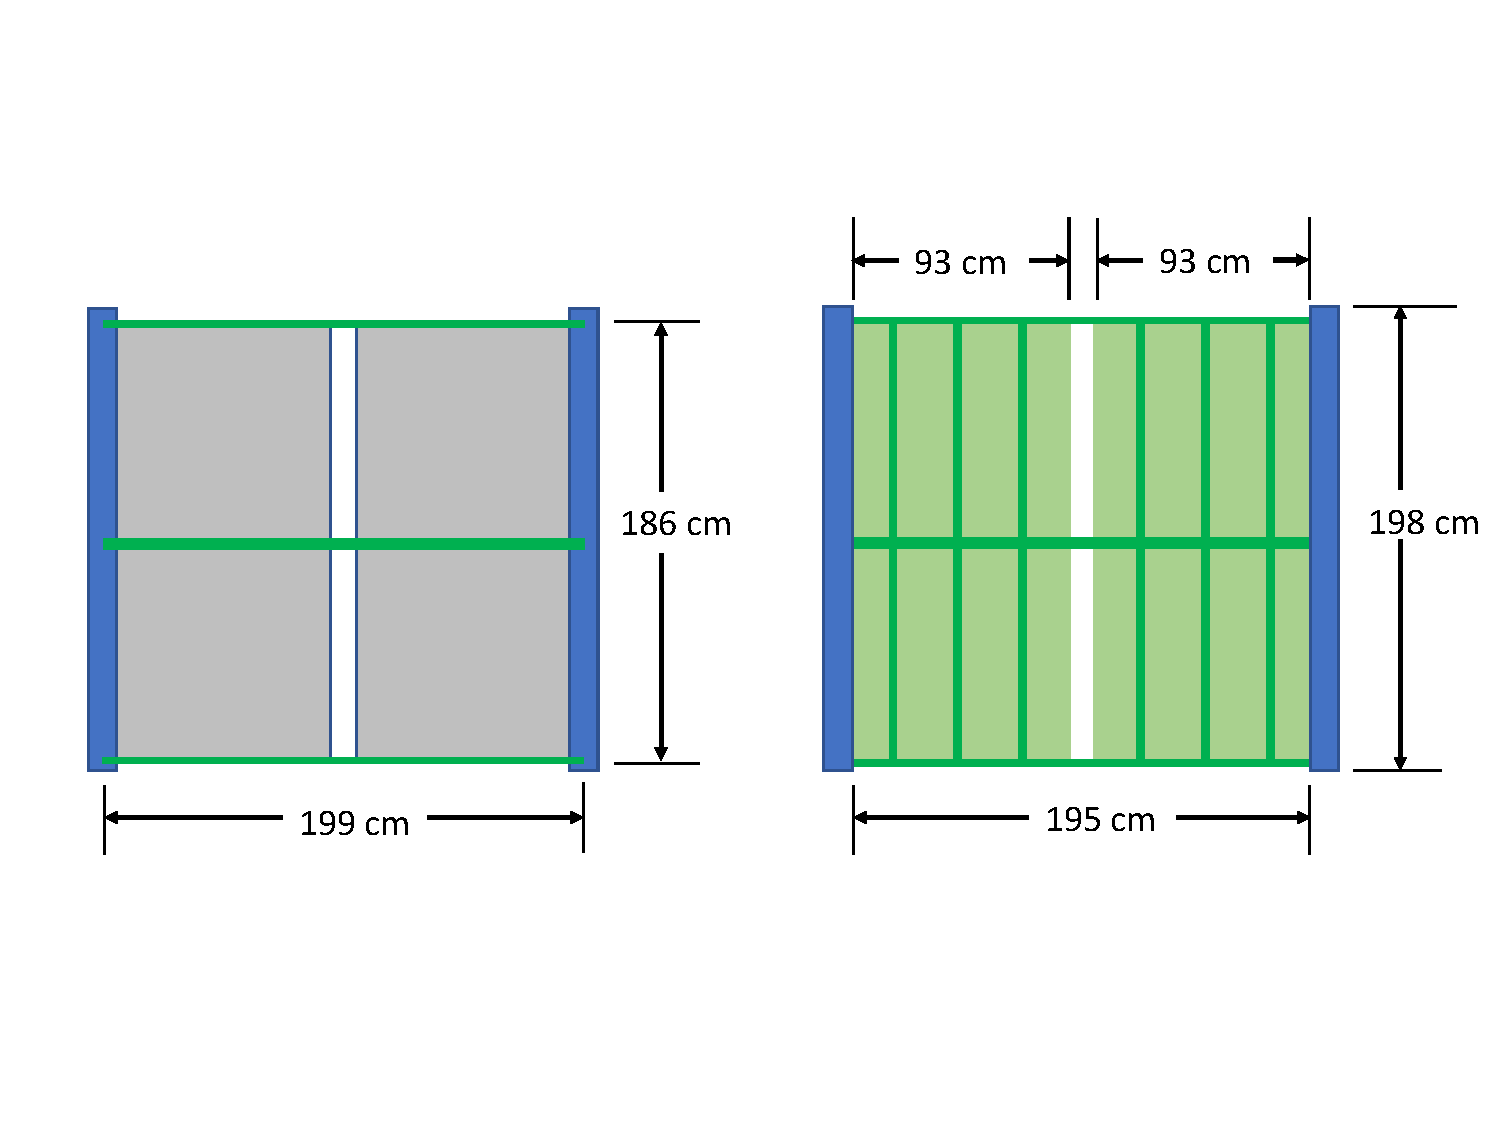
\includegraphics[width=0.8\textwidth]{dppd_reflective_panel_onFC}
\end{dunefigure}
\section{Readout Electronics}
\label{sec:dp-pds-electronics}

%%%%%%%%%%%%%%%%%%%%%%%%%%%%%%%%%
\subsection{Photomultiplier High Voltage Dividers}
\label{sec:fddp-pd-4.1}

The \dword{pmt} has a grounded cathode and a positive \dword{hv} applied to the anode. A single cable for each \dword{pmt} carries both power and signal. This configuration, which requires half as many cables and feedthroughs on the detector as the negative voltage configuration, offers a clear advantage given the large number of \dwords{pmt} in the detector. In addition, the cathode grounding shows fewer dark counts than the anode grounding scheme. Although a coupling capacitor must be used to separate the \dword{hv} from the \dword{pmt} signal, this signal and power splitting can be done externally, mitigating this drawback.  Figure~\ref{fig:dppd_4_1} shows the positive power supply and cathode grounding scheme.

\begin{dunefigure}[Positive power supply and cathode grounding scheme]{fig:dppd_4_1}
{Positive power supply and cathode grounding scheme.}
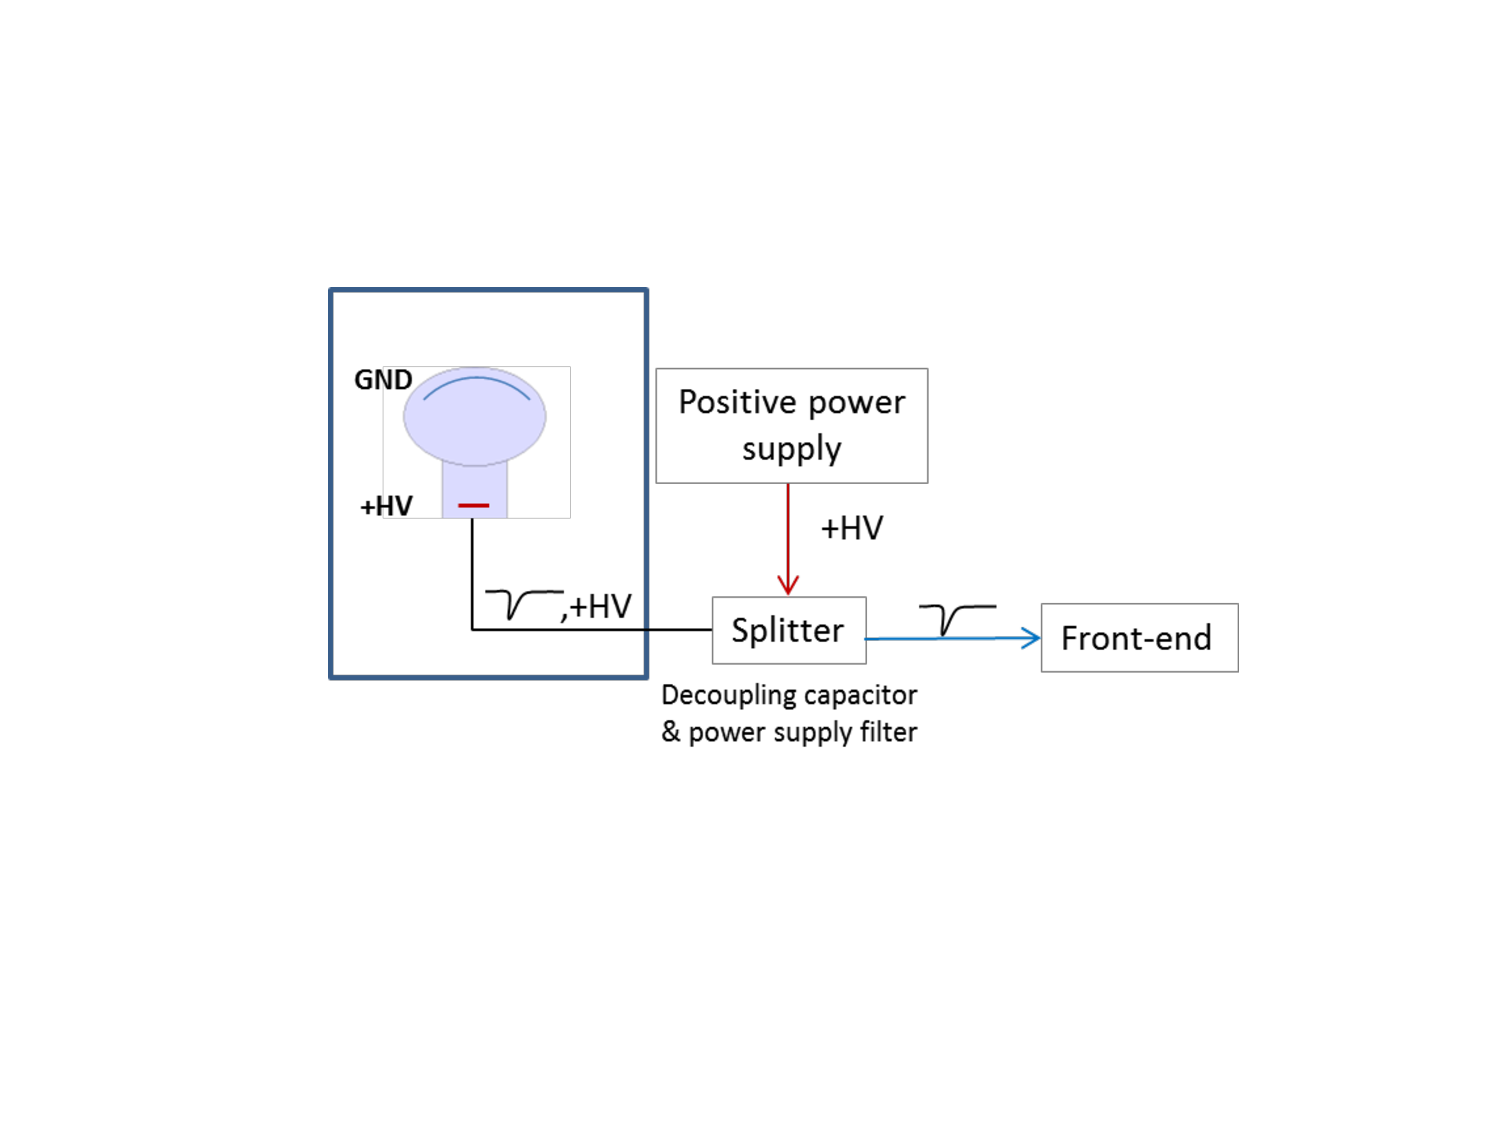
\includegraphics[width=0.6\textwidth]{dppd_4_1}
\end{dunefigure}

The \dword{pmt} base circuit uses only resistors and capacitors. The components are carefully selected and tested to minimize variations in their characteristics with temperature. The polarization current of the voltage divider (total circuit resistance) is chosen to fit the \dword{pmt} light linearity range (up to \SI{100}{PEs} per \SI{6}{\ns}, see Table~\ref{tab:specs:DP-PDS}) and maximum power requirements (\SI{<0.2}{W/\dword{pmt}}). The dynodes' voltage ratio will follow manufacturer recommendations for increasing linearity range on the space-charge effect area (tapered divider). In addition, capacitors are added to the last stages  to increase the \dword{pmt} linearity in pulsed mode.

The \dword{pmt} base connects to the \fdth with the RG-303/U cable, selected for its low attenuation and its proven reliability in cryogenic environments. The short cable is directly soldered to the \dword{pmt} base on one end and, on the other end, attaches to the long \dword{hv} cable with an SHV connector. The long cable connects to the feedthrough flange.


%%%%%%%%%%%%%%%%%%%%%%%%%%%%%%%%%
\subsection{High Voltage and Signal Splitters}
\label{sec:fddp-pd-4.2}

\Dword{hv} and signal splitters 
separate the fast \dword{pmt} response signal from the positive \dword{hv} with capacitive decoupling. 
A low-pass filter between the \dword{hv} supply and the \dword{pmt} reduces the noise.

It is possible for radiated \dword{emi} picked up by the cables, and for conducted noise from the \dword{hv} power supply, to be synchronous across many \dword{pmt} channels (i.e., coherent noise). This noise could add up to produce false detector triggers. Because the \dword{pmt} signal can be as low as a few \si{mV},
control of the \dword{emi} over the circuit is very important. The splitter \dword{hv} input filter should reduce the \dword{emi} induced and conducted by the power supply cables. Enclosing each splitter channel in its own metallic grounded box reduces the \dword{emi} directly received in the splitter circuit and 
the cross-talk between different splitter channels.

Figure \ref{fig:dppd_4_2} shows a generic splitter circuit where R1 and C1 form the \dword{hv} input low-pass filter (with a cut-off frequency below \SI{60}{Hz}). The resistor R7 and the  \dword{led} are for safety only, warning when \dword{hv} is applied to the splitter. The C4 capacitor splits the signal coming from the \dword{pmt} from the \dword{hv}, and R2 prevents the \dword{pmt} signal from going to ground through the C1 capacitor. R4 and R5 are \SI{0}{\ohm} optional resistors that allow some flexibility in the grounding configuration. Finally, R3 ensures the discharging of C4 if the splitter is not connected to the \SI{50}{\ohm} input at the \dword{daq} system. The RC time constant of the capacitor C4 and the load (\SI{50}{\ohm}) must be as large as possible to minimize baseline oscillations due to the charge-discharge of the capacitor. Values of C4 between \SI{150}{nF} and \SI{300}{nF} have already been tested. Figure \ref{fig:dppd_4_3} shows the \dword{hv}/signal splitter box of \dword{pddp}.

\begin{dunefigure}[Generic splitter circuit diagram]{fig:dppd_4_2}
{Generic splitter circuit diagram.}
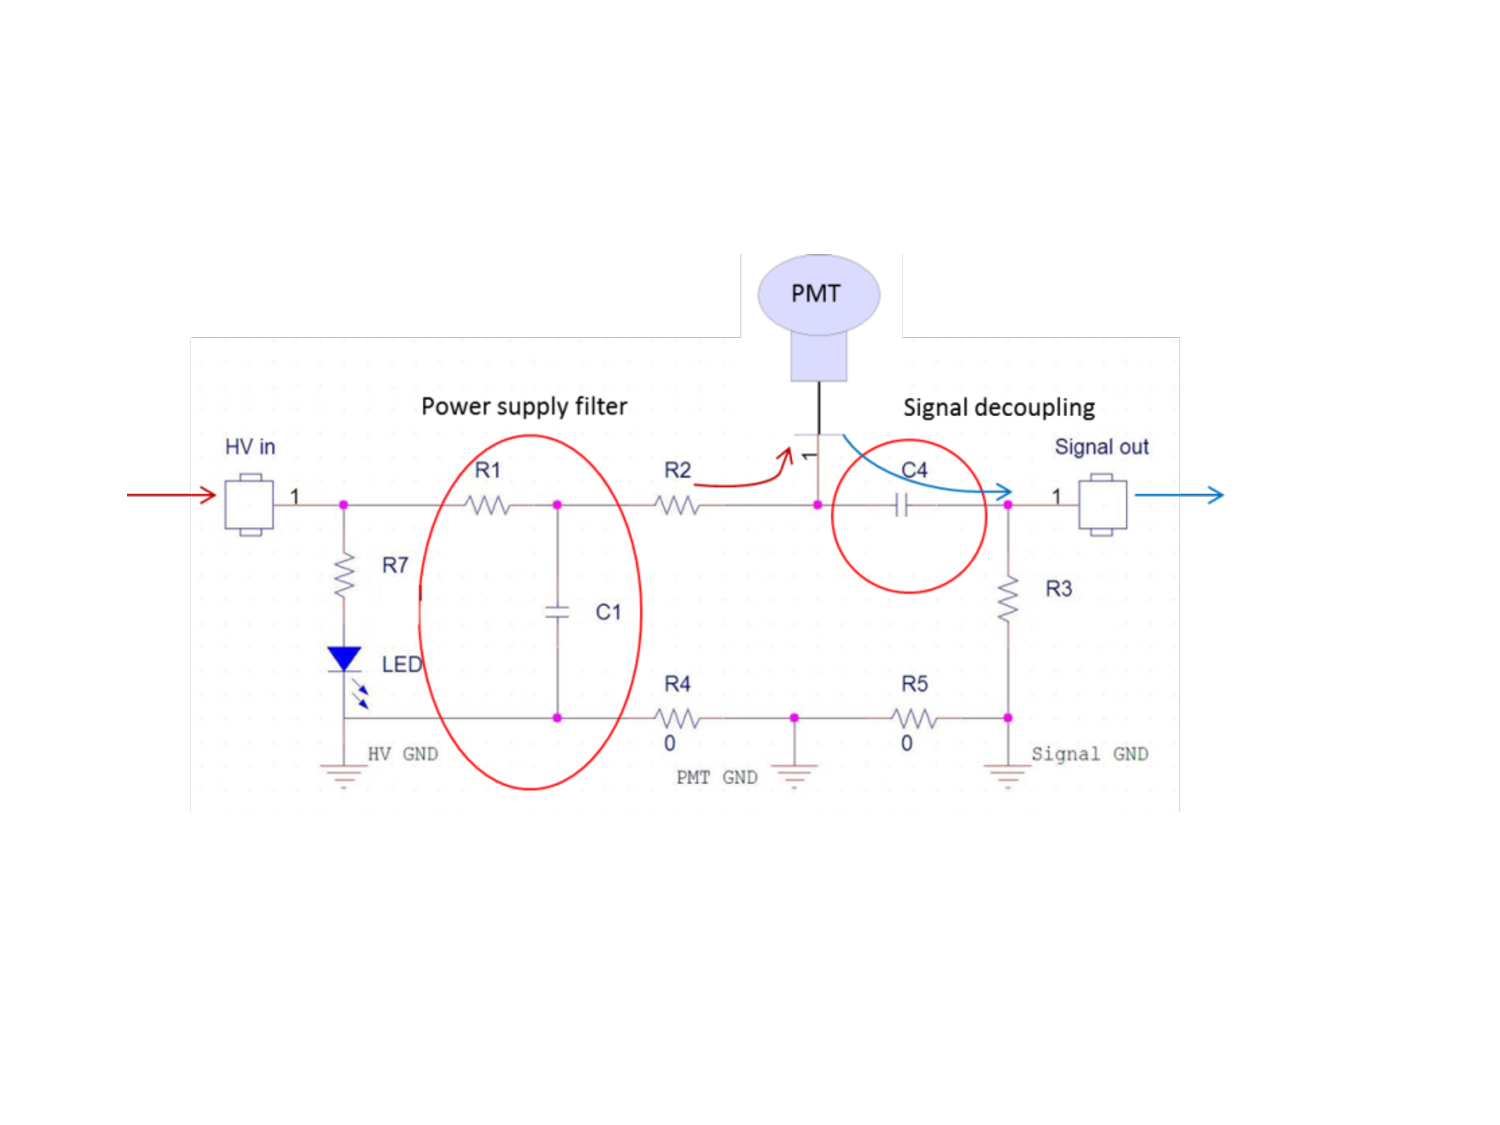
\includegraphics[width=0.85\textwidth]{dppd_4_2}
\end{dunefigure}

\begin{dunefigure}[Picture of the splitter box for \dshort{pddp}]{fig:dppd_4_3}
{Picture of the splitter box for \dword{pddp}.}
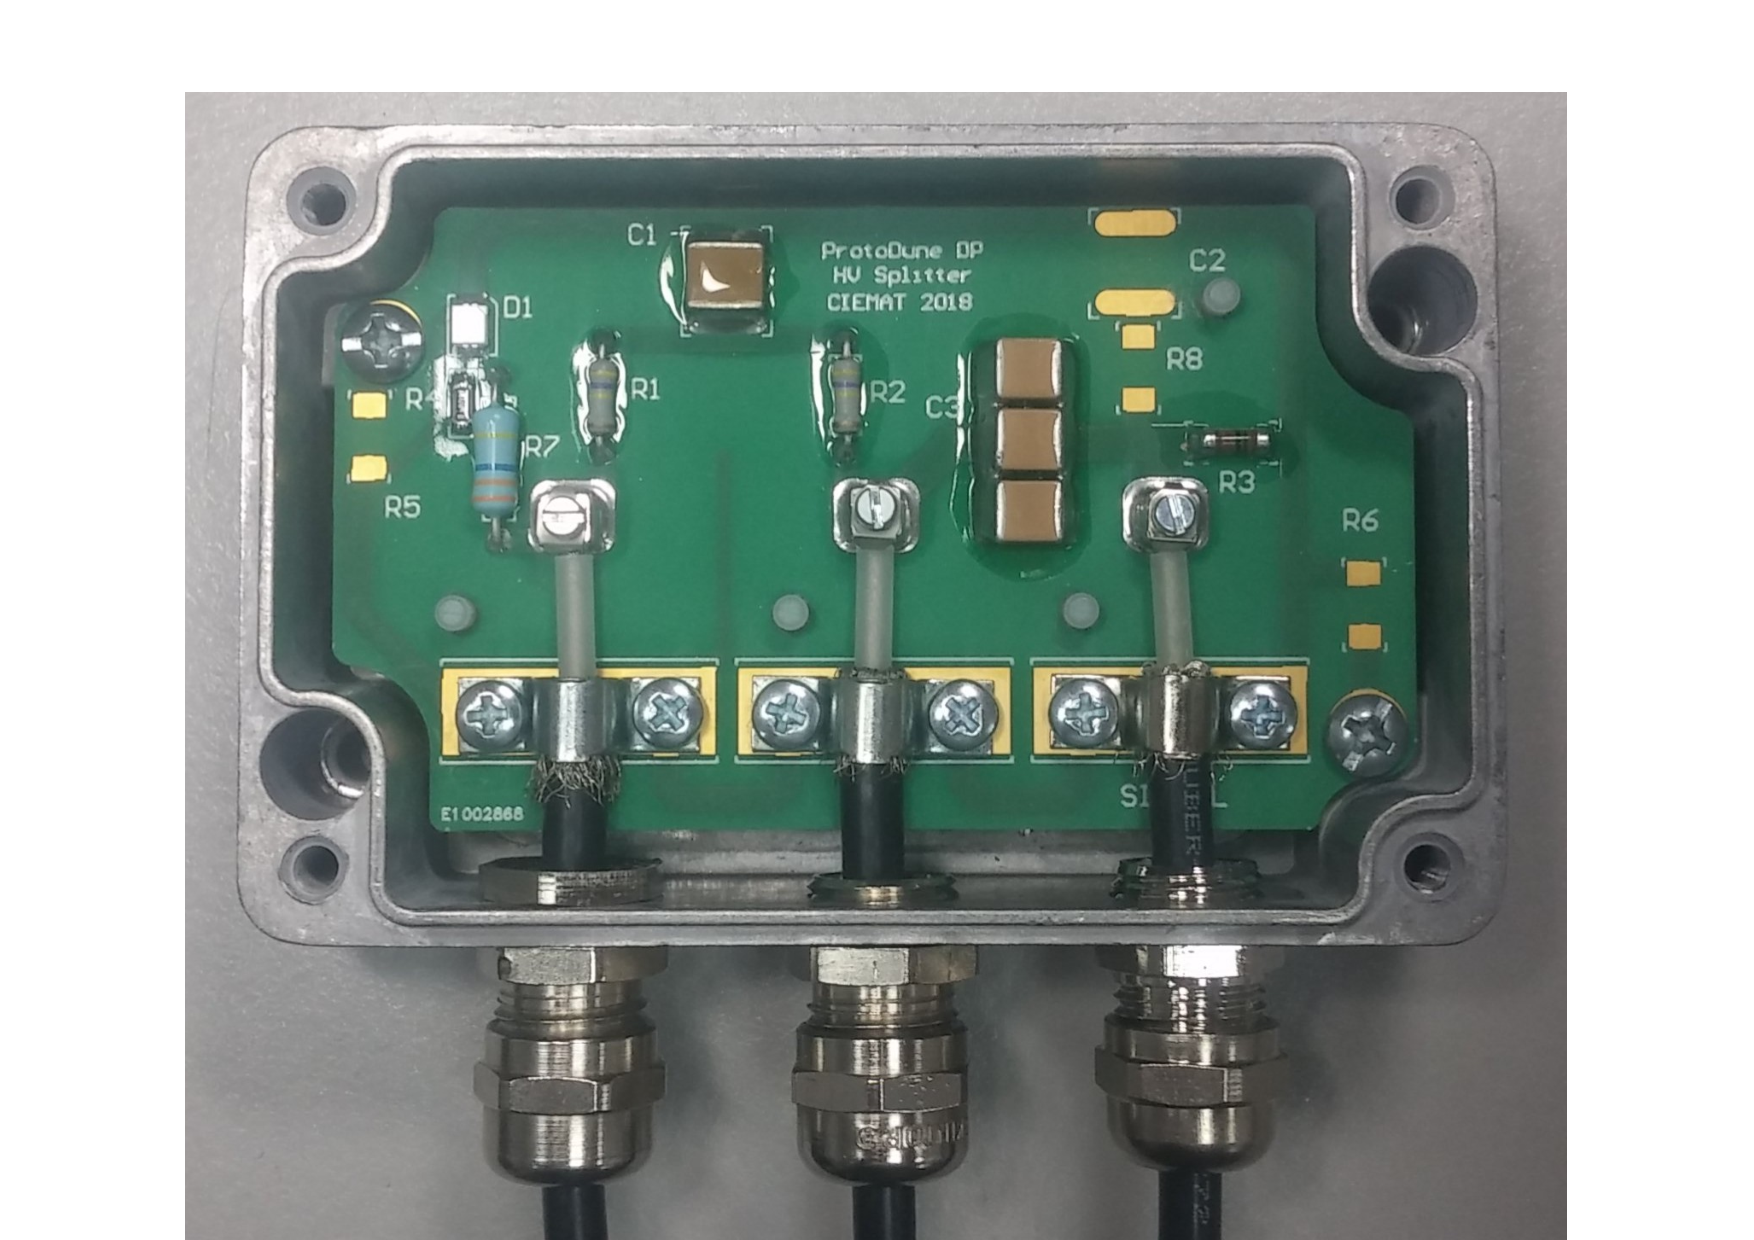
\includegraphics[width=0.5\textwidth]{dppd_4_n3}
\end{dunefigure}

For the connections between the \dword{hv} power supply and the splitters and between the splitters and the cryostat \fdth{}s, HTC 50-3-2 cables have been chosen as baseline. The HTC 50-3-2 has a similar attenuation as the RG-303/U (used inside the cryostat), but costs \numrange{8}{10} times less. Both cables are attached on one end directly to the \dword{hv} splitter and have an SHV connector on the other end. An RG-58 cable terminated on the connector required by the light readout card provides the connection between the splitter and the card. The \dword{pmt} readout card is described in Chapter~\ref{ch:dp-tpcelec}.


%%%%%%%%%%%%%%%%%%%%%%%%%%%%%%%%%
\subsection{Signal Readout}
\label{sec:fddp-pd-4.3}

To meet the physics requirements, the following is the information that must be extracted from the \dword{pmt} signals:

\begin{itemize}
\item S1 fast component shape, charge, and timing;
\item S1 slow component shape and charge;
\item S2 shape, charge, and timing (distance from S1 and duration);
\item \dword{spe} charge spectrum for gain calculation during \dword{pmt} calibration; and
\item trigger signal generation by the coincidence of several \dword{pmt} signals.
\end{itemize}


The requirements to both unambiguously reconstruct single-\phel short pulses and to avoid saturation of S1 light signals of hundreds of \phel{}s, integrated charge distributed over hundreds of nanoseconds determines the readout electronics parameters, in particular \dword{pmt} gain readout sampling time. The \dword{pmt} gains will be set to \num{1e7} and the sampling time to \SI{15.4}{ns}, as justified in the following. In general, the \dword{pmt} signal dynamic range goes from the \si{mV} level to several volts (over \SI{50}{\ohm} load). The lower limit of the \dword{pmt} dynamic range is given by the lowest level of the \dword{spe} signal that meets the \dword{s/n} ratio specification. Thus, the \dword{pmt} gain should be set at least at the value that makes the \dword{spe} level meet this condition. Figure~\ref{fig:dppd_4_3_ab} shows the \dword{spe} waveforms (left) and amplitudes from the WA105 at different voltages (right).

\begin{dunefigure}[\dshort{spe} waveforms and amplitudes from the WA105 at different voltages]{fig:dppd_4_3_ab}{\dword{spe} waveforms (left) and amplitudes from the WA105 at different voltages (right).}
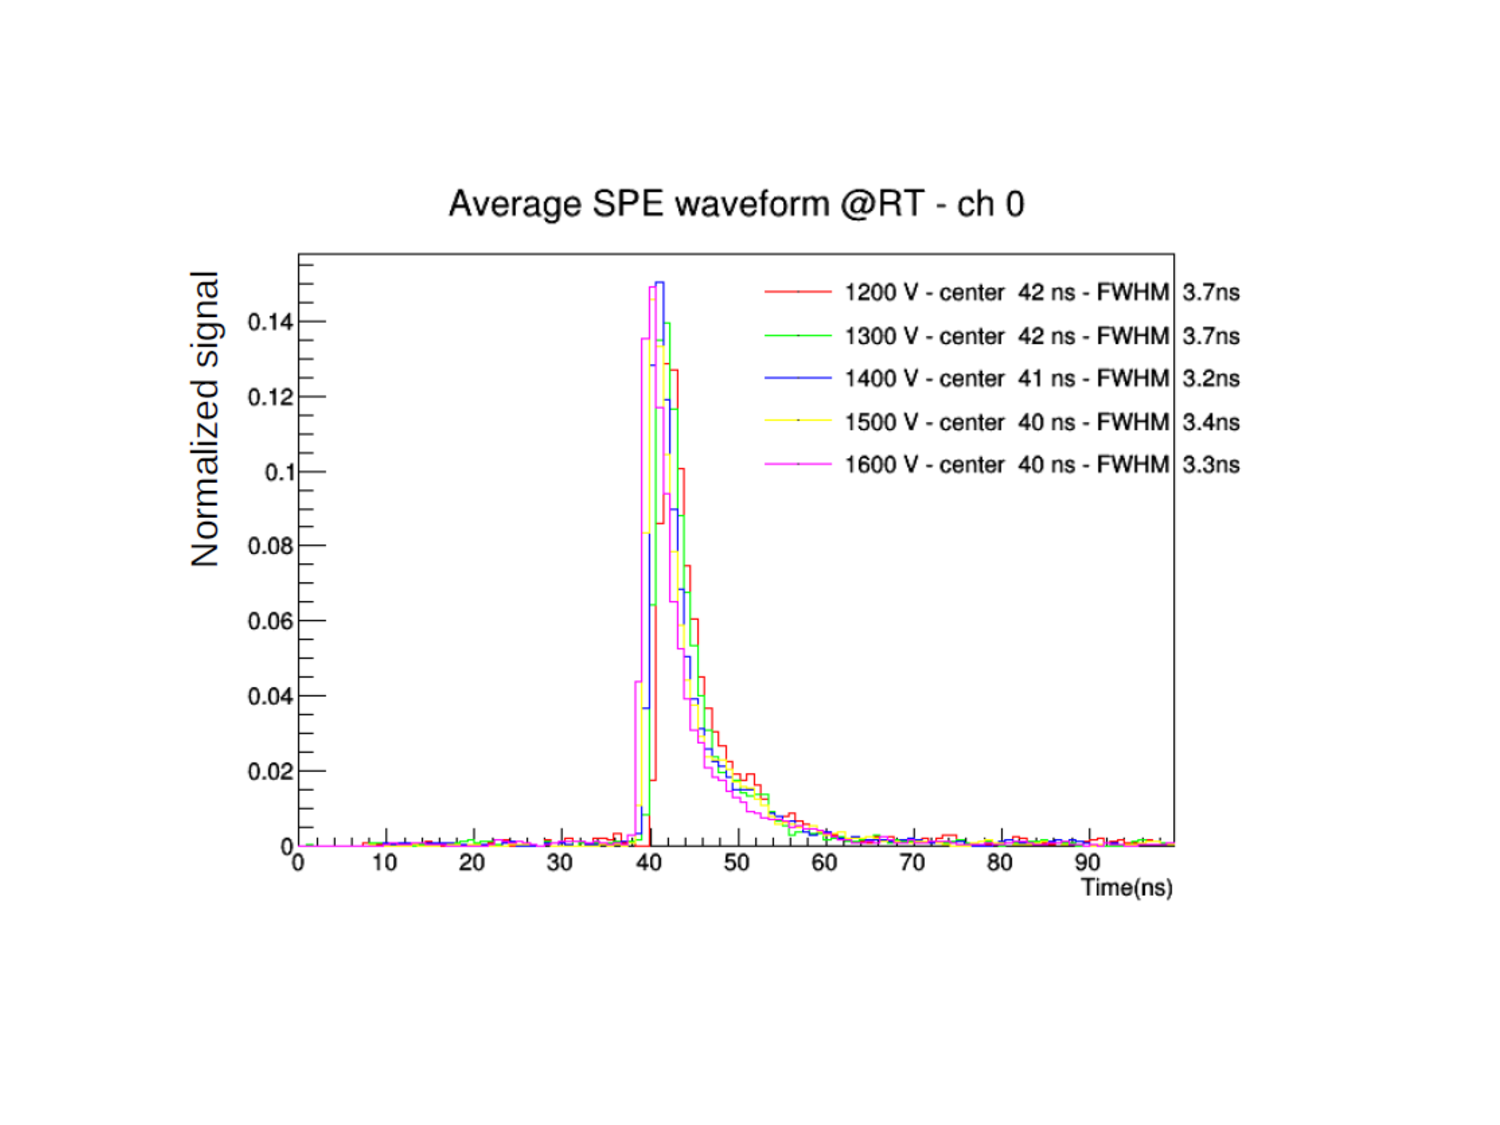
\includegraphics[width=0.47\textwidth]{dppd_4_3_a}
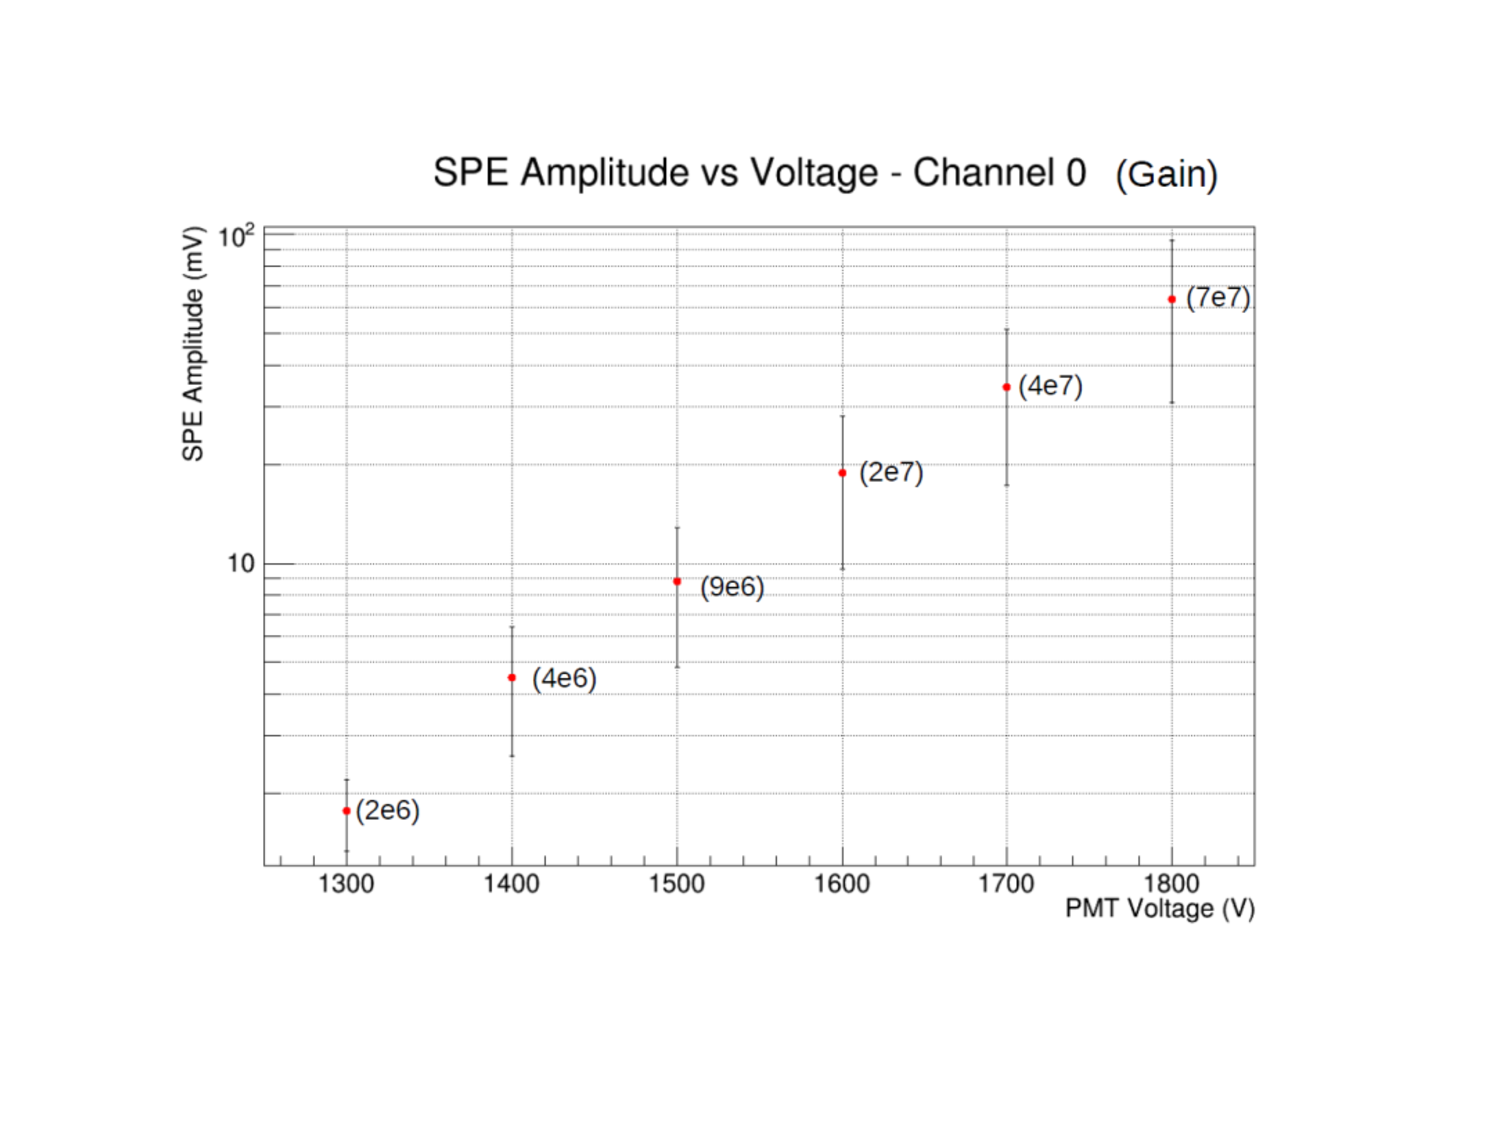
\includegraphics[width=0.47\textwidth]{dppd_4_3_b}
\end{dunefigure}

Because the %long 
cables from the \dwords{pmt} to the \dword{fe} electronics are very long, the cable noise could be high. If a noise level around \SI{1}{mV} is considered,  the \dword{pmt} gain must be set to \num{e7} or higher to have the required \dword{s/n} ratio of 5, see Table~\ref{tab:specs:DP-PDS}. The average \dword{spe} pulse width is approximately \SI{3.5}{ns} \dword{fwhm}. If an accurate signal reconstruction is required, the sampling period should be of the level of the \si{\ns}. Since only charge information and approximate timing information (at the level of $<\,\SI{100}{ns}$ RMS hit time resolution, see Table~\ref{tab:specs:DP-PDS}) is necessary, the sampling period can be higher, but the signal must be low-pass filtered before sampling. This filtering affects the signal level making the discrimination of signal from noise more difficult, requiring an increase of the \dword{pmt} gain to meet the \dword{s/n} specification. 


The upper limit of the required dynamic range is given by the \dword{pmt} signal amplitude for the maximum number of \dwords{pe} expected per sampling time unit. As shown in Figure~\ref{fig:dppd_saturation} for simulated \SI{3}{GeV} beam neutrino interactions, the maximum number expected in this case is about \SI{60}{PEs} for a fast sampling of \SI{4}{ns} and about \SI{500}{PEs} for sampling times comparable to S1 signal durations (about \SI{1}{\micro\second}) or slower. Hence, while single-\phel signals can  still be detected with slow sampling times by adjusting the \dword{pmt} gain accordingly, the dynamic range requirement becomes more stringent. 

The time sampling of the \dword{pds} waveforms will be \SI{15.4}{ns}, as provided by the \SI{65}{MHz} \dword{adc} in the \dword{lro} electronics card (see Section~\ref{ch:dp-tpcelec}). Similar readout electronics parameters as the baseline ones described here are being validated in \dword{pddp}, and are found to meet our specifications. In particular, Hamamatsu R5912-MOD20 \dwords{pmt} operated at a gain of \num{1e7} and whose signals are digitized at a \SI{16}{ns} sampling period yield a single-\dword{pe} \dword{s/n} ratio in excess of the required \dword{s/n}=5 value.


The light signal must be synchronized with the \dword{daq}. All \dword{daq} electronics use the \dword{wr} protocol for synchronization. A dedicated \dword{wr} \dword{utca}~\cite{utca} slave node is on the light readout \dword{fe} electronics as sync receiver, distributing clocks to different \dword{fe} cards.


\section{Calibration System}
\label{sec:dp-pds-calibration}

A photon calibration system is required in the \dword{dpmod} to calibrate the \dwords{pmt} installed in the \dword{lar} volume. The goal is to determine the \dword{pmt} gain and monitor the stability of the \dword{pmt} response. One of the main goals of the \dword{pds} is to provide a trigger for non-beam physics. The trigger is based on the amplitude of \dword{pmt} signals. The amplitudes of the \dword{pmt} signals are summed for groups of certain \dwords{pmt} and/or for all \dwords{pmt} and then, these input signals are discriminated according to the trigger logic. An equalized \dword{pmt} response allows using the same threshold definition for all \dword{pmt} groups, simplifying the determination of trigger efficiency. In addition to measuring the \dword{pmt} gain, the calibration system is also designed to monitor the stability of the \dword{pmt} response. % and its quantum efficiency.
Therefore, the calibration system must be able to illuminate all \dwords{pmt} at \dword{spe} level and at larger light intensities to ensure that the gain calibration and linearity can be determined from the data. Given the necessary \dword{pmt} characterization at cryogenic temperature before installation~\cite{Belver:2018erf}, and based on past experience with \dword{wa105} %detector 
operations~\cite{Aimard:2018yxp}, we conclude that a light calibration system is needed during experiment data taking.

%%%%%%%%%%%%%%%%%%%%%%%%%%%%%%%%%%%%%%%%%%%%%%%%%%%%%%%%%%%%%%%%%%%%

\subsection{Calibration System Design}

An \dword{led}-driven fiber calibration system~\cite{Cuesta:2017nrs,Conrad:2015xta,Caccianiga:2003fm,ADAMSON2002325,Belver:2019lqm} is designed such that a configurable amount of light reaches each \dword{pmt}. The calibration light is provided by a blue \dword{led} of \SI{465}{\nm} using a Kapustinsky~\cite{KAPUSTINSKY1985612} circuit as \dword{led} driver and transmitted by a fiber system ending with an optical fiber installed at each \dword{pmt} (see Figure~\ref{dppd-6-LCS}). Twenty groups of six \dwords{led} placed in a hexagonal geometry and a reference sensor check the performance of the \dword{led} in the center of each group. The direct light goes to the fiber, and the stray light to the \dword{sipm} used as reference sensor. Each \dword{led} is connected to an external fiber going to one feedthrough. Then, fibers are connected inside the cryostat, and each fiber is attached to a 1-to-7 fiber bundle, so that one fiber is finally installed pointing at each \dword{pmt}. The \dwords{pmt} are oriented with the first dynode perpendicular to the Earth magnetic field and the fiber parallel to the first dynode to have a similar gain to the one obtained with diffuse light. The components placed outside the cryostat at room temperature form the ``external system,'' and the ones installed inside it at cryogenic temperature form the ``inner system.'' 

\begin{dunefigure}[\dshort{pds} light calibration system]{dppd-6-LCS}
{Sketch of the \dword{dune} \dword{fd} \dword{pds} light calibration system. The external system at room temperature is shown in blue and the inner system at cryogenic temperature in black.}
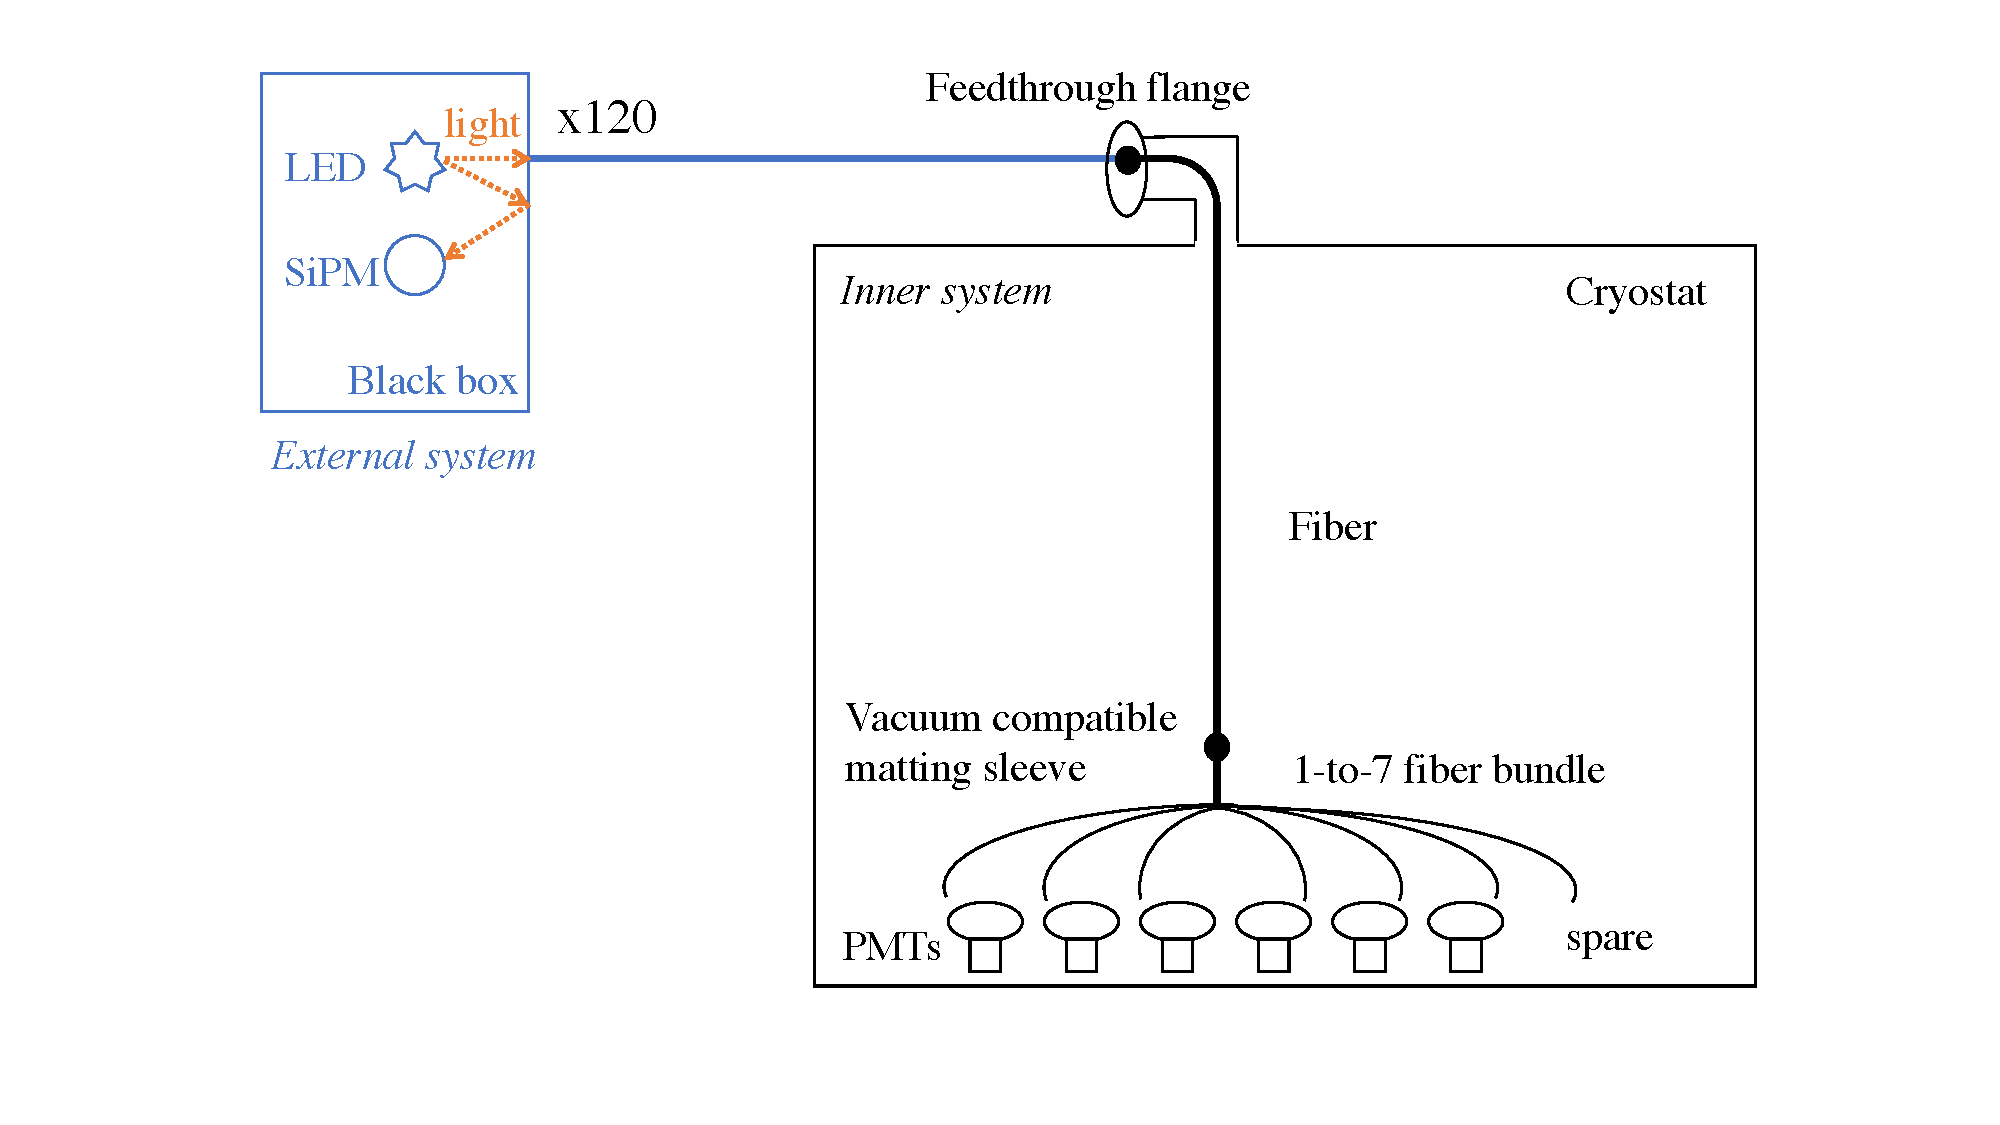
\includegraphics[width=0.7\textwidth]{dppd_LCSdiagram_DUNE}
\end{dunefigure}


%%External system
The design of the external components is driven by the need for a cost-effective system. An additional requirement is that a reference light sensor monitor the amount of injected light. The light is injected in the form of several \si{\ns} long pulses provided by a Kapustinsky circuit. The set up consists of a commercial black box in which a light guide structure is mounted. There are \num{20} structures, and each has six arms and a central part, as shown in Figure~\ref{fig_source}. On each of the six arms, an electronics board containing a Kapustinsky circuit is mounted. The \dword{led}, NSPB300B from Nichia Corp.\footnote{www.nichia.com}, with a peak wavelength of \SI{465}{nm} is placed  on the \dword{pcb} in front of an optical SMA to SMA \fixme{what's SMA?} feedthrough. On the other side of each feedthrough, an optical fiber, FG105LCA-CUSTOM-MUC from Thorlabs\footnote{www.thorlabs.com}, is connected. The fiber transports the light to one of the \num{120} feedthroughs in the instrumentation flange on top of the cryostat. While a large fraction of the \dword{led} light is emitted forward, a small fraction, the stray light, is emitted under a large angle and reaches by reflection to the central region of the light guide structure where it is detected by a \dword{sipm}, MicroFJ-30035-TSV-TA from SensL\footnote{www.sensl.com}.


\begin{dunefigure}[Light guide structure during  development and light path]{fig_source}
{(Left) Picture of the light guide structure during the development phase. The six arms are visible, and on one of them a prototype \dword{led} driver is mounted. (Right) Schematics of the light way from the \dword{led} to the reference sensor.}
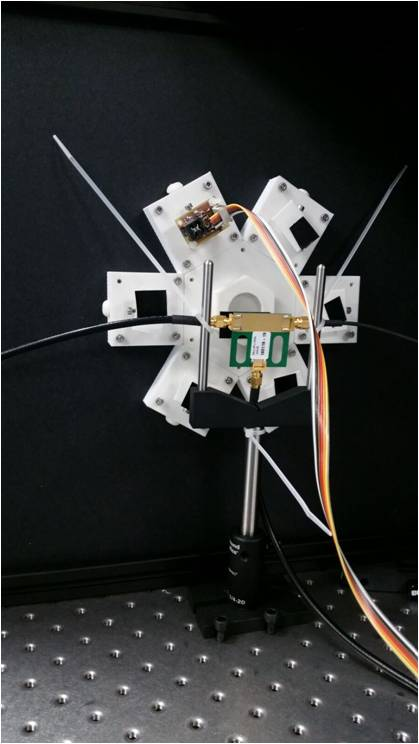
\includegraphics[width=0.25\textwidth]{dppd_LightGuide.jpg}
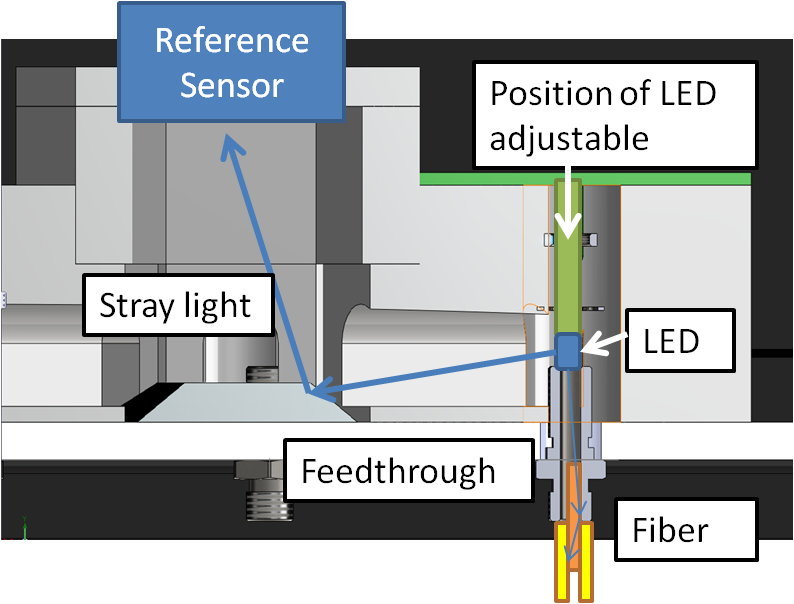
\includegraphics[width=0.6\textwidth]{dppd_Stray.png}
\end{dunefigure}




%############################################

%%Inner system
The inner system is designed to minimize light losses at cryogenic temperatures. The external fibers are connected to 120 female optical feedthroughs from Allectra\footnote{www.allectra.com} installed at \num{20} flanges. Inside the cryostat, a single long fiber, FT800UMT from Thorlabs, goes down from each optical feedthrough routed along the walls of the cryostat to the bottom of the cryostat where a \num{1}-to-\num{7} fiber bundle, comprising FT200UMT fibers from Thorlabs, is connected to each long fiber. A total of \num{720} of these fibers are guided to the \dwords{pmt} at the bottom of the detector. The end of the fiber is fixed at the \dword{pmt} support structure pointing the photocathode. The fibers and bundles are \num{0.39}\,NA TECS$^\text{TM}$ hard-clad, multimode, step-index fibers with high OH (hydroxyl) content to increase the light transmission at low wavelengths. To optimize the light transmission of the fiber-bundle connection, the inner fibers have a diameter of \SI{800}{\um}, big enough to distribute uniformly the light at the bundle entrance, total diameter \SI{700}{\um}. \fixme{check numbers and units} From the mechanical point of view, the described approach of bundles attached to fibers is safer than connecting  the bundles directly to the feedthroughs. To have good homogeneity of the light at the fiber-bundle connections, SMA connectors are chosen. Vacuum-compatible SMA to SMA mating sleeves are required in order to avoid \dword{lar} freezing inside the connector, which would reduce light transmission.

Three different measurements will be performed during the detector operation:
\begin{itemize}
    \item Gain stability: \dword{spe} spectrum at the \dword{pmt} operating \dword{hv} will be measured to obtain the gain. This measurement will be taken every time the \dwords{pmt} are biased up, and regularly, every day at the beginning, and every few days when stable operating conditions are reached. Considering that high \dword{led} repetition rates can be used \cite{Belver:2019lqm}, sufficient \dword{spe} statistics can be acquired in less than one minute. 
    \item Gain vs. \dword{hv}: \dword{spe} spectrum at different \dword{pmt} voltages (\SI{1300}{\V} - \SI{1900}{V} in \SI{200}{V} steps) to obtain the gain calibration curve. This measurement will be taken every time the operating conditions change. It can be performed occasionally when stable operating conditions are reached, also considering that a full gain versus high voltage scan can be taken in only a few minutes .  
    \item Light response: The \dword{led} voltage can be increased to study the \dword{pmt} performance for different light intensities from the \dword{spe} to several tens of photo-electrons.
\end{itemize}

Alternatives to the calibration system baseline design described here are also being considered. See Appendix~\ref{sec:dp-pds-appendix-calibration}. 



\section{Photon Detector Simulation}
\label{sec:dp-pds-simulation}

A detailed simulation of the \dshort{pds} response is essential both to compare with data from \dshort{pds} prototypes (see Section~\ref{sec:dp-pds-prototypes}) and to validate the \dword{fd} baseline design for its projected performance (see Section~\ref{sec:dp-pds-performance}).

%%%%%%%%%%%%%%%%%%%%%%%%%%%%%%%%%%%%%%%%%%%%%%%%%%%%%%%%%%%%%%%%%%%

\subsection{Simulation Framework And Assumptions}
\label{subsec:dp-pds-simulation_assumptions}

The simulation of the \dword{pds} response is integrated in \dword{larsoft}, the liquid argon software toolkit used by the \dune Collaboration for simulation and reconstruction. The simulation is divided in three steps: light generation, light propagation, and light detection.

For a \dword{mip}, an energy of about \SI{2}{\MeV/\cm} is deposited in \dword{lar}. Through decays of excited argon states and ion recombination, about \num{40000} scintillation photons are emitted per \si{\MeV} deposited at null drift field. At the nominal drift field of \SI{500}{\V/\cm}, this amount reduces down to about \num{24000} photons per \si{\MeV} as the recombination process weakens. This signal, known as S1 (see Section~\ref{sec:dp-pds-overview}), is common to the single and dual phase technologies.

In the gas layer of the dual phase design, the electrons are amplified through Townsend avalanche in the \dword{lem} holes and lead to an electroluminescence signal called S2 (see Section~\ref{sec:dp-pds-overview}). The electroluminescence gain, $G_{EL}$, i.e., the number of photons produced per electron crossing the liquid-gas interface, depends on the voltages applied to the \dword{lem}. In our simulations, we typically assume a gain of \SI{300}{photons per extracted electron}. The S1 and S2 signals have similar characteristics for wavelength and time constants. 

Because of different mechanisms during photon propagation (Rayleigh scattering, absorption by impurities in the \lar or by elements constituting the detector), only \num{1e-3} fraction of the photons produced in the \lar active volume reaches the \dword{pmt} photo-cathodes. The direct simulation of the large number of photons generated for each track crossing the active volume would require a considerable amount of CPU power and time. Profiting from the fact that the photon emission is isotropic and the detector is uniform and symmetric, it was decided to generate the photon propagation in the detector in a dedicated Geant4 simulation only once and then to store the results in a photon library.

The active volume is divided into voxels, and a large number of photons are isotropically and uniformly generated in every voxel. The number of photons collected by each \dword{pmt} and the propagation time are stored and later parametrized. For long voxel-\dword{pmt} distances (typically larger than \SI{1}{\m}), a Landau function is well suited to reproduce the time distribution. The detection probability, called visibility, the landau parameters (most probable value, $\sigma$) and the minimal time needed by the photon to reach the \dword{pmt} are stored in a photon library for all voxel-\dword{pmt} combinations. When a track is generated in the standard \dual \dword{larsoft} simulation toolkit, for each step of the track, the light map is looked up to assign the number of photons to be collected at each \dword{pmt} and the arrival time distribution due to the propagation. 

To generate photon libraries, a comprehensive modelling of the geometry for the \dword{wa105}, \dword{pddp}, and \dword{dp} \dword{fd} detectors are implemented in \dword{gdml} files. The \dword{gdml} files include the main elements relevant for light propagation, such as the cathode, the \dword{fc}, the \dwords{lem}, and the ground grid. Most detector elements are assumed to be fully absorptive. Thus, when photons reach any of these surfaces, they are removed from the simulation. One exception is \dword{wls} reflector foil surfaces, which are assumed to have \SI{100}{\%} \dshort{wls} efficiency for \SI{127}{\nm} \dshort{lar} light and 93\% reflectivity for \SI{430}{\nm} light re-emitted by the wavelength shifter material. To quantify the effect of the \dshort{wls} reflector foils for the \dword{dp} \dword{fd} module, three geometries have been tested: no foils, foils entirely covering all four \dword{fc} vertical walls (full foils, in the following), and foils covering only the upper half of the \dword{fc} (half foils, in the following). For the \dword{pds} prototypes, no foil geometries have been simulated.

As far as \dword{lar} optical properties are concerned, the simulations assume a \SI{61}{\cm} Rayleigh scattering length for \SI{127}{\nm} light, no Rayleigh scattering for visible light, and a \SI{20}{\m} absorption length for all wavelengths. The response of the \dword{pmt} is simulated assuming an effective quantum efficiency of \num{0.12} for \SI{127}{\nm} light. This value includes the \dword{tpb} response of the coated photo-cathode \cite{Bonesini:2018ubd}. For visible light emitted by \dword{wls} foils, the \dword{pmt} quantum efficiency is taken to be \num{0.20}. A dark count rate of \SI{1.7}{\kilo\hertz} at cryogenic temperature is assumed, as obtained during \dword{pddp} \dword{pmt} calibration \cite{Belver:2018erf}. A linear response of the \dword{pmt} is assumed, multiplying the number of photons reaching the photo-cathode with the single photo-electron response measured in the laboratory for a gain of \num{1e7}. In this case, the single-PE response has a time width of \SI{6}{\nano\s}, and an amplitude of \SI{15}{mV}. The digitization of the waveform is simulated considering a sampling rate of \SI{250}{MHz}\footnote{This is the sampling frequency used in the \dshort{wa105} readout, but slower frequencies of \SI{65}{MHz} or \SI{2.5}{MHz} are being considered for the \dword{dp} \dword{pds}.}, a resolution of \SI{0.5}{mV/ADC}, and an electronics noise of \SI{0.8}{ADC counts \dword{rms}} as measured in \dshort{wa105}, see Section~\ref{sec:dp-pds-prototypes}. Therefore, based on \dshort{wa105} measurements, the \dword{spe} to baseline noise \dword{rms} ratio assumed in the simulations exceeds \num{30}.

%%%%%%%%%%%%%%%%%%%%%%%%%%%%%%%%%%%%%%%%%%%%%%%%%%%%%%%%%%%%%%%%%%%

\subsection{Expected Light Yields}
\label{subsec:dp-pds-simulation_yields}

Table~\ref{tab:dp-pds-light-yields} gives the detected light yields expected in the \dune \dword{fd} geometry, for the three different \dword{wls} reflector foil geometries mentioned above. The yield is computed by averaging over all \lar voxels contained in the \dword{tpc} active volume. A voxel size of \SI{1}{\m^3} is considered in \dword{dp} \dshort{fd} simulations. The average yield is \num{5.4}, \num{8.0} and \SI{12.2}{PEs/MeV} for the no foils, half foils and full foils geometries, respectively. The higher yield for the foil geometries is partly due to the higher number of photons reaching the \dword{pmt} photo-cathodes, and partly due to the higher \dword{pmt} quantum efficiency for visible light. As shown in Table~\ref{tab:dp-pds-light-yields}, a 11.3\% (33.8\%) fraction of photons reaching the \dwords{pmt} is \dword{wls} visible light, in the half foils (full foils) geometry.

\begin{dunetable}
[Average light yields in the DUNE FD geometry.]
{crrr}
{tab:dp-pds-light-yields}
{Average light yields in the \dune \dword{fd} geometry for different \dword{wls} reflector foil configurations. The total incident light yields and the fractions of incident \dword{wls} light at the \dword{pmt} photo-cathodes, as well as the total detected light yields, are given.}
Configuration & Incident light yield & Fraction of incident & Detected light yield \\
\rowcolor{dunesky} 
 & (photons/\si{MeV}) & \dword{wls} light (\%) & (PEs/\si{MeV}) \\ \toprowrule
%\hline
No Foils   &  45 &  0.0 &  5.4 \\ \colhline
Half Foils &  62 & 11.3 &  8.0 \\ \colhline
Full Foils &  83 & 33.8 & 12.2 \\ 
%\hline
\end{dunetable}

\begin{dunefigure}[Expected 1D light yields in the full DP detector module]{fig:dppd_fd_light_yield_comparisons}
{Expected light yield in the full \dword{dp} \dshort{fd} cryostat. The yield units are number of photo-electrons per \si{\MeV} of deposited energy. The 1D yields are shown as a function of the drift (transverse) direction in the left (right) panel, averaging over the other two spatial coordinates (not shown). The three histograms correspond to three different geometries: no \dword{wls} reflector foils, foils fully covering \dword{fc}, foils covering upper \dword{fc} half.}
\raisebox{0.1cm}{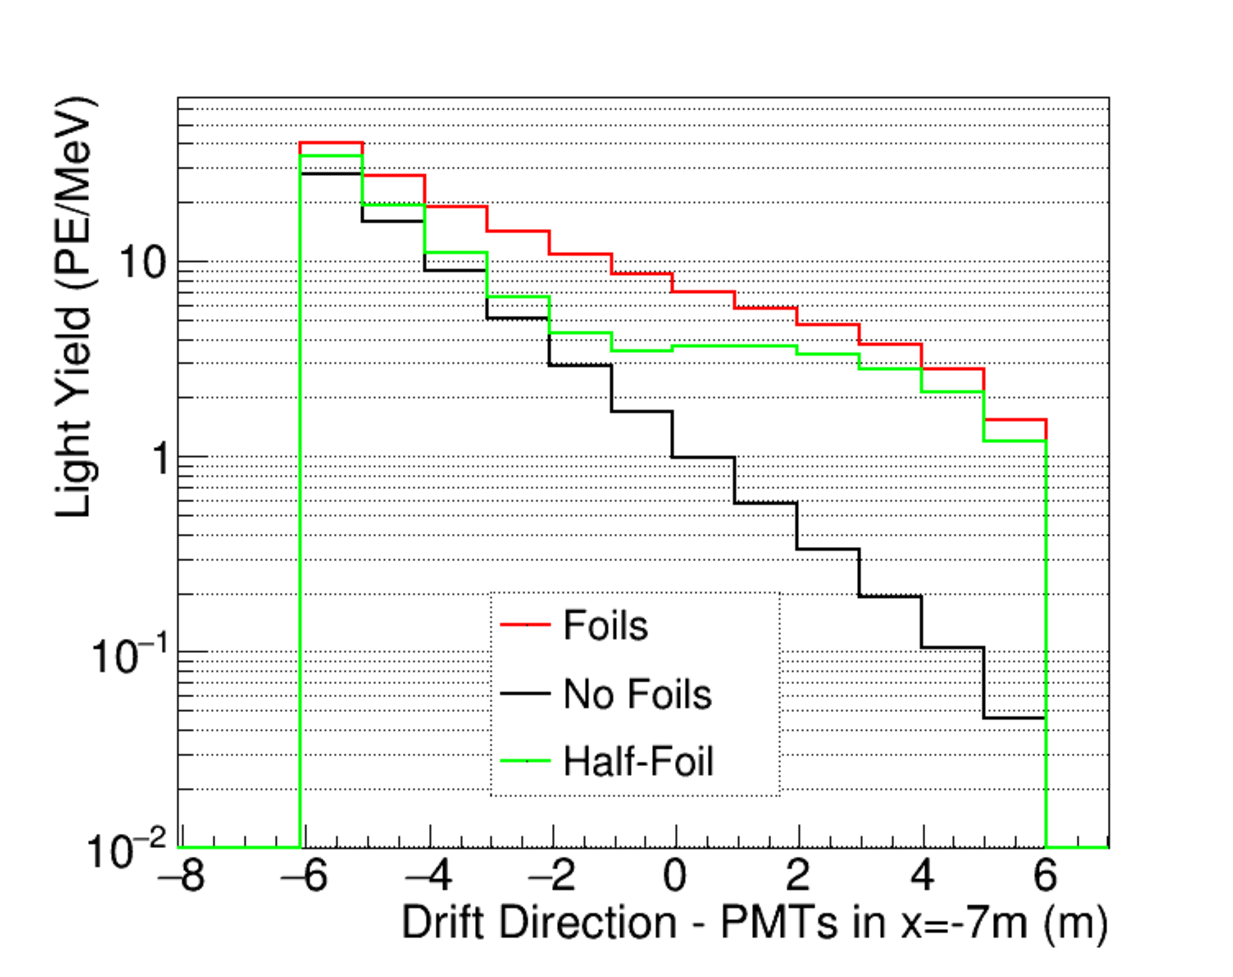
\includegraphics[width=0.49\textwidth]{graphics/dppd_PhotLibProjectionComparison_Drift.pdf}} \hfill
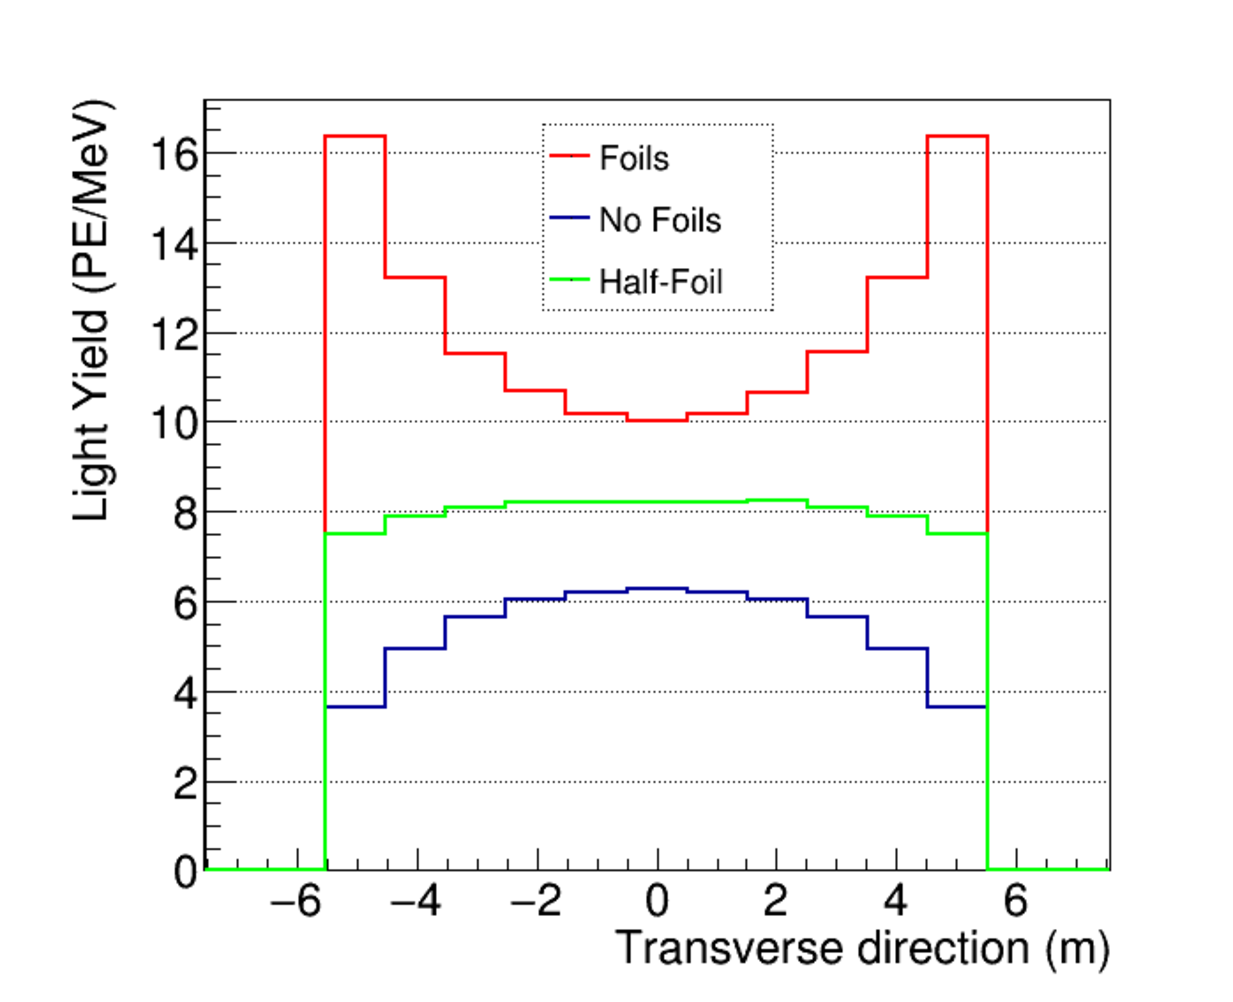
\includegraphics[width=0.49\textwidth]{graphics/dppd_PhotLibProjectionComparison_Trans.pdf}
\end{dunefigure}

We can also see the effect of the \dword{wls} reflector foils on the expected light yields in Figure~\ref{fig:dppd_fd_light_yield_comparisons}, where the yields are shown as a function of the drift coordinate (left panel) and transverse coordinate (right panel), and averaging over the two other spatial coordinates. The drift coordinate is the vertical one, while the transverse coordinate is the horizontal direction perpendicular to the neutrino beam direction. The left panel provides better appreciation of the main trend in the spatial response, namely the light yield reduction with increasing distance from the cathode. The \dword{wls} reflector foils are particularly useful in improving the yields at small drift distances, where the yields are lower. The foils reduce the very large non-uniformity in spatial response between cathode and anode by more than one order of magnitude. The full foils geometry provides better yields than half foils in the lower half of the detector. The difference between the two geometries is less significant at small drift distances. Being the most inefficient region of the \dword{pds}, the latter is the most important one to optimize through foils. In addition, the right panel shows that the half foils geometry is the one providing the best uniformity along the transverse direction. These plots justify why the half \dword{wls} foils geometry has been selected for the \dword{pds} baseline design.     

\begin{dunefigure}[Expected \twod light yield in the full DP detector module]{fig:dppd_fd_light_yield}
{Expected light yield in the full \dword{dp} \dshort{fd} cryostat, for the half \dword{wls} reflector foils geometry. The yield units are number of \phel{}s per \si{\MeV} of deposited energy. The \twod yield is shown as a function of the drift (vertical axis) and transverse (horizontal axis) directions, averaging over the third spatial coordinate (not shown). The red contours indicate the \dshort{tpc} active volume. The \dwords{pmt} are located at a drift coordinate of \SI{-7}{\m}.}
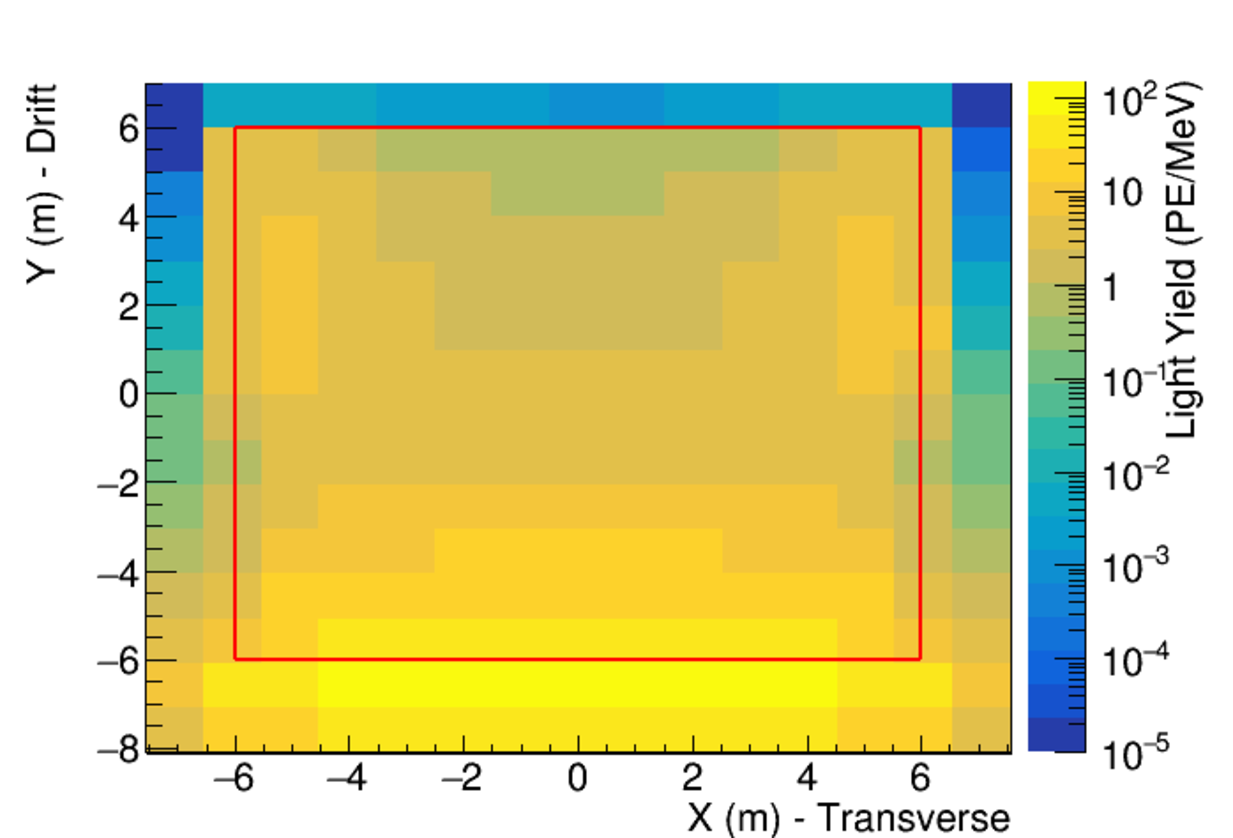
\includegraphics[width=0.65\textwidth]{graphics/dppd_PhotLibHalfFoil_longuerrange.pdf} 
\end{dunefigure}

Figure~\ref{fig:dppd_fd_light_yield} shows the detected light yield, for the half foils baseline geometry, as a function of drift and transverse directions simultaneously, and averaging over the beam direction. Near the cathode plane ($Y=$\SI{-6}{m} in this figure) the highest light yield is expected near the center of the active volume ($X=0$). The opposite is true near the anode plane ($Y=$\SI{+6}{m}).  


\section{Validation with Data from Photon Detector System Prototypes}
\label{sec:dp-pds-prototypes}

The \dword{lar} \dword{tpc} \dword{dp} proposed technology is the result of years of R\&D. From small-scale chambers to the \dword{dune} module, many prototypes have been constructed, each with some design modifications and optimizations. 
Relevant to the \dword{pds} itself, the \dword{wa105}, operated at CERN in 2017, the \dword{pddp}, to be commissioned in 2019 and the \dword{dune} far detector module similarities and differences will be described here.

\subsection{Design Comparison between Prototypes and Far Detector System}
%Similarities and Differences
The first tonne scale dual phase \dword{lar} \dword{tpc} demonstrator took cosmic data between June and November \num{2017} at CERN. 
Located \SI{1}{m} below the charge collection plane, underneath the cathode and the \dword{gg}, the photon detection system consisted of five \dwords{pmt} (Hamamatsu R5912-MOD20, described in more detail in Section~\ref{sec:dp-pds-photosensors}) evenly distributed along the 3$\times$1~m$^2$ area (one \dword{pmt} every \SI{50}{cm}). The demonstrator was an opportunity to test different \dword{pds} designs, particularly the \dword{tpb} coating and \dword{pmt} bases. Three \dwords{pmt} had the \dword{tpb} coating applied directly onto their windows using evaporation, but for the other two, the \dword{tpb} was deposited on a \SI{4}{\mm} thick transparent Plexiglass plate mounted on top of the \dwords{pmt}. 
While the latter solution has the advantage of being simpler and less risky to manipulate, it reduces acceptance and possibly efficiency because of the internal reflections between the \dword{tpb} and the Plexiglass surfaces. 
Pictures of the \dword{wa105} \dword{pds} are shown in Figure~\ref{fig:pd-pds-311-pmt-tpb}.

\begin{dunefigure}[\dshort{wa105} \dshort{pds} ]{fig:pd-pds-311-pmt-tpb}{The \dword{wa105} \dword{pds}. Top left: \dword{pmt} with the \dword{tpb} deposited on the plexiglass plate; top right: \dword{pmt} with the \dword{tpb} coated onto the photocathode; bottom: The five \dwords{pmt} installed in the \dword{wa105} underneath the ground grid.}
%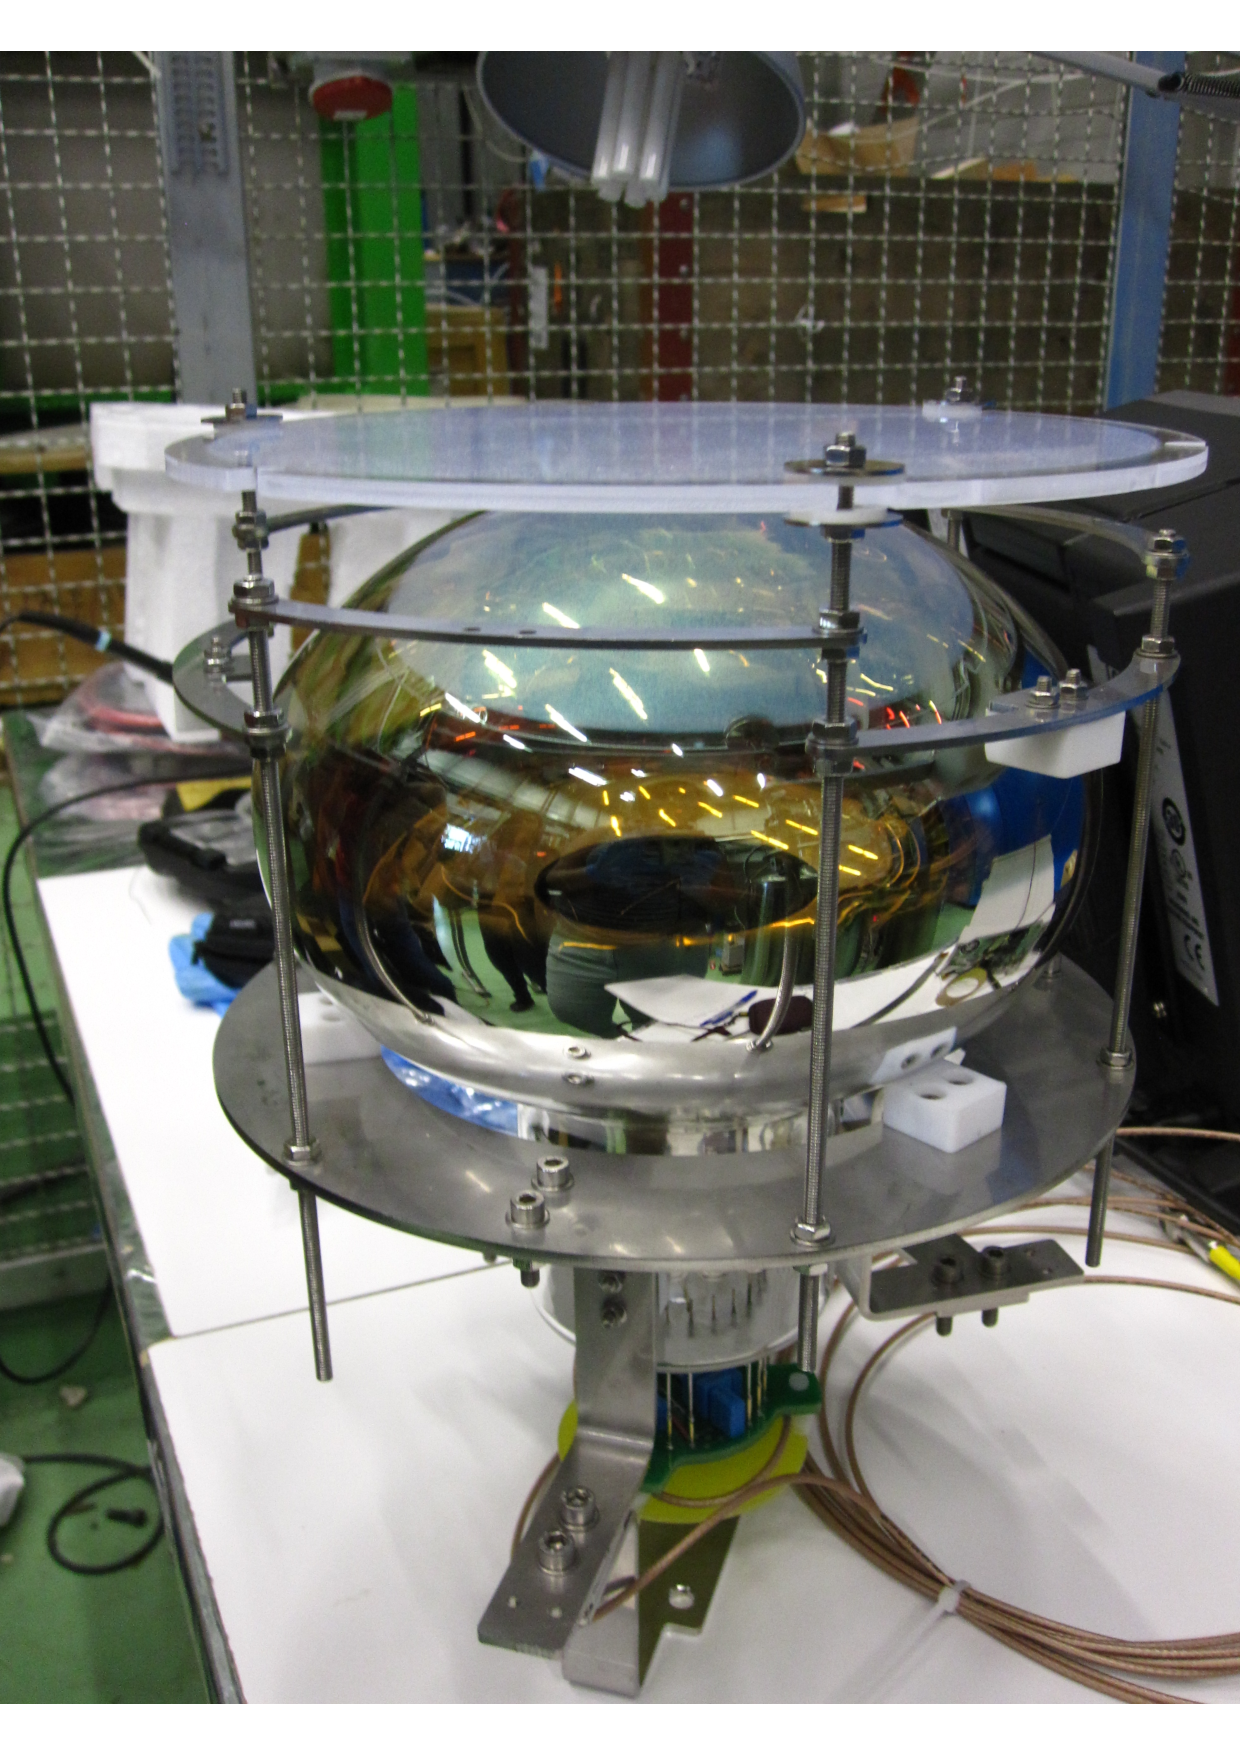
\includegraphics[width=0.25\textwidth]{graphics/dppd_PMTPlate}
%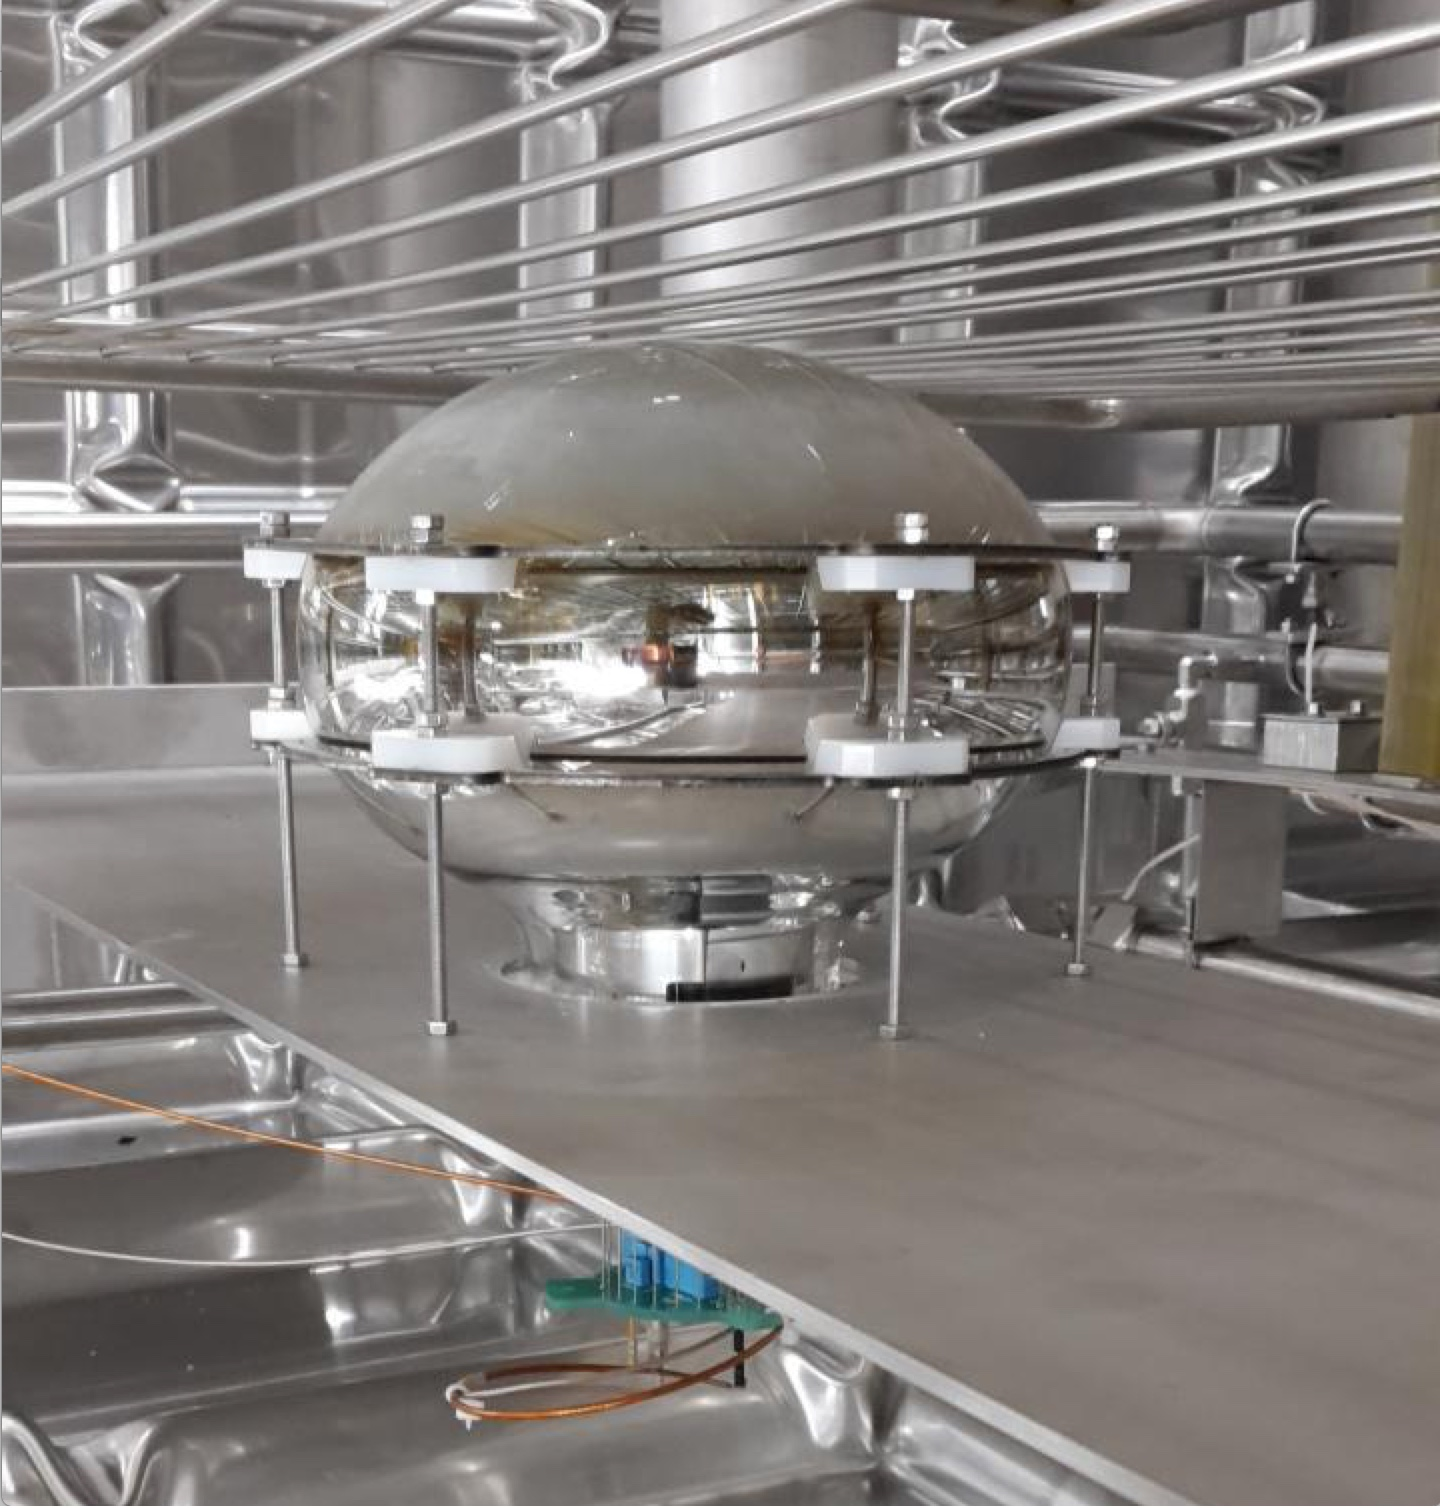
\includegraphics[width=0.33\textwidth]{graphics/dppd_PMTTPB.jpeg}\\
%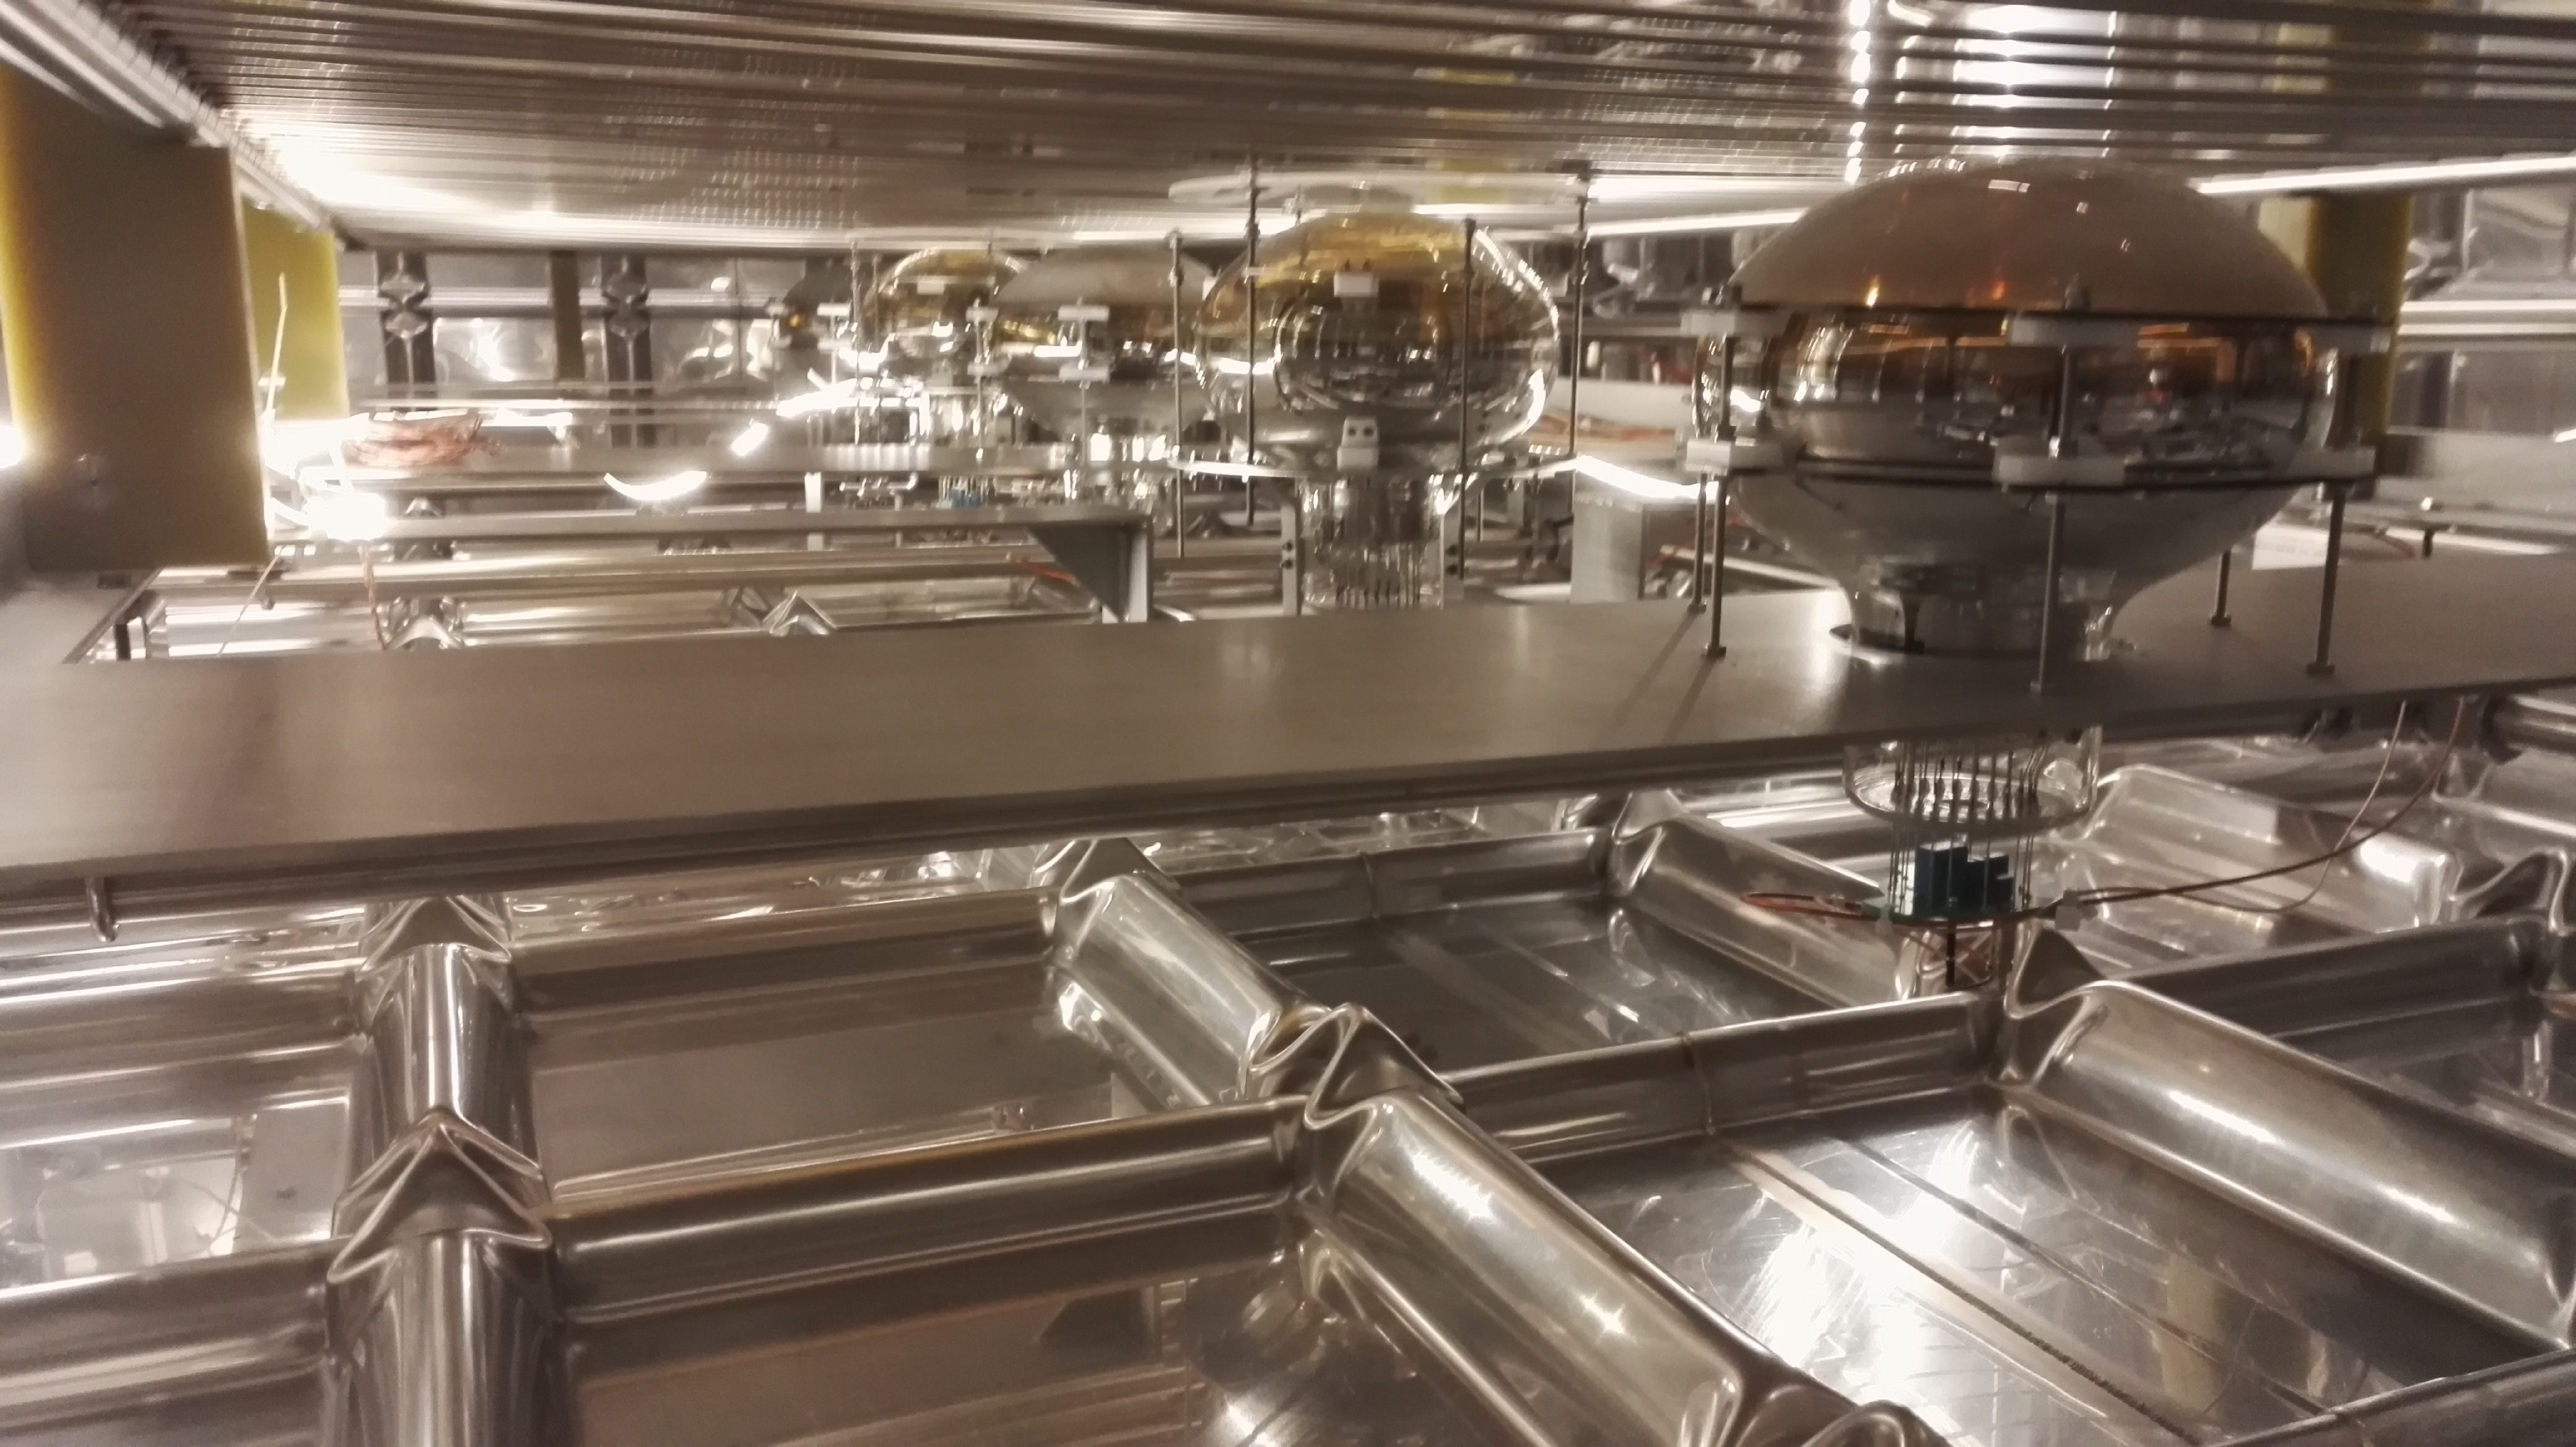
\includegraphics[width=0.6\textwidth]{graphics/dppd_PMT_311_installation.jpg}
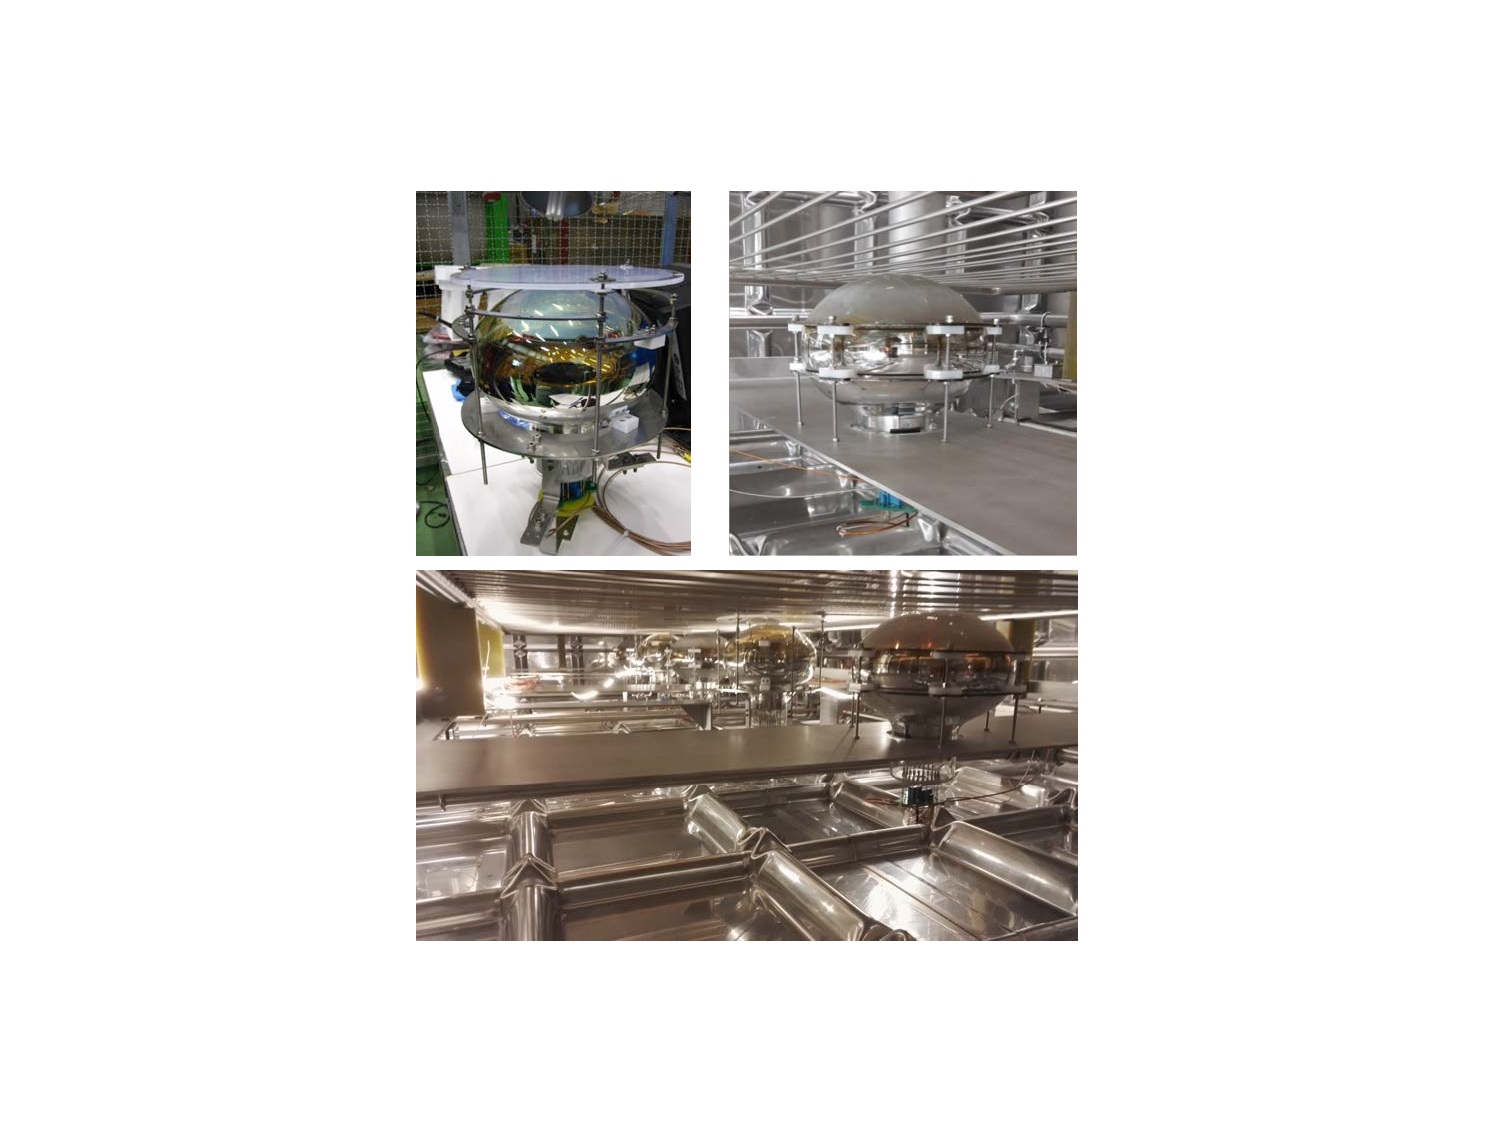
\includegraphics[width=0.5\textwidth]{dppd_311_PMT_combined}
\end{dunefigure}

Two power supply polarities were used. Three \dwords{pmt} were equipped with a negative \dword{hv} base, i.e. a negative bias voltage was applied to the photocathode, and the anode was grounded. This system requires two cables: one for the \dword{hv} system and one for the signal. A positive base served the other two \dwords{pmt}: a single cable positively biased the anode and carried the signal, and the cathode was grounded. The \dword{hv} and the signal were then externally decoupled using a splitter, see Section~\ref{sec:fddp-pd-4.2}. The latter design has the advantage of reducing the number of feedthroughs and cables while also reducing the noise. Overall, four configurations were tested (see Table~\ref{tab:dp-pds-311conf}). During the 3$\times$1$\times$1~m$^3$ operation, the \dwords{pmt} operated at a rather uniform gain of around \num{e6} with a readout sampling of \SI{250}{MHz}.

\begin{dunetable}
[\dshort{wa105} \dshorts{pmt} configurations.]
{cccccc}
{tab:dp-pds-311conf}
{Configuration of the five \dwords{pmt} installed in the \dword{wa105}.}
\dword{pmt} & Base & Coating & Voltage (kV) & Gain (\num{e6}) & Noise (ADC)\\
%\hline
1 & Negative & Coating & \num{-1.2} & 0.92$\pm$0.13 & \num{0.7} \\
2 & Negative & Plate   & \num{-1.2} & 1.01$\pm$0.12 & \num{0.7} \\
3 & Positive & Coating & \num{1.1} & 0.95$\pm$0.11 & \num{0.4} \\
4 & Positive & Plate   & \num{1.1} & 1.26$\pm$0.15 & \num{0.4} \\
5 & Negative & Coating & \num{-1.2} & 1.33$\pm$0.15 & \num{0.8} \\
%\hline
\end{dunetable}

In \dword{pddp}, \num{36} \dwords{pmt} are installed \SI{6}{\m} below the collection plane, again underneath the cathode and the \dword{gg}. The \dword{pmt} density is lower than the demonstrator. Their positioning over the \SI{36}{m$^2$} area was optimized with simulations. The number of \dwords{pmt} is higher around the center of the active volume and lower near the \dword{fc} borders. This positioning maximizes the amount of light collected from cosmic rays.

After evaluating the demonstrator configurations, the \dword{tpb} was directly evaporated onto the \dword{pmt} windows, and the \dword{pmt} base was chosen to have positive polarity. This configuration maximizes collection efficiency and reduces both the number of cables and the electronic noise. 

For \dword{dune} \dword{fd} \dword{pds}, \dword{tpb} will be directly applied to the \dword{pmt} windows, and the positive biasing scheme will be implemented. The aspect ratio between cathode size and drift distance is larger than in \dword{pddp}, so the amount of light loss by absorption on the \dword{fc} should be smaller. Therefore, the \dword{dune} \dword{fd} \dword{pds} layout should be uniform with \dwords{pmt} on a regular lattice with \SI{1.02}{m} spacing. 

%%%%%%%%%%%%%%%%%%%%%%%%%%%%%%%%%%%%%%%%%%%%%%%%%%%%%%%%%%%%%%%%%%%%

\subsection{\dshort{wa105} Light Data Results and Simulation Validation}

Analysis of data taken during the \dword{wa105} operation provides the first validation of and improvements in the light simulation developed so far. 
The demonstrator ($3\times1\times1$~m$^3$ active volume) has linear dimensions comparable with the Rayleigh scattering length, which is approximately \SI{60}{\cm}. 
As a consequence, the light absorbed by elements of the detector (such as the \dword{fc}, \dword{lem}, or cathode) may become a problem.
Hence, light maps were created with particular care for precision in reproducing the demonstrator's geometry.

Two triggering schemes were used during the \dword{wa105} operation.
The first was provided by an external muon tagger, the \dword{crt}, to record horizontal muons. The \dword{crt} was made of plastic scintillator planes on each side of the detector.
The second was provided by the \dwords{pmt} themselves, requiring that the five sensors record sufficient light in coincidence. In this configuration, more vertical muons and showers were recorded.

Using the \dword{crt} trigger condition, a rough track reconstruction is possible because the \dword{crt} provides coordinate information with \SI{11}{\cm$^2$} resolution. Hence, even without charge information, as for data taken at null field, it is possible to select muon-like tracks and retrieve the shortest distance between the track and each \dword{pmt}. A schematic drawing of the \dword{wa105} detector is presented in Figure~\ref{fig:pd-pds-311schema} with the relevant track parameters.

\begin{dunefigure}[\dshort{wa105} schematic drawing]{fig:pd-pds-311schema}{Schematic view of the \dword{wa105}. 
The fiducial volume is in gray and limited from the collection plane area to the cathode. The active volume is in yellow. Its volume is defined by the collection plane: the \dword{fc} to the top of the \dwords{pmt}. A track that would be detected by the \dword{crt} is shown with its minimum distance to \dword{pmt} \num{3} in red.}
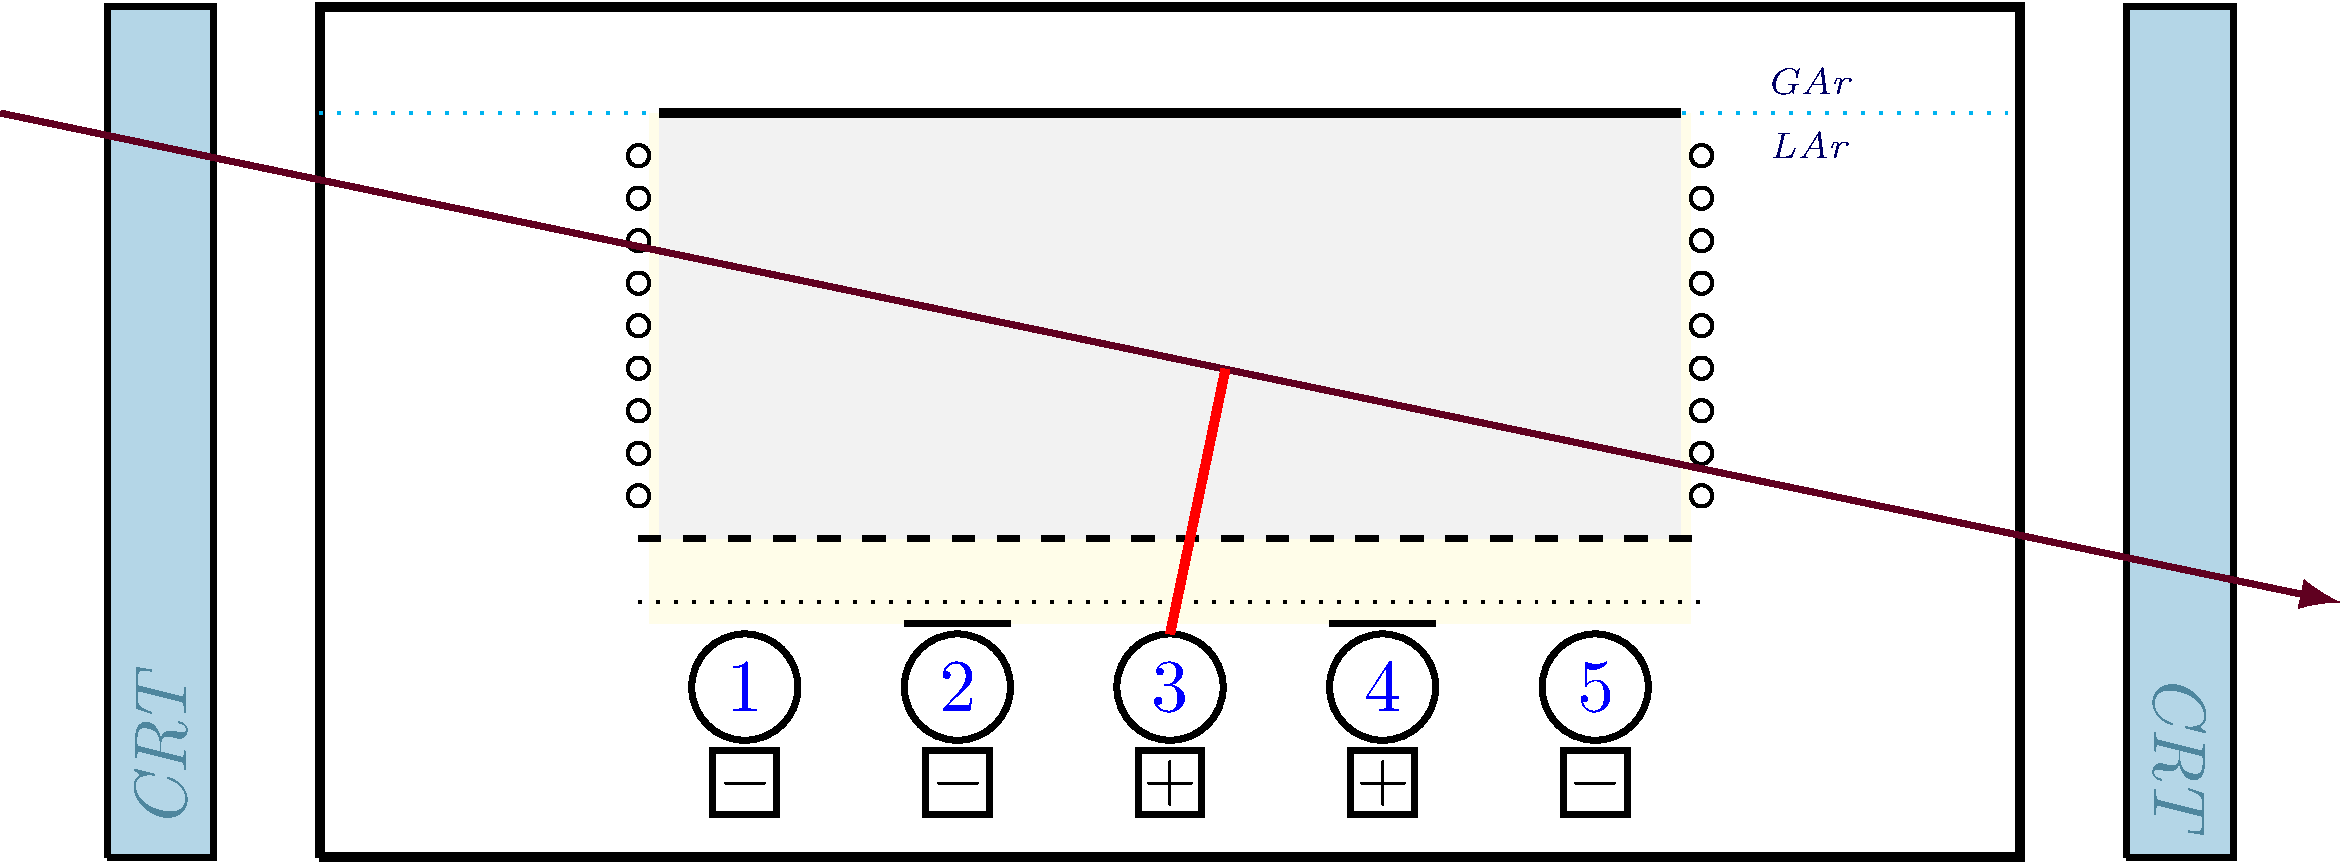
\includegraphics[width=0.75\textwidth]{graphics/dppd_7_2_v2}
\end{dunefigure}

From the \dword{pds} point of view, the \dword{wa105} operation lasted several months because light was collected during cool down, filling, and commissioning stages of the demonstrator.
The \dword{pds} performed with high stability during this entire period. 
In Figure~\ref{fig:pd-pds-311-ped}, the  pedestal \dword{rms} is shown for one positive and one negative base \dword{pmt} as a function of time for \num{5} months of operation. 

\begin{dunefigure}[\dshort{wa105} \dshort{pmt} pedestal \rms]{fig:pd-pds-311-ped}{Pedestal \dword{rms} for one negative base \dword{pmt} (black) and one positive base \dword{pmt} (red) between July and December 2017 during the operation of the \dword{wa105}.}
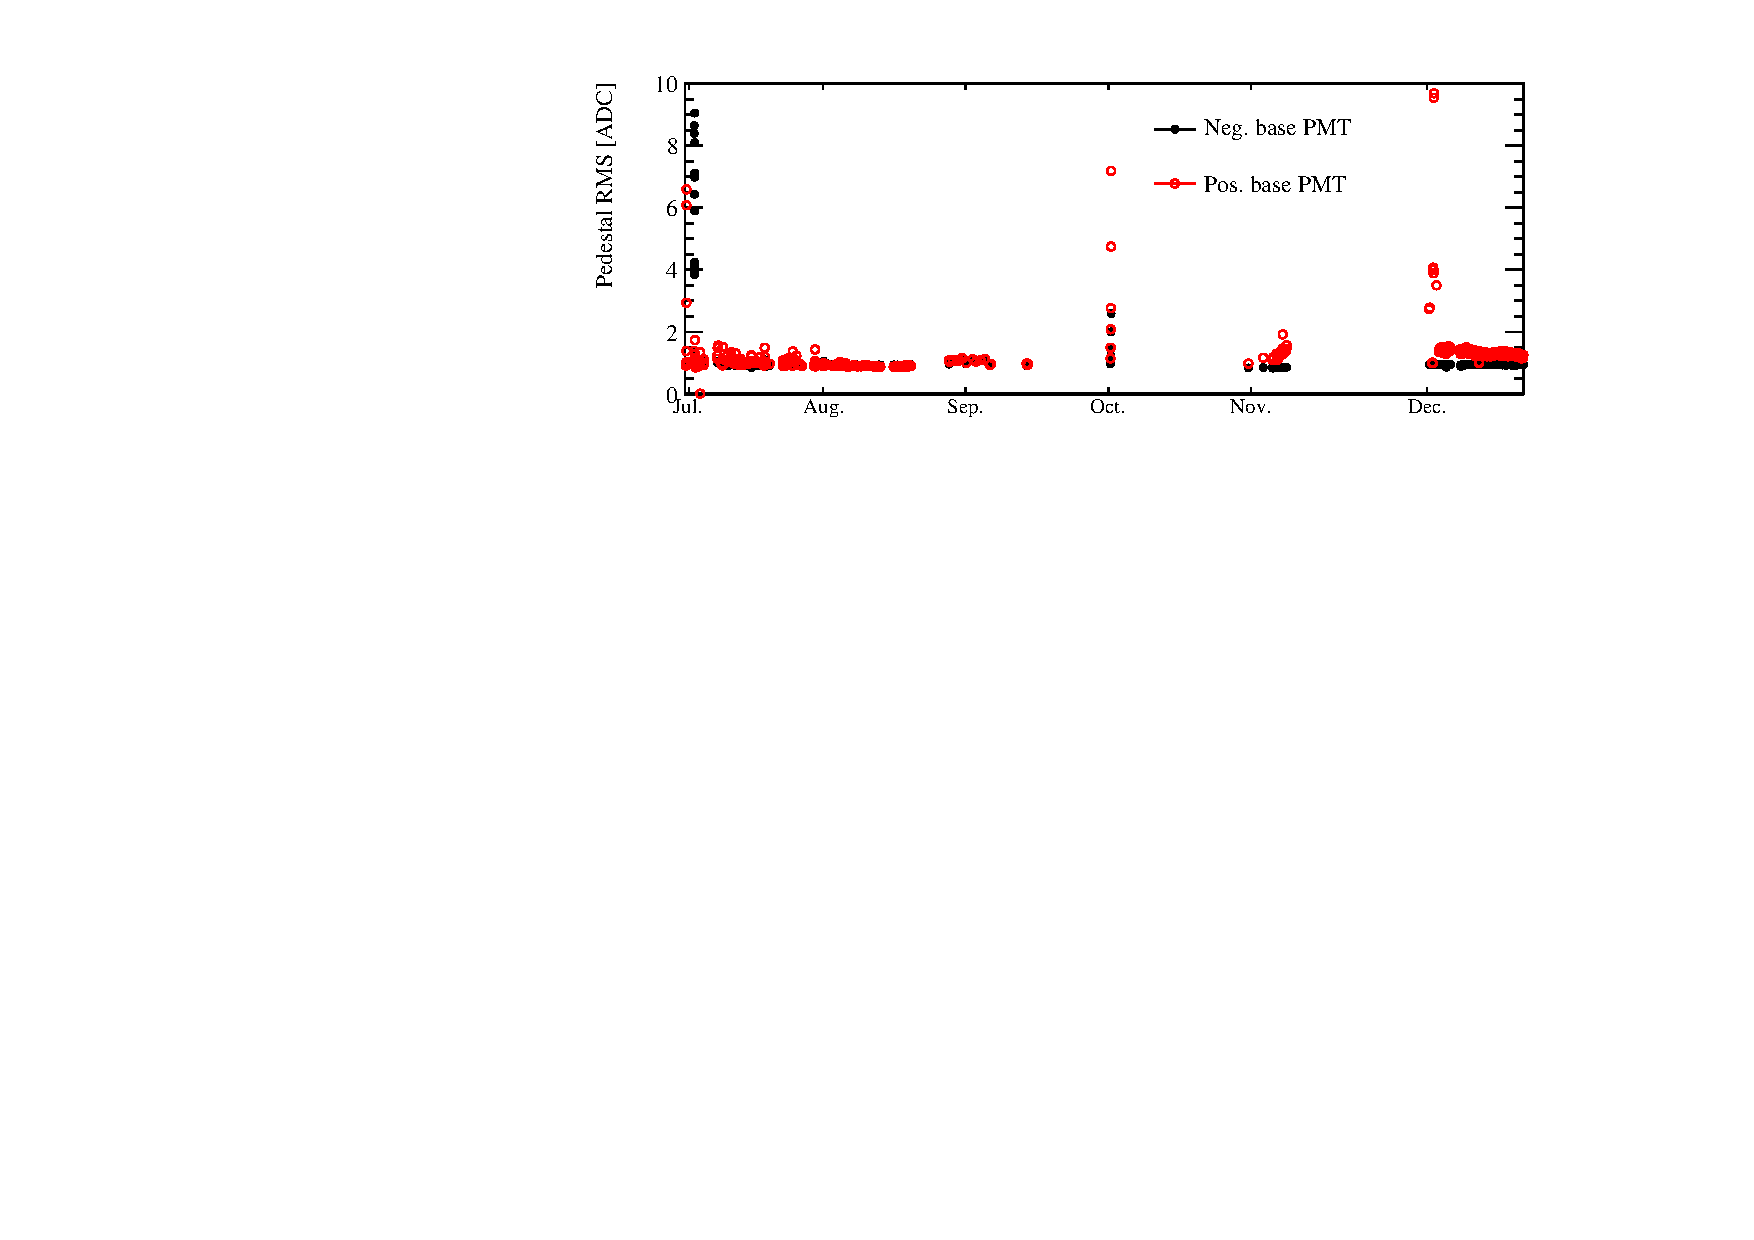
\includegraphics[width=0.9\textwidth]{graphics/dppd_311_pedestal_rms.pdf}
\end{dunefigure}

Figure~\ref{fig:pd-pds-311-LAr-GAr} shows the average waveforms for \dword{pmt} 5 in gas and liquid argon with no drift field. These waveforms are fitted with a gaussian to describe the response function convoluted with a sum of three exponentials to describe the fast, slow, and intermediate components. 
The extracted values agree with the literature, although the lifetime of the fast component has been fixed at \SI{6}{ns} in the fitting procedure.

\begin{dunefigure}[GAr and LAr scintillation profile in \dshort{wa105}]{fig:pd-pds-311-LAr-GAr}{Scintillation time profile in the absence of drift field recorded in GAr (left) and LAr (right) in black. In red, the fit performed with a sum of 3 exponentials (describing the fast, intermediate, and slow components, all shown as dotted blue lines) convoluted with a gaussian to take into account the response function of the \dword{pmt}. The intermediate component improves the fit quality considerably although a consensus on its interpretation is not reached in the community at this moment. The extracted lifetimes are shown in the figure.}
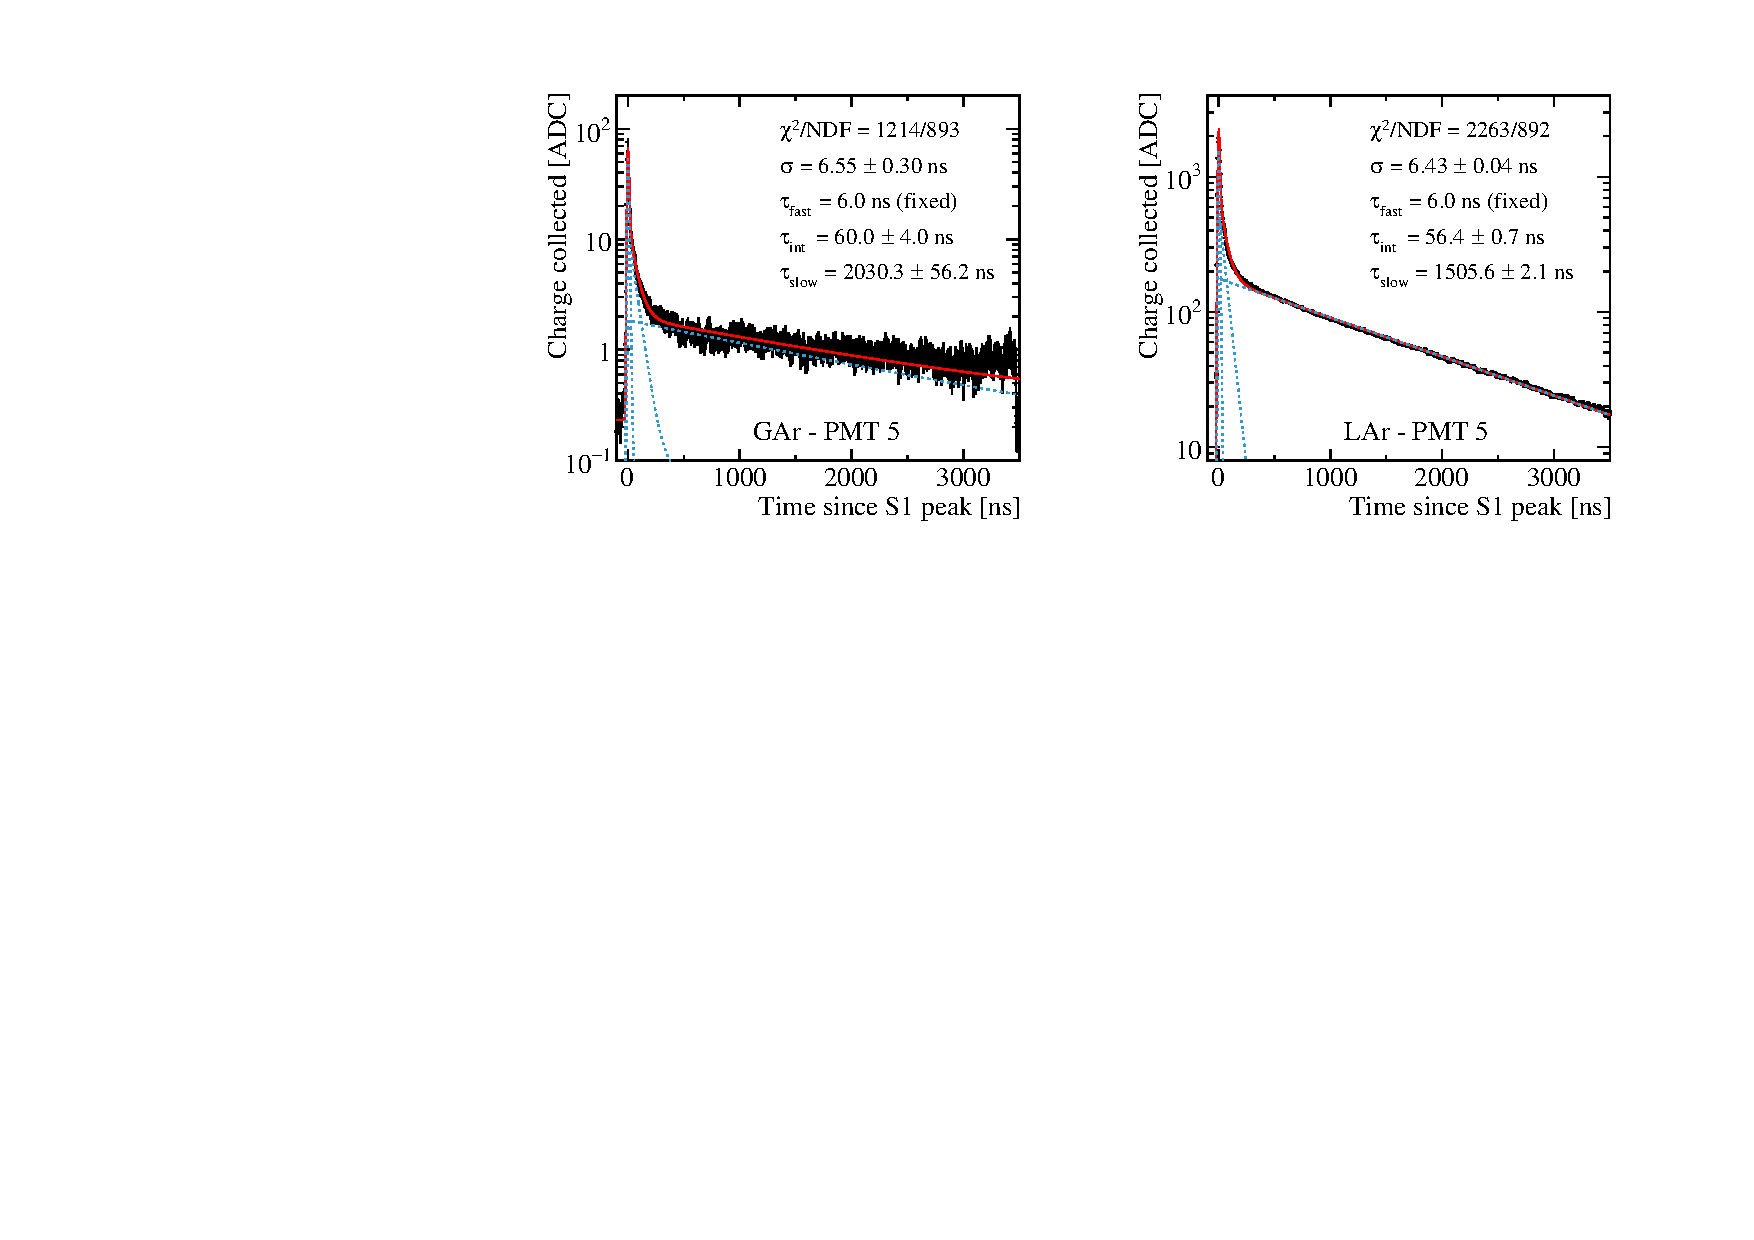
\includegraphics[width=0.85\textwidth]{graphics/dppd_311_lar_gar_fit.pdf}
\end{dunefigure}

Many studies show that $\tau_{slow}$, the slow component (Section~\ref{sec:dp-pds-overview_scintillation}) is very sensitive to the amount of impurities in the liquid.
To monitor the purity of the liquid argon as a function of time, the same fit has been performed on several runs under similar conditions. 
Figure~\ref{fig:pd-pds-311-purity} presents the evolution of $\tau_{slow}$ for \SI{15}{days} of operation.
The results exhibit a very stable amount of impurities, which agrees with the stability of the electron lifetime measured using the charge collection.

\begin{dunefigure}[Evolution of $\tau_{slow}$ as a function of time in \dshort{wa105}]{fig:pd-pds-311-purity}{Evolution of $\tau_{slow}$ over \num{15} days of operation of the \dword{wa105}. The points are the averages over the values extracted from the fits to the waveforms of the \num{3} negative base \dwords{pmt} for runs taken with no drift field. Preliminary results.}
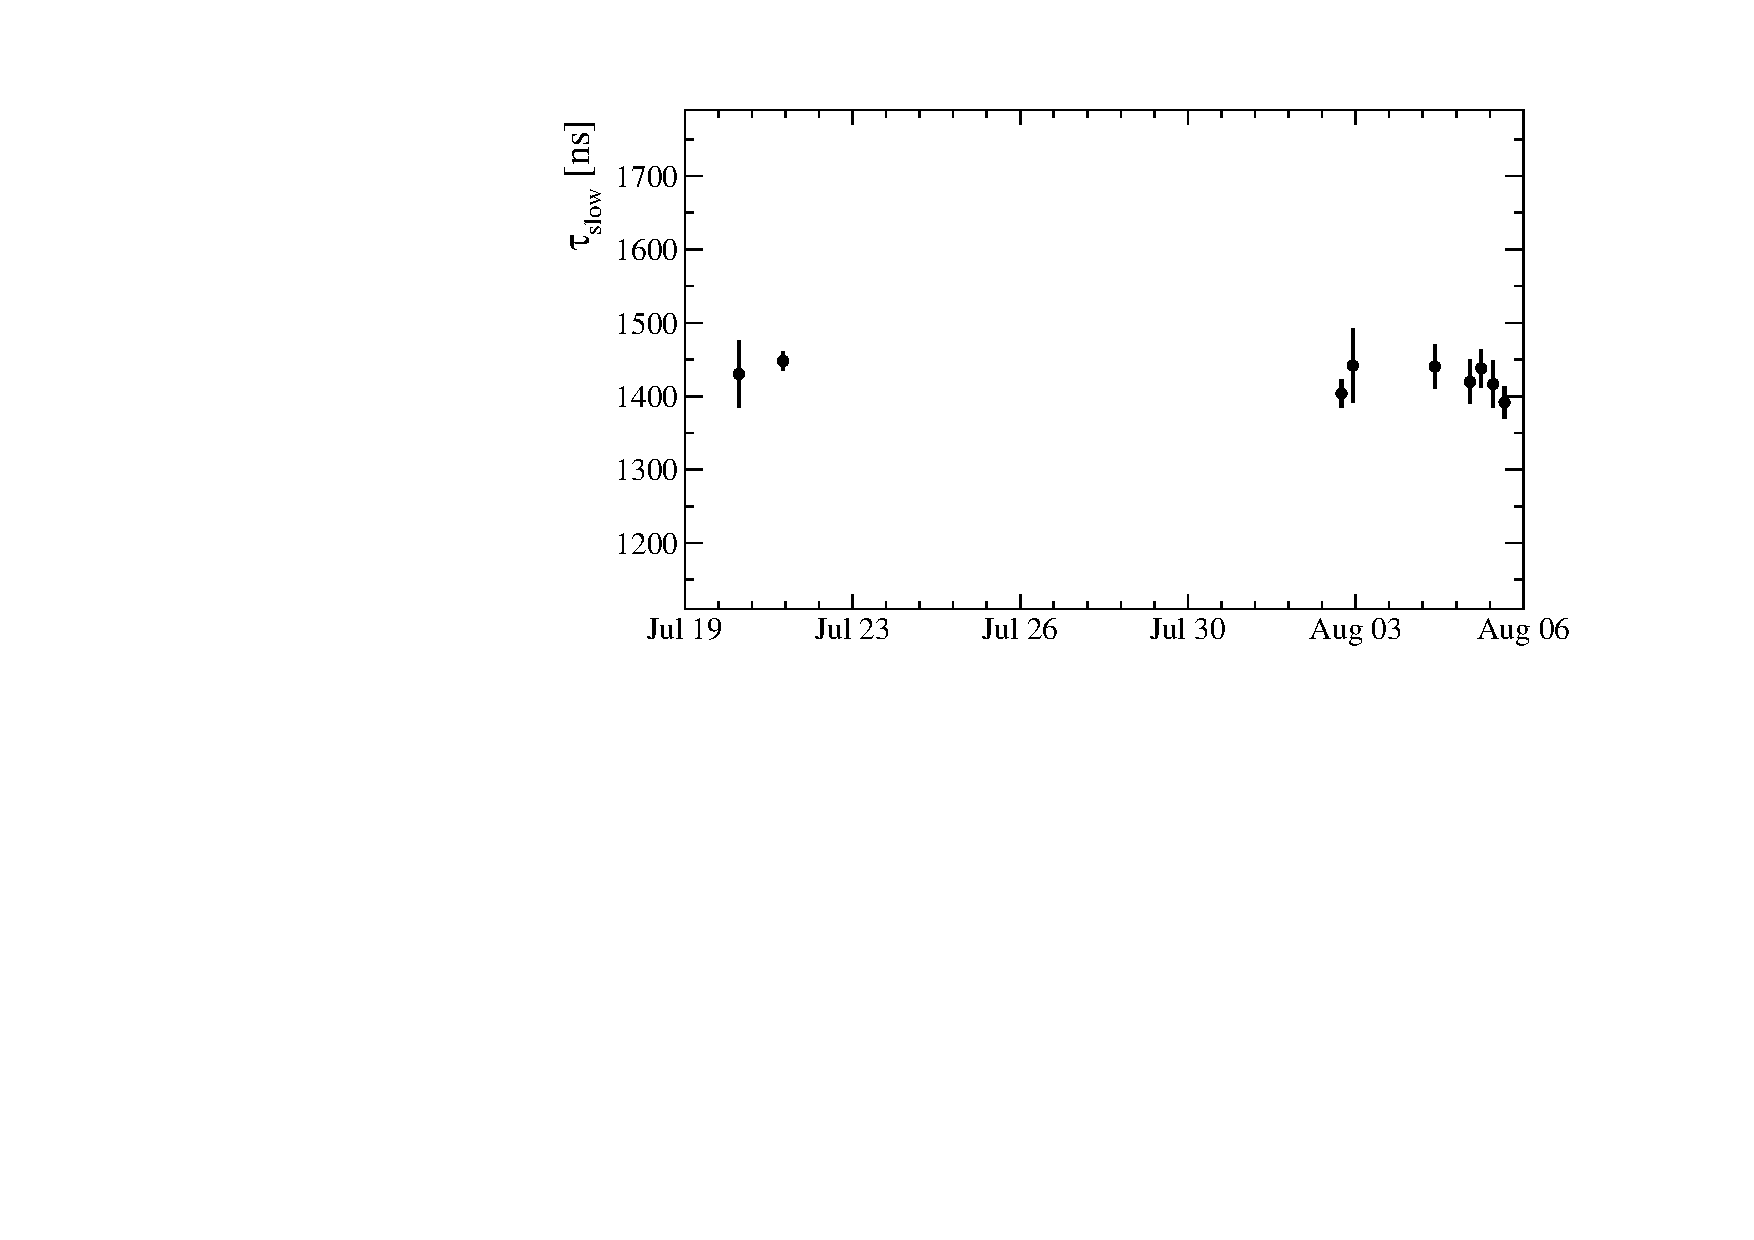
\includegraphics[width=0.7\textwidth]{graphics/dppd_311_purity.pdf}
\end{dunefigure}

The S2 light has also been recorded in dedicated runs using a \SI{1}{ms} recording time window.
Figure~\ref{fig:pd-pds-311-S2} shows the average waveforms from runs with a drift field of \SI{0.5}{kV/cm} and an extraction field of \SI{2}{kV/cm} (\SI{3}{kV/cm}) in liquid (gas). In the figure, one run has no amplification field, the others have the \dwords{lem} polarized to provide an amplification field of \SI{25.5}{kV/cm}. 
The effect of the \dwords{lem} on the amount of S2 light generated is clear. 
The S2 light extends for about \SI{600}{$\mu$s} after emission of the prompt signal, agreeing with the electron drift time over \SI{1}{m} in such drift field.

\begin{dunefigure}[S2 light at different amplification field in \dshort{wa105}.]{fig:pd-pds-311-S2}{Average waveforms of negative based \dwords{pmt} in a \SI{1}{ms} window. Both runs were taken with a drift field of \SI{0.5}{kV/cm} and an extraction field of \SI{3}{kV/cm} in gas. The S2 light extends for about \SI{600}{$\mu$s}, as expected.}
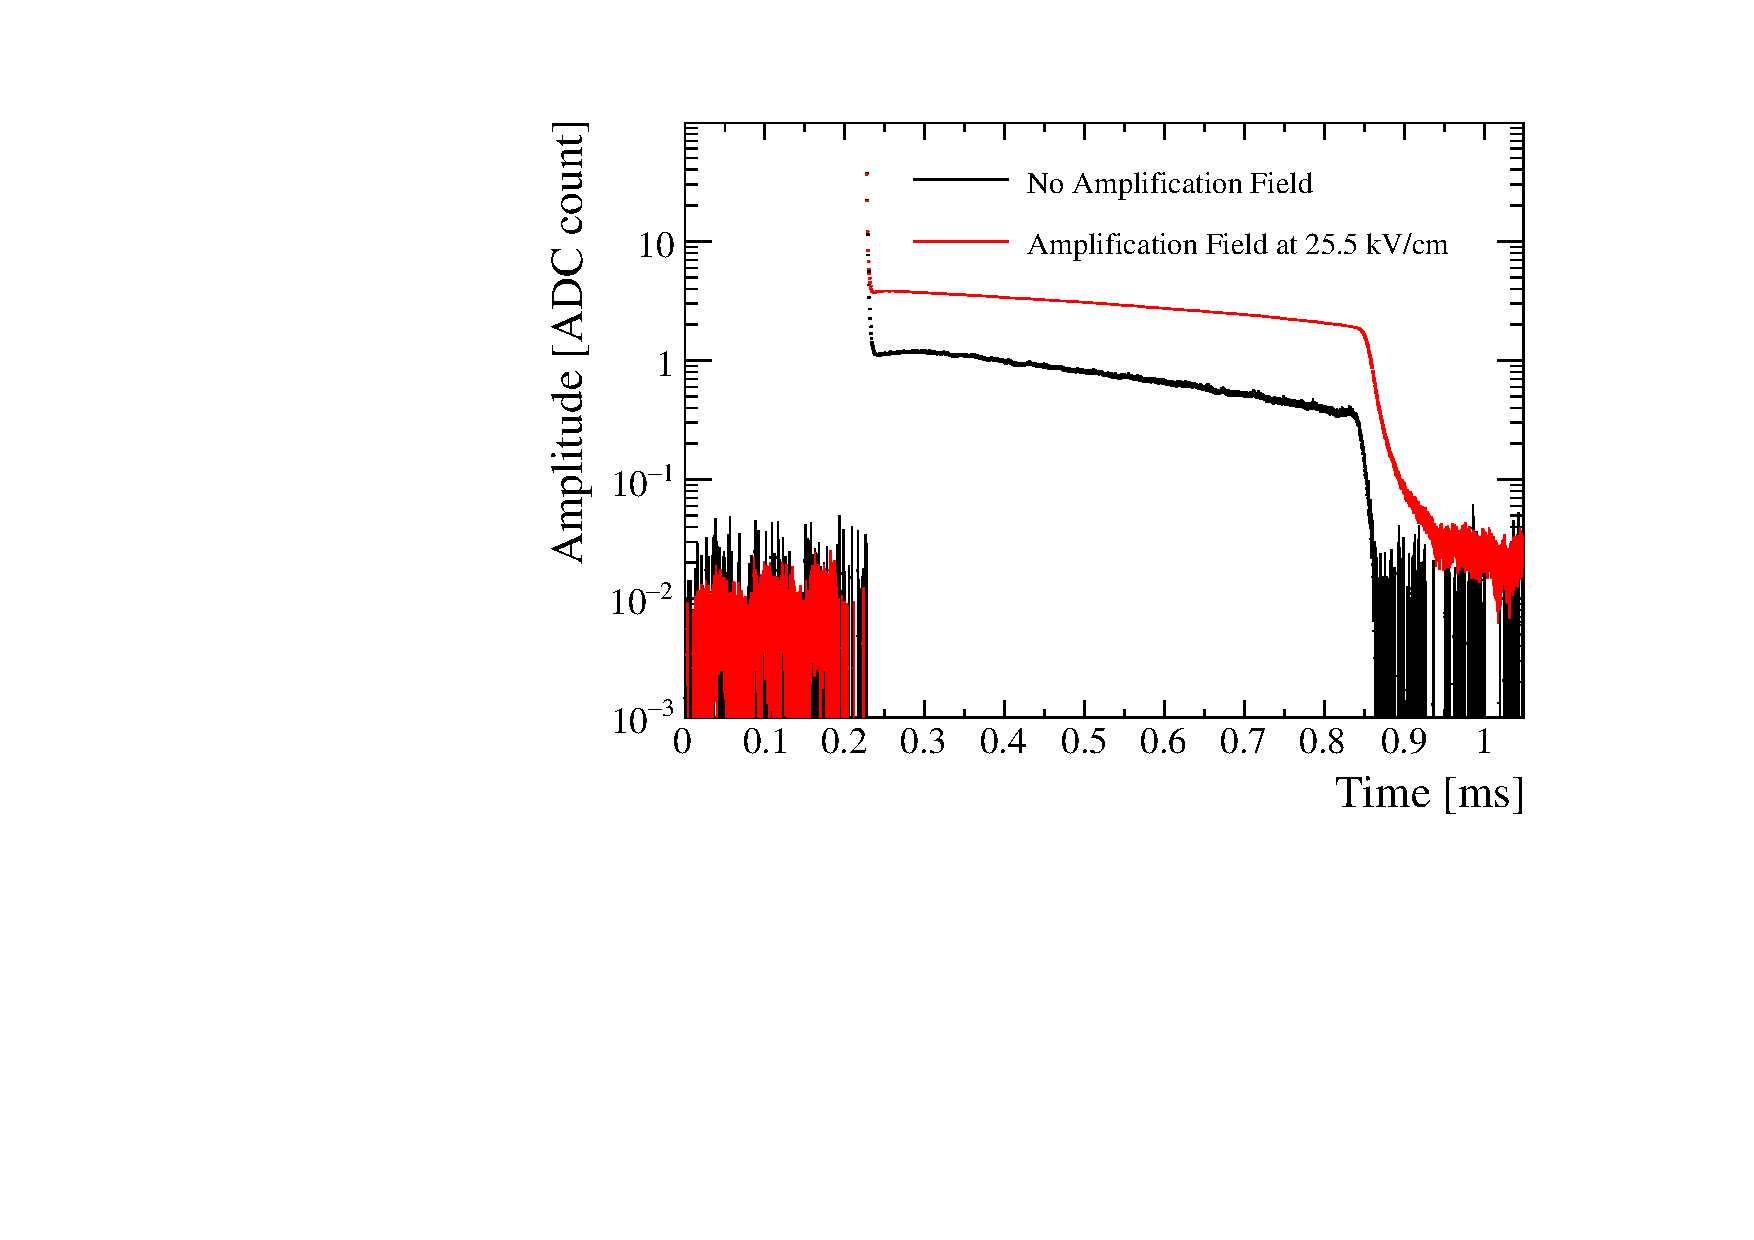
\includegraphics[width=0.7\textwidth]{graphics/dppd_311_S2_extraction.pdf}
\end{dunefigure}
Using data taken at null field in \dword{crt} triggering mode, muon-like tracks are selected. Further, the tracks must cross the active volume for distances longer than \SI{3.1}{\m}. 
The S1 charge collected by each \dword{pmt} is calculated by integrating the \dword{adc} values in a \SI{1}{\us} window starting from the S1 peak; this charge value is then converted into the number of detected \dwords{pe} using the calibrated \dword{pmt} gains in Table~\ref{tab:dp-pds-311conf}.

In the simulation, \SI{4}{\GeV} muons are generated from one \dword{crt} panel to the other with data-driven kinematics. The number of PEs collected by each \dword{pmt} is generated according to the light maps. To suppress spurious triggers, data analysis uses a selection of the minimum amount of light recorded by all \dwords{pmt}; this does not apply to \dword{mc}. Moreover, the \dword{pmt} signal must not saturate the readout only for data analysis, but not \dword{mc}. Figure~\ref{fig:dp-pds-311charge} compares the number of PEs collected in data analysis and in \dword{mc}. The data and \dword{mc} agree well with one another. 

In the \dword{wa105}, the \dword{pmt} gain was adjusted so S1 and S2 light could be seen and thus increase the trigger rate while minimizing the \dword{pmt} \dword{adc} saturation. 
In \dune \dual, the situation will be different as the volume is much larger and part of the triggering modes will be independent from the \dwords{pmt}. 
Hence the \dword{pmt} gain will be adjusted accordingly and the events saturating the ADC should not be as problematic as it could be in \dword{wa105}.
%\fixme{Give more details about why \dword{pmt} saturation in \dword{wa105}, and why this is not worrisome in \dpmod?}

\begin{dunefigure}[Charge collected in \dshort{wa105} vs \dshort{mc}]{fig:dp-pds-311charge}{ Charge collected by the \dwords{pmt} in a \SI{1}{\us} window containing the S1 peak for muon-like tracks triggered by the \dword{crt} panels. The data is shown in black and the simulation in red. The distributions are normalized to unity for clarity. Preliminary results.}
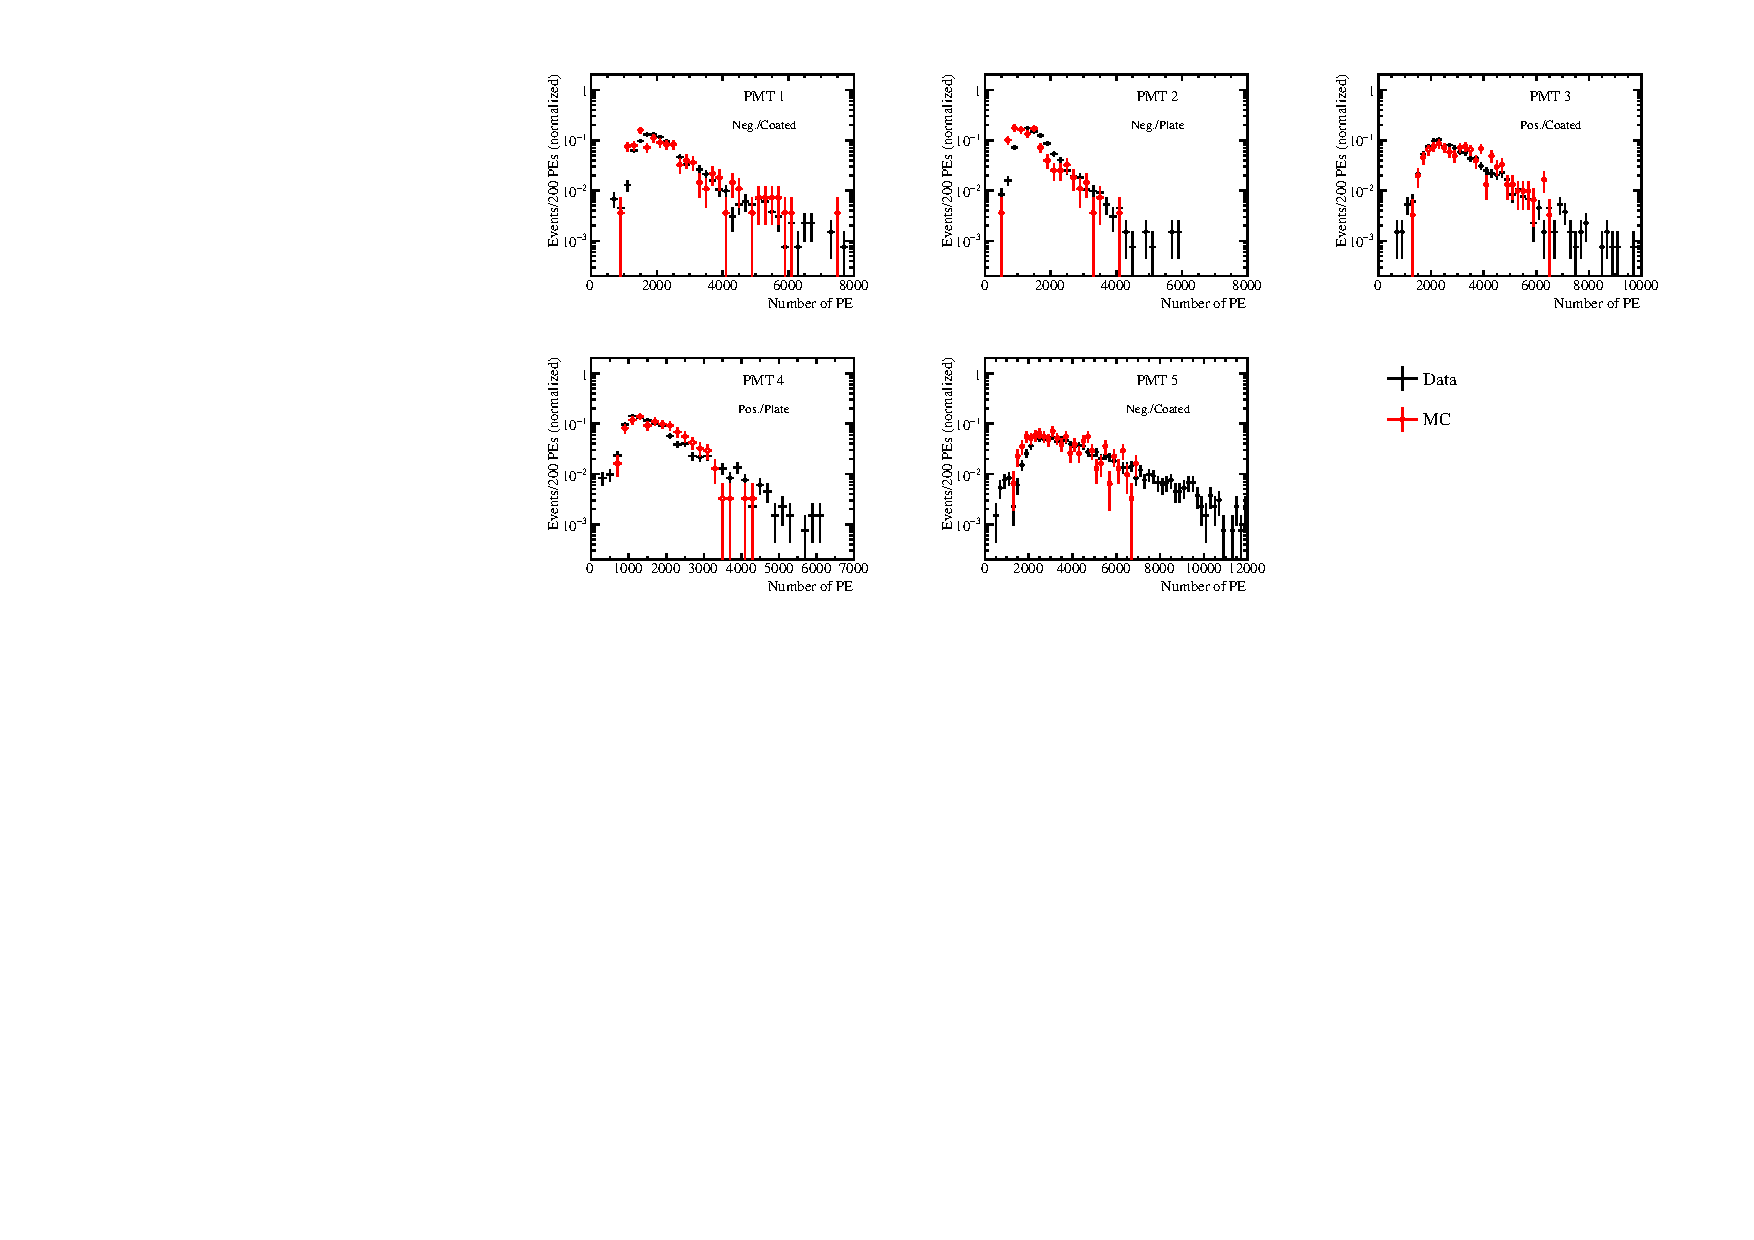
\includegraphics[width=0.95\textwidth]{graphics/dppd_311_charge_mc_v2.pdf}
\end{dunefigure}

\begin{dunefigure}[Charge collected vs track-PMT shortest distance]{fig:dp-pds-311profile}{Profile histograms of charge collected as a function of the track-PMT shortest distance. The data is in black, the simulation in red. Preliminary results.}
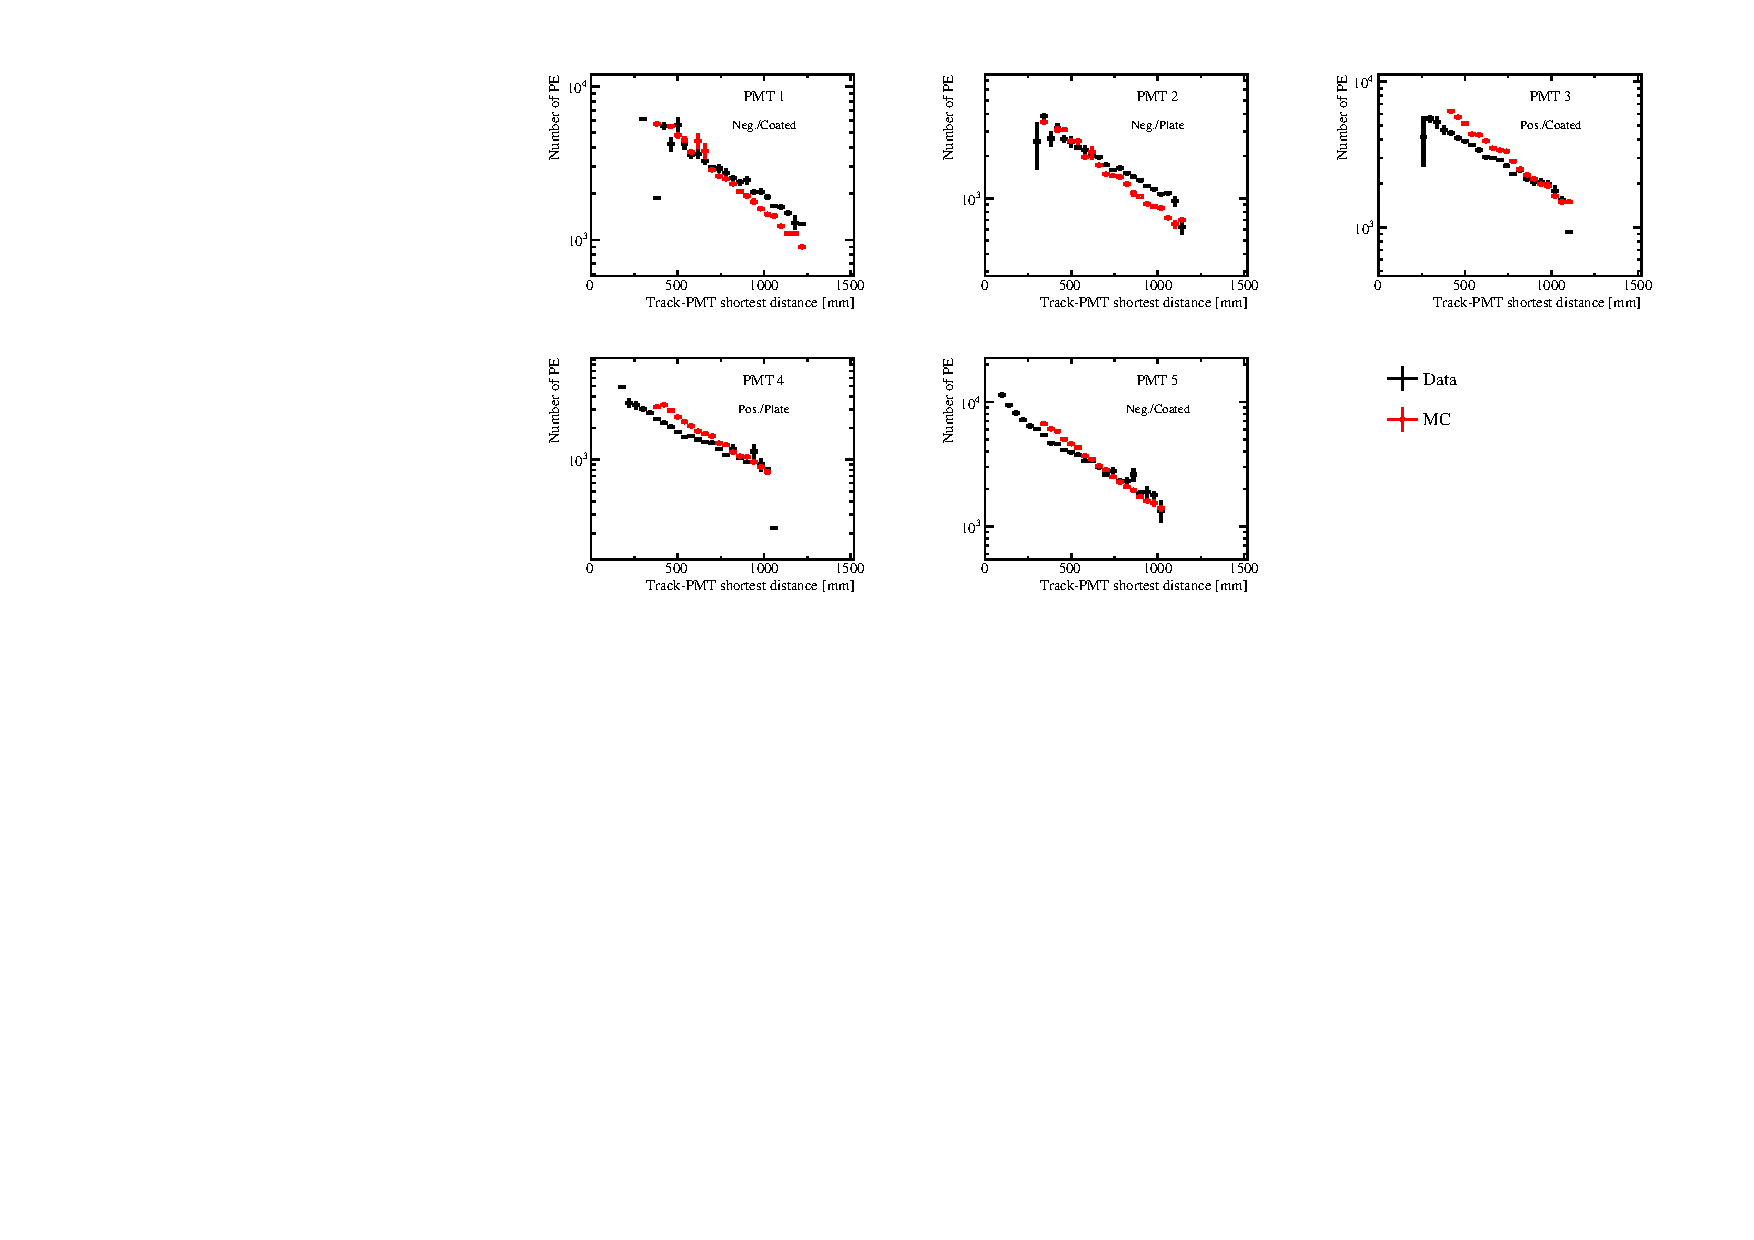
\includegraphics[width=0.95\textwidth]{graphics/dppd_311_charge_dist_mc.pdf}
\end{dunefigure}

%\fixme{This is rather distance vs charge. Is it possible to swap the x and y axis and reproduce the plots?}

The \dwords{pe} collected per \dword{pmt} depends strongly on the shortest track-\dword{pmt} distance. Many factors can affect how much charge is collected, primarily, the scattering length, also known as the Rayleigh scattering length. This quantity is still subject to debate among the \dword{lar} community because its measurement is fairly complicated. Current estimates of the scattering length range from \SI{20}{\cm} to \SI{1}{\m}.
In the \dword{wa105} simulation, the scattering length was set to L$_{ray}$ = \SI{55}{\cm}.
Figure~\ref{fig:dp-pds-311profile} shows the charge collected as a function of the shortest track-\dword{pmt} distance in the form of profile histograms. The overall trend is very similar for data and \dword{mc}, also across all the \dwords{pmt}. However, the profile histogram slopes indicate that the assumed scattering length in \dword{mc} could be better tuned to reproduce the data, e.g., toward larger values of the Rayleigh scattering length.

%%%%%%%%%%%%%%%%%%%%%%%%%%%%%%%%%%%%%%%%%%%%%%%%%%%%%%%%%%%%%%%%%%%%

\subsection{Installation of the \dshort{pddp} Photon Detector System}

At the time of writing, no scintillation light data from \dword{pddp} are yet available. Nevertheless, important lessons from \dword{pddp} have already been learned, thanks to the recent installation of its photon detector system. They are summarized below. Figure~\ref{fig:dppd_pmt_installation} shows the placement of the \num{36} \dwords{pmt} in \dword{pddp} on the cryostat floor, performed in February 2019.

\begin{dunefigure}[Installation of the \dshort{pddp} PDS]{fig:dppd_pmt_installation}{Installation of the \dword{pddp} photon detector system.}
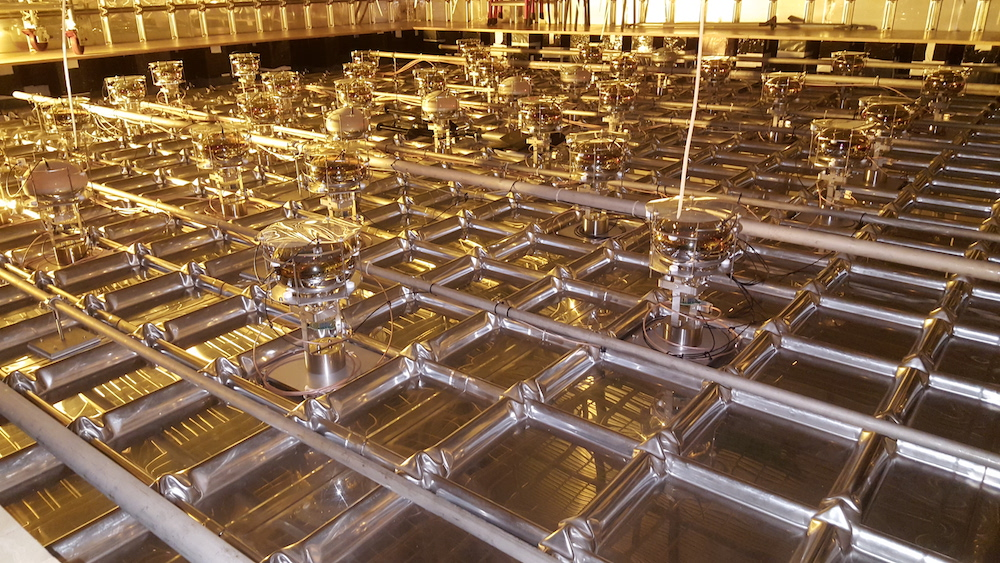
\includegraphics[width=0.8\textwidth]{graphics/dppd_pmt_installation.jpg}
\end{dunefigure}

One of the most critical points of the installation is the order of the tasks. Since the installation activities lasted several days in the \dword{pddp} case, and will last several months for an \dword{fd} module, and given that other persons have to work near the \dword{pds} components, the risk of damage has to be considered. The fragility of the components determines the installation order. The \dword{pmt} supporting bases and the signal-HV \dword{pmt} cables must be be installed first, then the \dwords{pmt} can be mounted on their holders and connected to the cables, and finally the calibration fiber system has to be installed. The need of protecting the components has to be evaluated if there are subsequent activities around them. For example, Figure~\ref{fig:dppd_pmt_installation} shows how temporary protective plates were placed in front of the \dword{pddp} \dword{pmt} photo-cathodes, and the \dword{pmt} units were enclosed in temporary plastic bags. 

The conceptual division of the \dword{fd} \dword{pds} into several sectors is crucial. In \dword{pddp}, the \num{36} \dwords{pmt} were divided into six groups of \num{6} \dwords{pmt} each. This arrangement simplified the installation of the calibration fibers considering that each fiber bundle has \num{7} fibers, including one spare fiber per bundle. 

Concerning organizational matters, \dword{pddp} experience shows that several documents should be prepared prior to installation, including a detailed description of all the tasks to be performed, a time estimation for all of them, and a list of the necessary items. In addition, the required status of the detector before each installation stage should be indicated. This information must be as detailed as possible. The benefits of a detailed planning are:

\begin{itemize}
\item All the persons participating in the \dword{pds} installation know their roles.
\item The required material is foreseen and available when needed.
\item The interaction with other installation crews is planned.
\item The expected time for the installation is known in advance and extra time for unexpected events can be added.
\item It is possible to communicate beforehand all the requests to the coordinator of the installation.
\item The overlapping of activities and the waiting times are minimized. 
\end{itemize}

\section{Baseline Design Validation and Projected Photon Detector Performance}
\label{sec:dp-pds-performance}

After the initial simulation studies described in the \dword{fd} \dword{tp}~\cite{Abi:2018rgm}, we have progressed toward a more realistic understanding of the projected \dword{pds} performance using the \dword{larsoft} framework:
%
\begin{itemize}
\item Optical simulations are now performed in the \dword{dpmod} geometry. In the  \dword{tp}, physics studies assumed the \dword{pddp} geometry. Considering the lack of any optical segmentation in the \dword{dp} design, light is simulated in the full \dword{tpc} active volume. Simulation assumptions for light generation and light transport are described in Section~\ref{subsec:dp-pds-simulation_assumptions}. 
%
\item The electronics response and the reconstruction of optical hits and optical clusters has been simulated. Simulation assumptions for light detection by the \dwords{pmt} are also described in Section~\ref{subsec:dp-pds-simulation_assumptions}. Optical hits are the reconstructed optical signals on single \dword{pmt} waveforms and are characterized by a hit time, amplitude, and charge. Optical hits must have an amplitude of at least \SI{10}{ADC counts} above baseline. Optical clusters refer to a collection of \dword{pmt} hits correlated in time and space. They are typically induced by the same underlying flash of scintillation light in \dword{lar}. The parameters of the clustering algorithm are discussed later in this section.

%
\item The physics studies now also include radiological backgrounds. Simulating radiological backgrounds is critical in realistically optimizing the optical reconstruction parameters. The radiological model includes several radio-isotopes throughout the \dword{lar} volume, with \SI{1.01}{\becquerel/\kg} of $^{39}$Ar providing the most activity. In addition, the model accounts for an impinging neutron flux of \SI{e-5}{\cm$^{-2}$\s$^{-1}$}. % is accounted for.
\end{itemize} 

The expected \dword{pds} light yield in the \dword{dp} \dword{fd} module geometry is discussed in Section~\ref{subsec:dp-pds-simulation_yields}

%%%%%%%%%%%%%%%%%%%%%%%%%%%%%%%%%%%%%%%%%%%%%%%%%%%%%%%%%%%%%%%%%%%%

\subsection{Event $t_{0}$ Reconstruction}
\label{subsec:dp-pds-performance_t0}

As discussed in Section~\ref{sec:dp-pds-requirements}, event $t_0$ reconstruction for non-beam events via the \dword{pds} is particularly important to fiducialize nucleon decay candidates in \dword{dune}. Proton decay signal events with a %\ptoknubar 
$p\rightarrow K^{+} \bar\nu$ final state have been simulated with \dword{genie}~\cite{Andreopoulos:2009rq} throughout the \dword{dp} \dword{tpc} active volume, and their optical clusters were reconstructed using the full simulation and reconstruction chain. \dword{ndk} events should deposit approximately \SI{400}{\MeV} visible energy in the \lar. The same reconstruction algorithm has also been applied to the simulated radiological backgrounds. In a first cluster reconstruction step, three parameters are optimized to group optical hits into separate clusters:
%
\begin{description}
\item Maximum cluster duration: maximum time difference among all \dword{pmt} hits in the cluster.
\item Maximum hit time distance: maximum time difference between successive \dword{pmt} hits in the cluster. By definition, this quantity is smaller than, or equal to, the maximum cluster duration.
\item Maximum hit distance: maximum spatial distance between neighboring \dword{pmt} hits in the cluster. 
\end{description}

The chosen parameters are those that maximize the efficiency of detecting a \dword{ndk} cluster above a certain minimum cluster charge, where the charge threshold is chosen such that a fixed, and tolerable, radiological background rate is obtained. The optimal values for the maximum cluster duration, maximum hit time distance and maximum hit distance were found to be \SI{100}{\ns}, \SI{100}{\ns} and \SI{5.5}{\m}, respectively. In other words, optical hits belonging to the same cluster are required to be nearly coincident in time, but only loosely correlated in space.

After clustering optical hits as described above, and without applying any threshold on cluster charge, several optical clusters per event are reconstructed. At this stage, any deposit resulting in at least one optical hit is reconstructed by the \dword{pds}, giving negligible \dword{ndk} optical cluster inefficiency but very high radiological background cluster multiplicity per event. 

In a second optimization step, we define the $t_0$ candidate clusters in the event as the ones fulfilling one additional condition: cluster spatial position. Albeit much less accurate than the \dword{tpc} response, the \dword{pds} response also provides some spatial information about the event in the plane perpendicular to the drift direction. The position of the $t_0$ candidate cluster in the plane perpendicular to the drift must be within \SI{1.5}{\m} of the simulated \dword{ndk} decay vertex\footnote{The matching in position with the \dword{mc} truth information is of course only possible in simulations. However, we expect the \dword{tpc} imaging performance to be so superior to the \dword{pds} 
%% anne to here
one that matching \dword{pds} position with \dword{mc} truth position is essentially equivalent to matching \dword{pds} position with \dword{tpc} reconstructed position.}. Because radiological clusters are randomly distributed with respect to the \dword{ndk} vertex, this position matching provides a strong background cluster suppression of about two orders of magnitude.

We define the \dword{ndk} $t_0$ reconstruction efficiency as the efficiency to reconstruct at least one $t_0$ candidate cluster associated to the \dword{ndk} energy deposit. The cluster spatial position requirement causes some inefficiency for events farther from the \dword{pds} because of poorly reconstructed cluster spatial position in the plane perpendicular to the drift.

In general, several $t_0$ candidate clusters will be reconstructed per event, induced by the \dword{ndk} signal, by radiological activity, and by \dword{pmt} dark counts. If more than one choice exists, event $t_0$ information is associated to the $t_0$ candidate cluster of highest charge. For events where at least one $t_0$ candidate cluster exists, we define the  \dword{ndk} $t_0$ reconstruction purity as the probability for the highest charge $t_0$ candidate cluster in the event to be associated with the \dword{ndk} signal. A purity value $<1$ can be obtained if the highest charge $t_0$ candidate cluster is due to radiological activity. The choice of the $t_0$ candidate cluster with the highest charge is made to maximize purity because radiological clusters have, on average, fewer reconstructed \dwords{pe} per cluster. As discussed in Section~\ref{sec:dp-pds-requirements}, we require a high purity to minimize $t_0$ reconstruction ambiguities.
%

\begin{dunefigure}[Optimization of $t_0$ candidate cluster  reconstruction for \dshort{ndk}]{fig:dppd_ndk_optimization}
{Efficiency, purity, and efficiency$times$purity for the $t_0$ candidate cluster to be correctly associated to the \dword{ndk} energy deposit, as a function of the maximum \twod distance between the \dword{pds}-reconstructed position of the $t_0$ candidate cluster and the actual \dword{ndk} vertex, in the plane perpendicular to drift. A maximum distance of \SI{1.5}{\m} optimizes the product of efficiency$times$purity.}
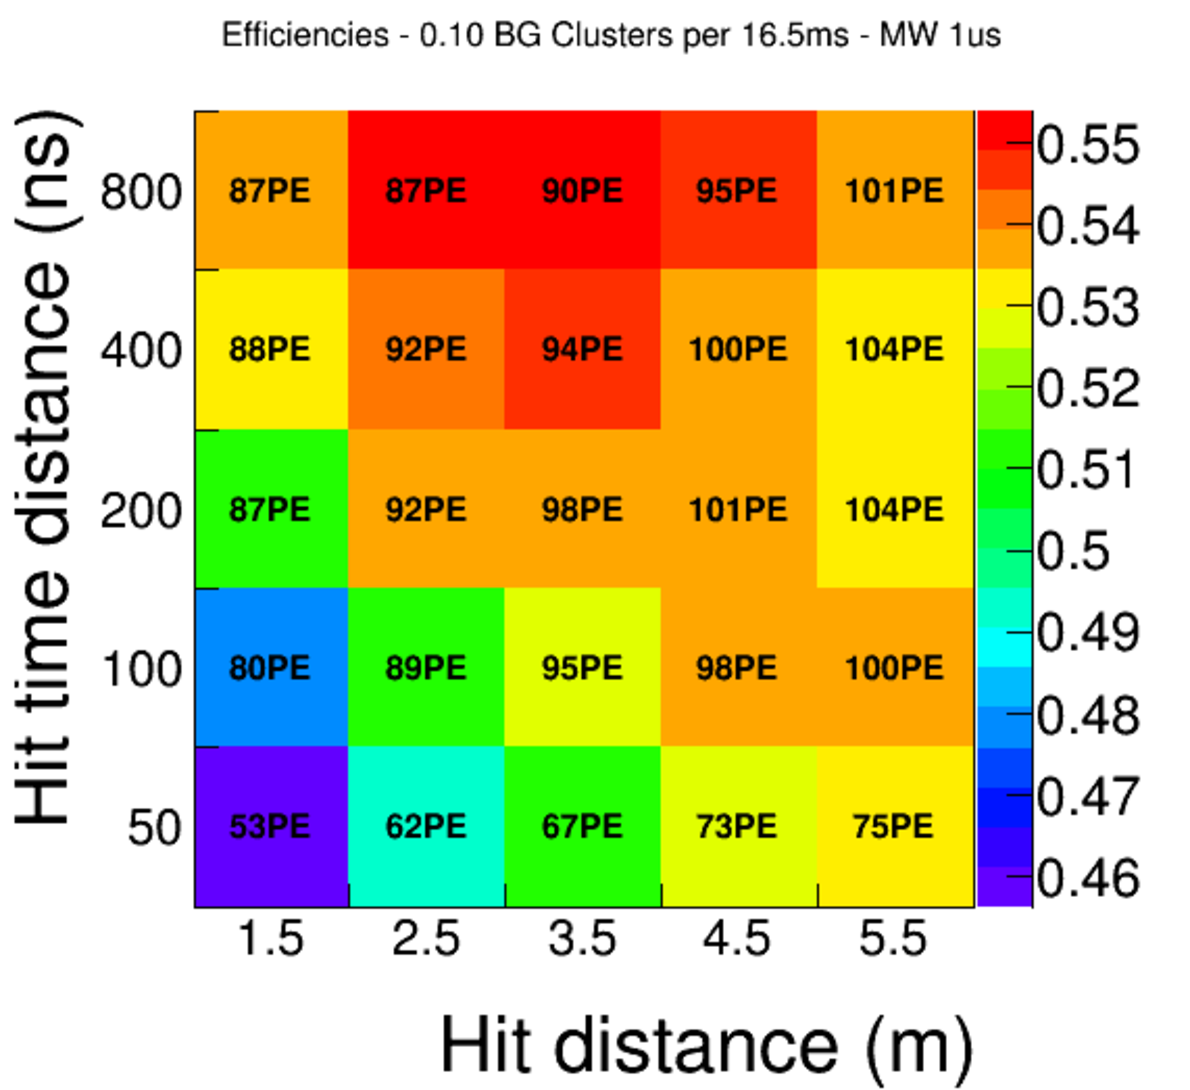
\includegraphics[width=0.5\textwidth]{graphics/dppd_ndk_optimization.pdf}
\end{dunefigure}

Figure~\ref{fig:dppd_ndk_optimization} illustrates how the \dword{ndk} signal efficiency, purity, and efficiency$\times$purity averaged over the entire \dword{tpc} active volume vary as a function of the maximum \twod distance between the $t_0$ candidate cluster reconstructed position and the \dword{ndk} vertex actual position in the plane perpendicular to drift. A maximum distance of \SI{1.5}{\m} optimizes the product of efficiency$\times$purity. 

Figure~\ref{fig:dppd_ndk_efficiency} shows how the \dword{ndk} $t_0$ reconstruction efficiency and purity vary as a function of the nucleon decay vertex distance from the cathode plane for the optimal cluster reconstruction parameters described above. Two configurations are compared: the proposed baseline design with half foils, and a design with no foils along the \dword{fc}. For the baseline design, both the efficiency and purity remain $>90\%$ throughout a \dword{tpc} fiducial volume excluding the upper \SI{70}{cm} of the \dword{tpc} active volume, satisfying the detector requirements laid out in Section~\ref{subsec:dp-pds-requirements_requirements}. From Figure~\ref{fig:dppd_fd_light_yield_comparisons}, a light yield of \SI{1}{PE/\MeV} is expected at the anode plane in the half-foil simulation. Because of this, the \dword{pds} minimum light yield required at the anode position is also \SI{1}{PE/\MeV} (see Table~\ref{tab:specs:DP-PDS}). 

On the other hand, for the no foil configuration, both efficiency and purity drop rapidly at large distances from the cathode. This is due to the marked reduction in the detected \dword{ndk} light yield as the energy deposition occurs at increasingly larger distances from the cathode, see Figure~\ref{fig:dppd_fd_light_yield_comparisons}. In this case, the efficiency (purity) remains $>90\%$ only for distances up to \SI{10}{\m} (\SI{7}{\m}) from the cathode (Figure~\ref{fig:dppd_ndk_efficiency}). This large improvement in efficiently and accurately reconstructing event $t_0$ information for \dword{ndk} events is the main, but not sole, motivation to introduce reflector/\dword{wls} foils along the \dword{fc} walls in the baseline design.

\begin{dunefigure}[Nucleon decay $t_0$ reconstruction efficiency and purity.]{fig:dppd_ndk_efficiency}
     {Nucleon decay $t_0$ reconstruction efficiency (left panel) and purity (right), defined in text, as a function of decay vertex distance from the cathode. Two \dword{pds} designs are compared: no foils and half foils (baseline). The anode plane is at a drift position of \SI{+600}{\cm}, the cathode plane at a drift position of \SI{-600}{\cm},  and \dword{pmt} plane is at a drift position of \SI{-700}{\cm}.}
    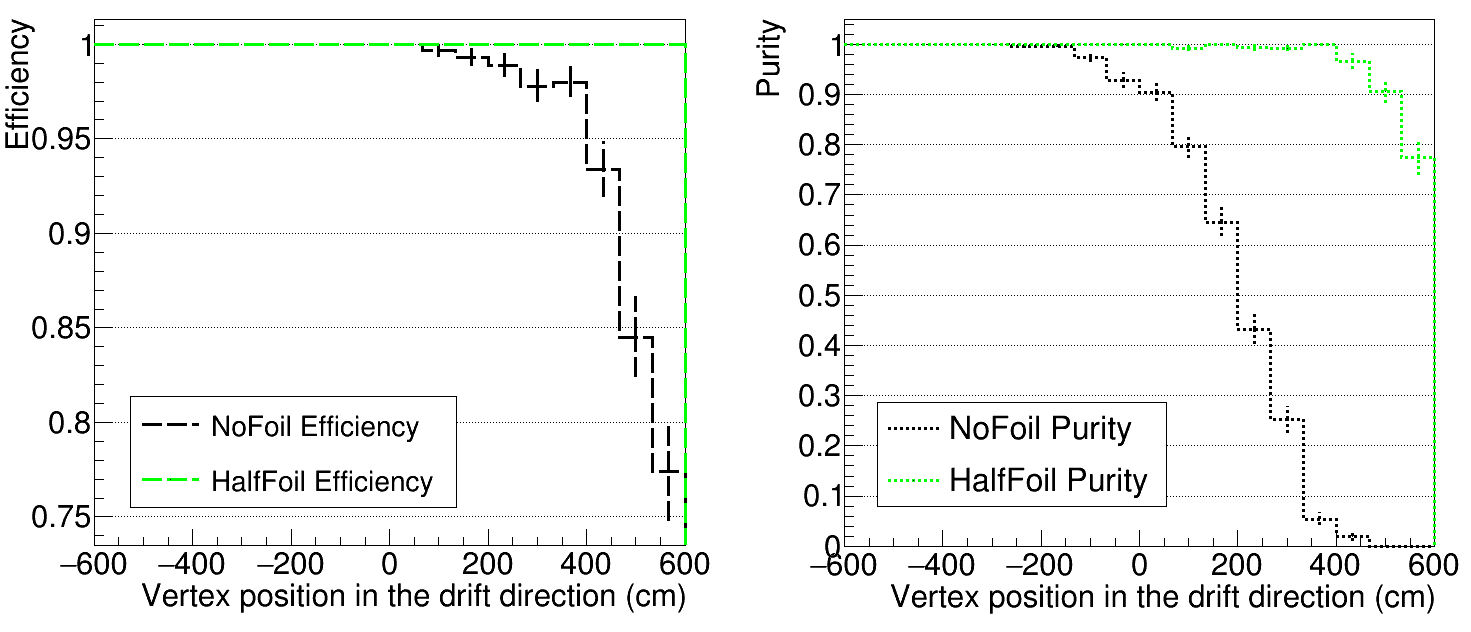
\includegraphics[width=0.90\textwidth]{graphics/dppd_ndk_efficiency.png}
    \end{dunefigure}

%%%%%%%%%%%%%%%%%%%%%%%%%%%%%%%%%%%%%%%%%%%%%%%%%%%%%%%%%%%%%%%%%%%%

\subsection{Supernova Burst Triggering}
\label{subsec:dp-pds-performance_trigger}

We have also studied how well the \dword{dp} \dword{pds} triggers on an \dword{snb} occurring in our galactic neighborhood. As described in Section~\ref{sec:dp-pds-requirements}, this is one of the primary goals of the \dword{pds}. To this end, \dword{snb} \nue \dword{cc} interactions have been generated with \dword{marley}~\cite{marley} in our baseline \dword{pds} design. In \dword{dune}, a real-time algorithm should provide trigger primitives by searching for \dword{pmt} hits and optical clusters, where the latter combine several hits together based on their time and spatial information. Compared to the \dword{ndk} case, the reconstructed optical signals are much weaker because the typical deposited energies per \dword{snb} neutrino interaction are approximately \SI{20}{\MeV}. The online clustering process is similar to the offline cluster reconstruction discussed in Section~\ref{subsec:dp-pds-performance_t0}, albeit with some differences related to the lack of trigger information and detailed event reconstruction at this stage:
%
\begin{itemize}
\item Real-time optical clusters must have a minimum hit multiplicity to suppress clusters induced by radiological activity or \dword{pmt} dark counts. The higher the hit multiplicity, the lower the background cluster rate.
\item \dword{pds} spatial information is only used to group hits into separate clusters,  not to match \dword{pds} clusters with \dword{tpc} tracks in the plane perpendicular to the drift, as in Section~\ref{subsec:dp-pds-performance_t0}.
\item Real-time optical clusters must be continuously reconstructed, while in Section~\ref{subsec:dp-pds-performance_t0}, only the \SI{7.5}{\milli\s} period preceding a charge-based trigger signal, corresponding to the maximum drift time, is considered.
\end{itemize}
%
The optimal real-time cluster reconstruction parameters yield a \SI{0.05}{\Hz} radiological background cluster rate for an \dword{snb} \nue \dword{cc} signal cluster efficiency of \SI{11.8}{\%}. Once the optimal cluster parameters are found, the computation of the \dword{pds}-based \dword{snb} trigger efficiency as a function of \dword{snb} distance is performed as follows:

\begin{itemize}
\item First, the minimum number of reconstructed clusters required in a \SI{2}{\s} time window  to issue a trigger is found\footnote{A \SI{2}{\s} time window was found to be optimal and is assumed throughout this section.}. The minimum cluster multiplicity is set by the requirement of no more than one fake trigger per month (see Section~\ref{sec:dp-pds-requirements}) and by the radiological background cluster rate. The higher the background cluster rate, the higher the minimum cluster multiplicity must be to meet the $<$\num{1}/month fake trigger rate requirement. For a background cluster rate of \SI{0.05}{\Hz}, a minimum cluster multiplicity of $\ge$\num{3} per \SI{2}{\s} time window is required for a $<$\num{1}/month fake trigger rate.
%
\item Second, the \dword{snb} triggering efficiency as a function of the number of \dword{snb} interactions is computed. For a \SI{11.8}{\%} average efficiency of reconstructing single \dword{snb} \nue interactions with the \dword{pds}, and a minimum cluster multiplicity of three to issue a trigger, approximately \num{3}/\num{0.118}$\simeq$ \num{25} interactions must occur in the \dword{fd} module and within \SI{2}{\s} to obtain a non-negligible trigger efficiency. 
%
\item Third, and finally, the \dword{snb} triggering efficiency as a function of \dword{snb} distance is obtained. We use the theoretical assumptions shown in Figure~\ref{fig:dppd_snbassumptions} to extract the number of \dword{snb} neutrino interactions in a \SI{2}{\s} time window %and 
in one \dword{dpmod} as a function of \dword{snb} distance. The left panel of Figure~\ref{fig:dppd_snbassumptions} shows the time-integrated expected number of \dword{snb} neutrino interactions with greater than \SI{10}{MeV} neutrino energy as a function of distance, while the right panel in Figure~\ref{fig:dppd_snbassumptions} shows the assumed time profile of the burst during the first \SI{10}{\s}. Several hundred \dword{snb} neutrino interactions are expected in one \dword{dp} \dword{fd} module for a \SI{10}{\kilo\parsec} distant \dword{snb}\footnote{It is customary to evaluate the performance of \dword{snb} detectors for a \dword{snb} distance of \SI{10}{\kilo\parsec}, as this is approximately the distance to the Galactic Center.}, and about half of them are expected within the first \SI{2}{\s}. Given our earlier estimate that about \num{25} interactions should be sufficient for a non-negligible trigger efficiency, clearly the \dword{pds} should provide high \dword{snb} trigger efficiency for an \dword{snb} at a \SI{10}{\kilo\parsec} distance. Given the large uncertainty in the number of interactions expected at a certain \dword{snb} distance introduced by \dword{snb} models, we present our trigger efficiency results below not only as a function of \dword{snb} distance, but also as a function of number of \dword{snb} interactions. 
\end{itemize}

\begin{dunefigure}[SNB triggering assumptions]{fig:dppd_snbassumptions}
     {Left panel: expected number of \dword{snb} \nue \dword{cc} interactions in one \dpactivelarmass active mass \dword{dpmod} as a function of \dword{snb} distance. The different green lines indicate different \dword{snb} models. Right panel: expected time profile of the \dword{snb}.}
    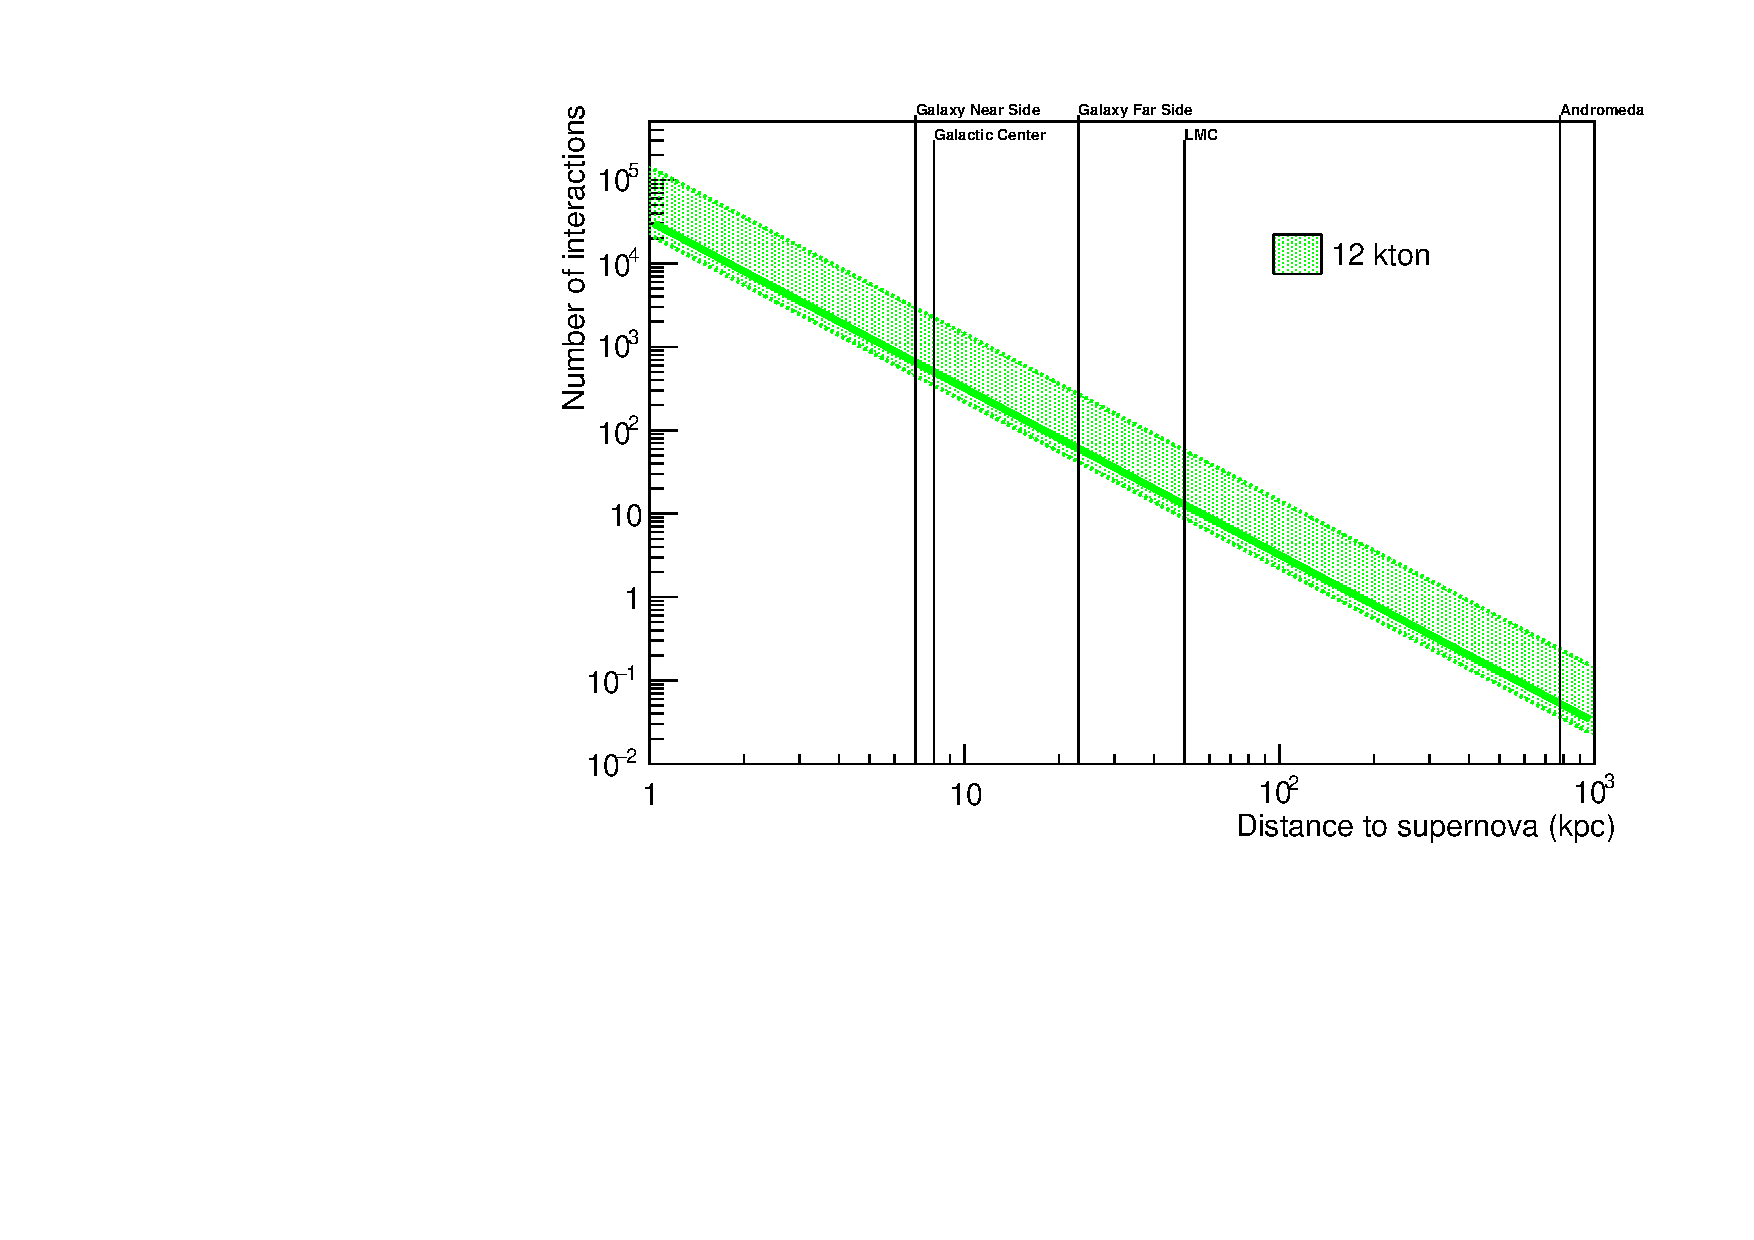
\includegraphics[width=0.49\textwidth]{graphics/dppd_events_vs_sndistance.pdf} \hfill
    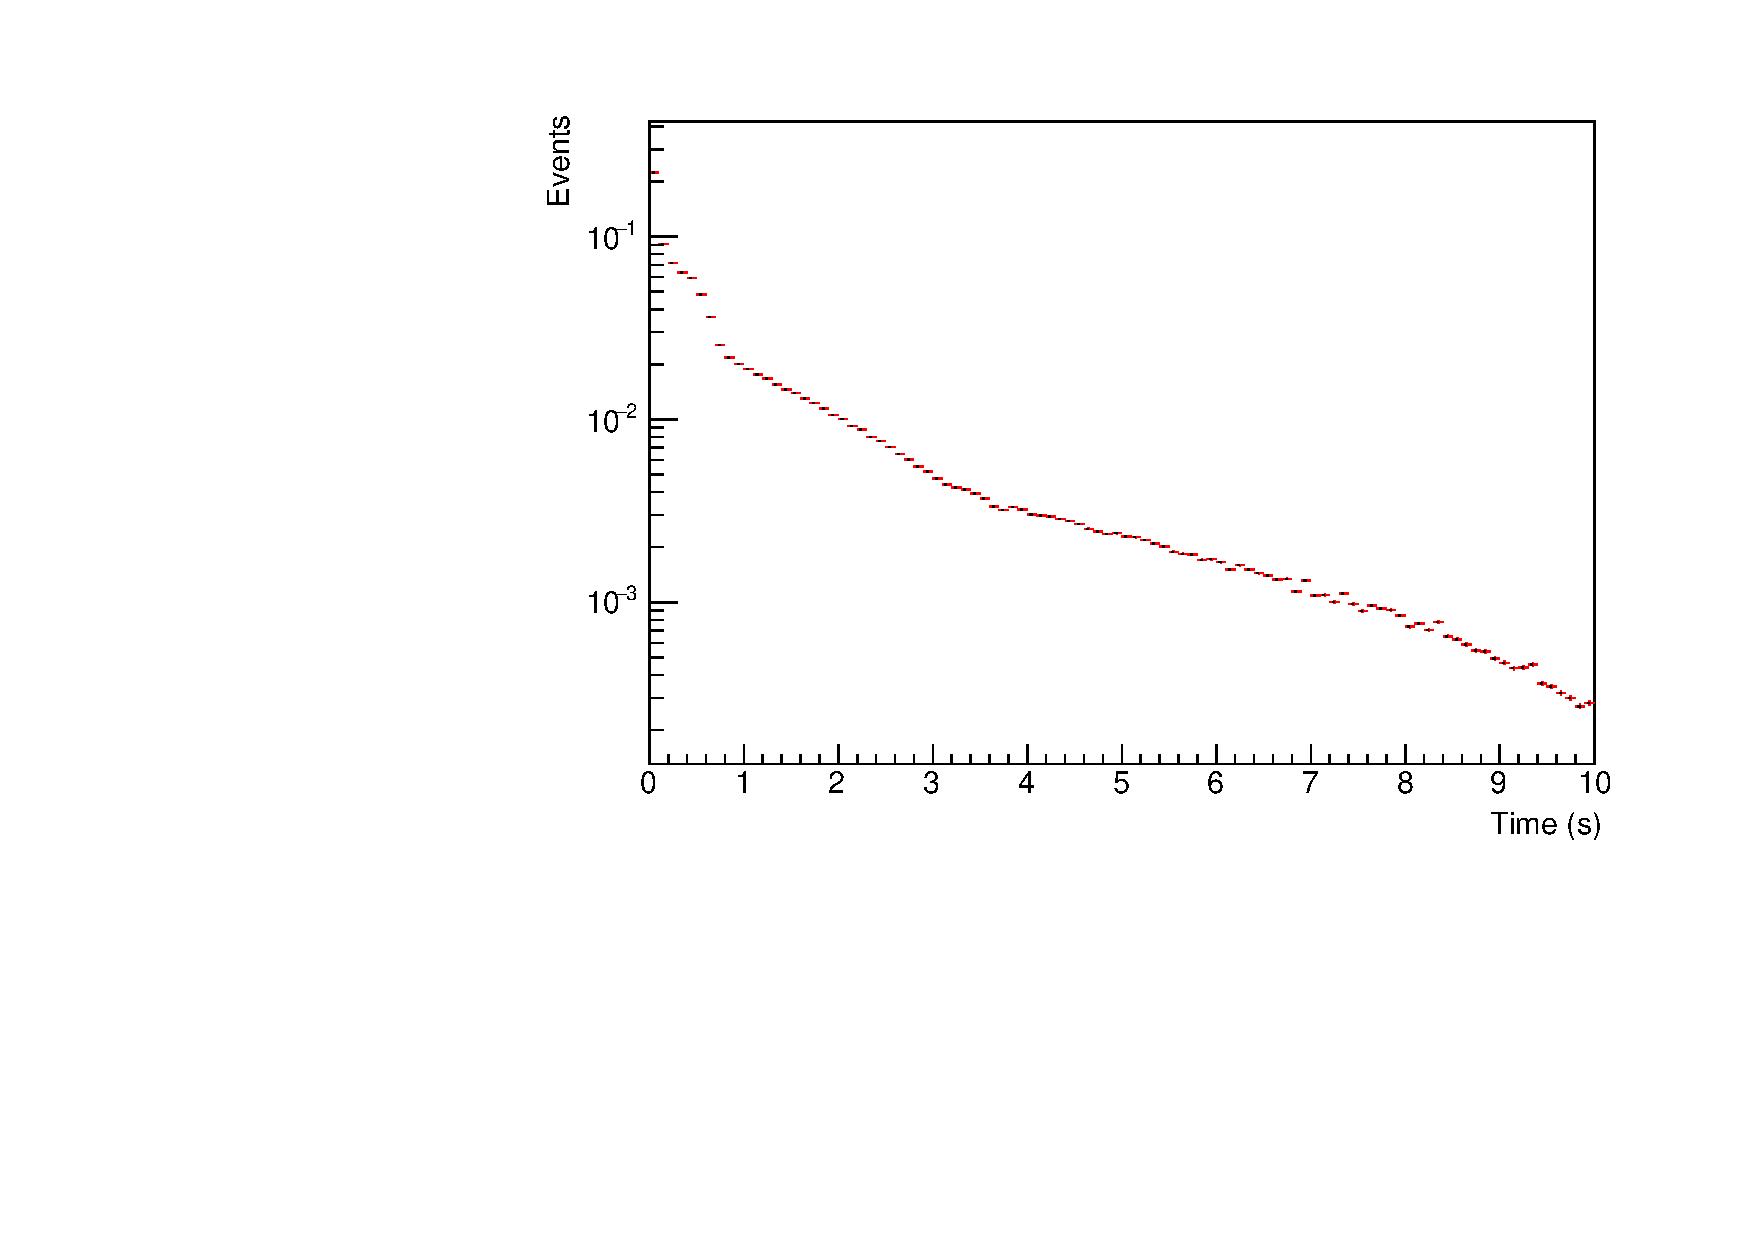
\includegraphics[width=0.49\textwidth]{graphics/dppd_sntime_profile.pdf} 
    \end{dunefigure}

Figure~\ref{fig:dppd_snbefficiency} shows the \dword{snb} triggering efficiency for the half-foil baseline \dword{pds} design, both as a function of the number of \dword{snb} interactions in the active volume and as a function of \dword{snb} distance for a standard \dword{snb} model. A trigger efficiency in excess of \num{90}\% is obtained for \num{60} \dword{snb} interactions, as required in Section~\ref{sec:dp-pds-requirements}, in order to have a highly efficient trigger for \dwords{snb} occurring anywhere in the Milky Way. For the standard \dword{snb} model shown, this efficiency is maintained up to \dword{snb} distances of approximately \SI{24}{\kilo\parsec}. At the \SI{20}{\kilo\parsec} distance of the galaxy edge, about \num{80} \dword{snb} interactions in the \dpactivelarmass active mass are expected for this particular \dword{snb} model. The \dword{snb} triggering requirement motivates the $>\,$\SI{5}{\dwords{pe}/\MeV} average light yield specification in Table~\ref{tab:specs:DP-PDS}, since a similar light yield is expected in our baseline design.

Figure~\ref{fig:dppd_snbefficiency} also shows how the \dword{snb} trigger efficiency of the baseline configuration compares with alternative choices, namely no foils and full foils. Our minimum \dword{snb} trigger efficiency requirement of \num{90}\% for \num{60} \dword{snb} interactions or more would not be reached for the no-foil configuration. On the other hand, the results improve noticeably with full foil coverage. 

\begin{dunefigure}[\dshort{snb} triggering efficiency for different \dshort{wls} foil configurations]{fig:dppd_snbefficiency}
     {\dword{snb} triggering efficiency as a function of \dword{snb} interactions in the active volume (left panel) and as a function of \dword{snb} distance (right panel) for three different \dword{wls} foil configurations.}
     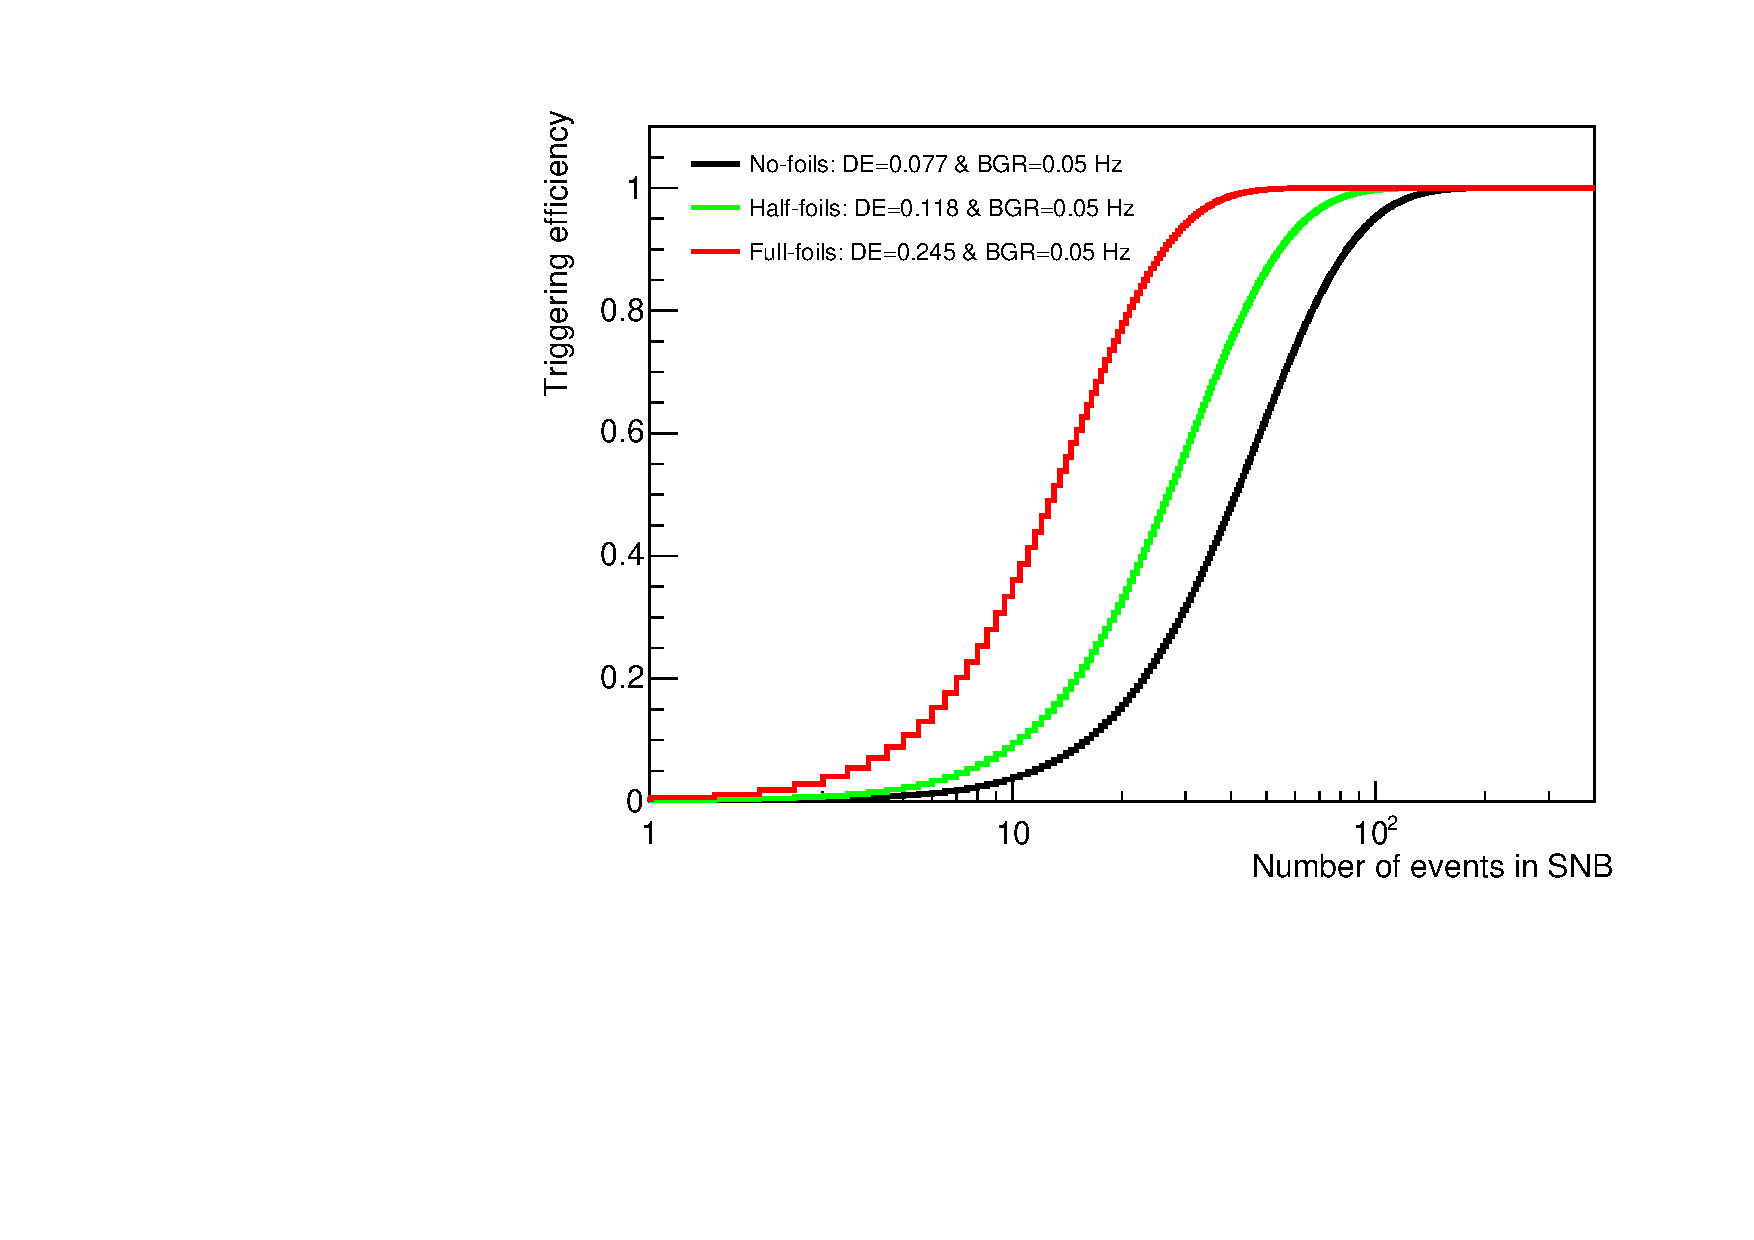
\includegraphics[width=0.49\textwidth]{graphics/dppd_snbefficiency_vs_snevents.pdf} \hfill
    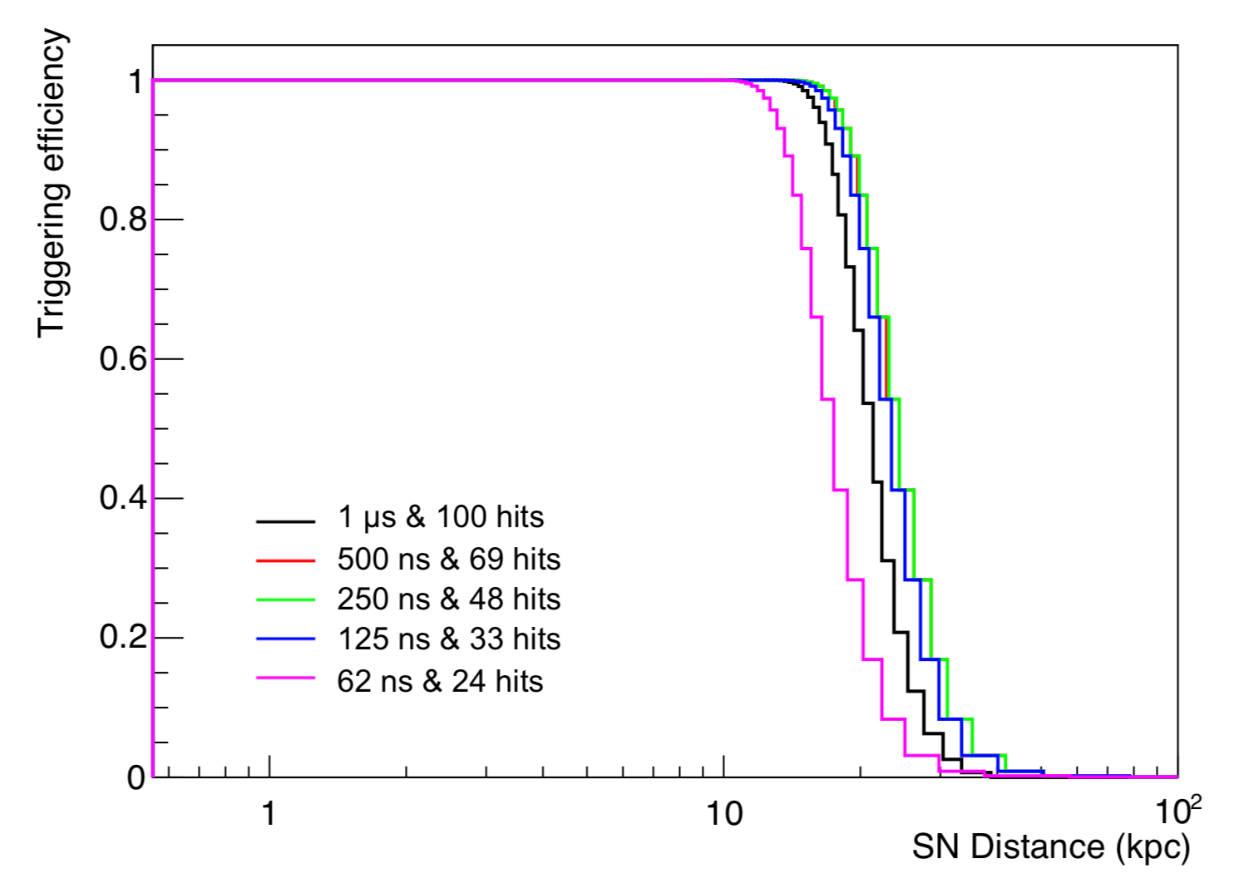
\includegraphics[width=0.49\textwidth]{graphics/dppd_snbefficiency_vs_sndistance.pdf}
    \end{dunefigure}

%%%%%%%%%%%%%%%%%%%%%%%%%%%%%%%%%%%%%%%%%%%%%%%%%%%%%%%%%%%%%%%%%%%%

\subsection{Event Energy Reconstruction}
\label{subsec:dp-pds-performance_calorimetry}

In addition to timing and triggering information, the \dword{pds} can also provide event energy information via the intensity of the reconstructed optical flashes. We focus in this section on beam neutrino interactions generated via the \dword{genie} event generator \cite{Andreopoulos:2009rq}, as described in Section~\ref{subsec:dp-pds-requirements_requirements}.

A first requirement for a competitive energy reconstruction performance with the \dword{pds} is that the \dword{pds} and associated readout electronics keep optical hit saturation effects to a manageable level. Figure~\ref{fig:dppd_saturation} shows the expected average hit charge and average hit amplitude as a function of drift position of the neutrino interaction vertex for \SI{3}{\GeV} beam \nue \dword{cc} interactions. For each event, the average is computed by considering hit \dword{pds} channels only, that is, \dwords{pmt} detecting a charge of at least \SI{1}{\dword{pe}}. The average hit charge per event is approximately \SIrange{50}{300}{} for \SI{3}{\GeV} beam \nue \dword{cc} interactions throughout the \dword{tpc} active volume. The average charge is expressed in \dwords{pe}, with the average amplitude in \dwords{pe} per \SI{4}{\nano\s} time bin. This time bin width is comparable with the \SI{6}{\nano\s} timescale characteristic of the prompt scintillation light in \dword{lar}. For events near the cathode plane, about \SI{300}{\dwords{pe}} per hit channel are detected, corresponding to a maximum amplitude over \SI{4}{\nano\s} of about \SI{50}{\dwords{pe}}. The factor of six difference between average charge and average amplitude is due to the fact that only \SI{23}{\%} of the scintillation light is prompt and (to a smaller extent) due to additional time-smearing introduced by light propagation to the same \dword{pmt} from different \dword{lar} voxels containing energy deposits. From these plots, we conclude that the \dword{pds} signal readout should withstand signal amplitudes of at least \SI{100}{\dwords{pe}} over \SI{6}{\nano\s} to mitigate saturation effects (see Table~\ref{tab:specs:DP-PDS}).

\begin{dunefigure}[Average charge and amplitude per hit channel in beam neutrino interactions]{fig:dppd_saturation}
{Expected average hit charge (left panel, in \dwords{pe}) and average hit amplitude (right panel, in \dwords{pe} per \SI{4}{\nano\s} time bin) as a function of event drift position for \SI{3}{\GeV} beam \nue \dword{cc} interactions. The scatter plots  contain one entry per event, and the average is for hit \dword{pds} channels only.}
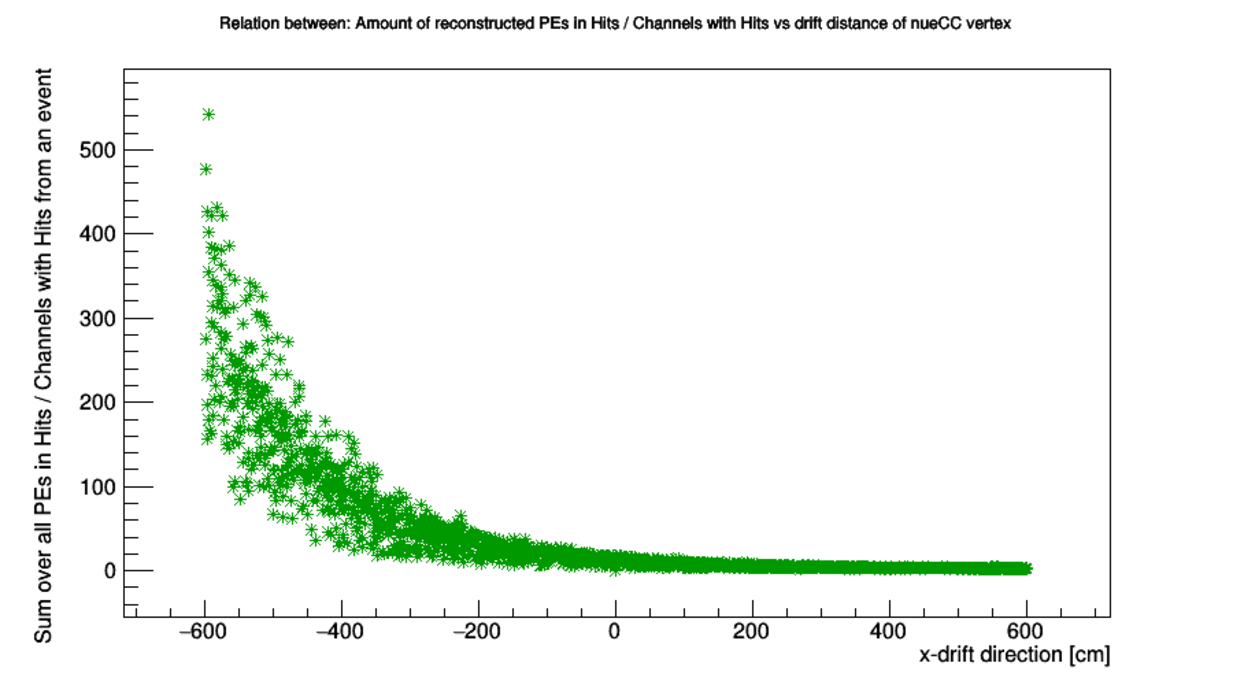
\includegraphics[trim={0cm 0cm 0cm 1.cm}, clip, width=0.49\textwidth]{graphics/dppd_avg_charge_per_channel.pdf} \hfill
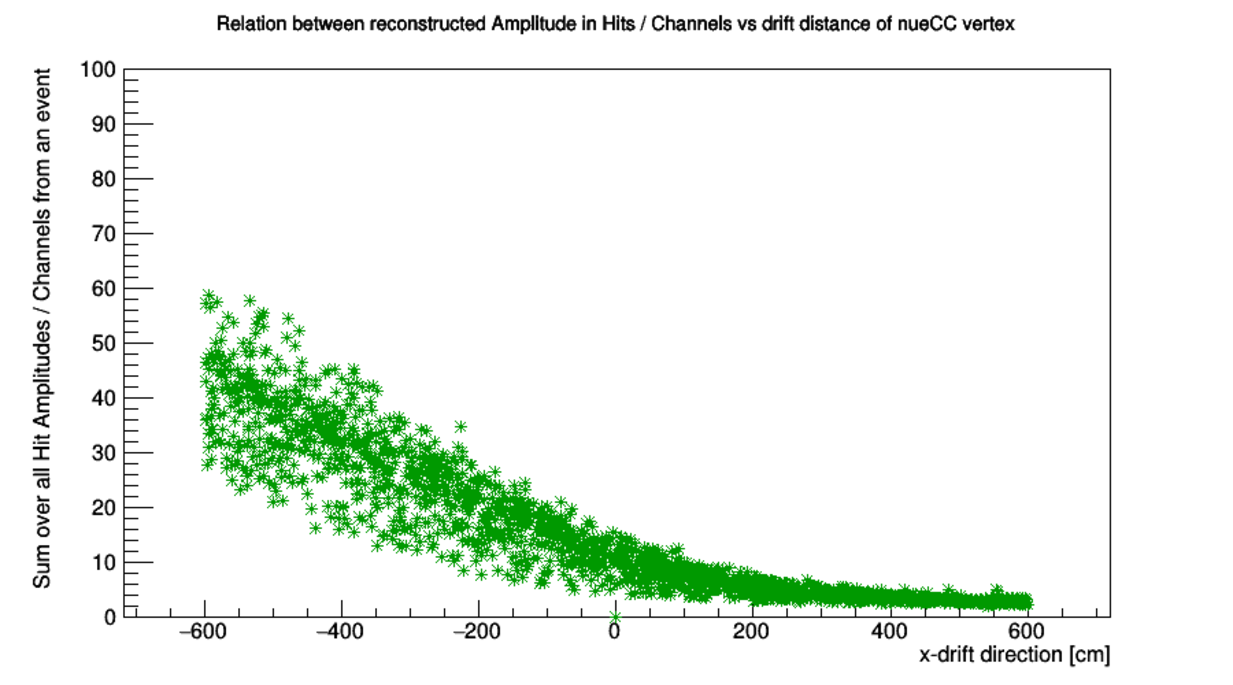
\includegraphics[trim={0cm 0cm 0cm 1.cm}, clip, width=0.49\textwidth]{graphics/dppd_avg_amplitude_per_channel.pdf}
\end{dunefigure}

The neutrino energy using \dword{pds} information is reconstructed as follows:
\begin{itemize}
\item Since the energy is proportional to the total charge (in \dwords{pe}) of all \dword{pmt} hits reconstructed in the event, we consider only hits within \SI{10}{\micro\second} of the neutrino interaction time in order to reduce biases due to \dword{pmt} dark counts.
%
\item We then estimate the number of scintillation photons produced in the \dword{lar} by dividing the total charge by an average \dword{pds} visibility (in detected \dwords{pe} per produced scintillation photon). The average visibility strongly depends  on spatial location, but % and 
also on event topology. For this correction, we use the same light maps used to simulate the light of our baseline detector design. The average visibility is computed using an extended track model, assuming that the \dword{tpc} information provides the spatial pattern of energy deposits within the detector. 
%
\item The reconstructed number of scintillation photons is then converted into energy by dividing by a scintillation light yield of \SI{2.4e4}{photons/MeV}.
%
\item Finally, we apply a simple, energy-independent, multiplicative factor of 1.26  to the reconstructed energy to account for energy reconstruction biases. This multiplicative factor was found empirically, using simulated \SI{3}{\GeV} beam \nue \dword{cc} interactions. The bias is mainly due to scintillation-light quenching from Birk's effect, which suppresses %resulting in a suppression in 
the amount of visible energy (in the form of scintillation light) compared to the energy deposited in the \dword{lar}. While Birk's formula depends in general on particle type and $dE/dx$ along the tracks, the average light quenching per neutrino interaction is independent of spatial location, and to a first approximation, %is also independent 
of neutrino energy. 
\end{itemize}

The left panel of Figure~\ref{fig:dppd_beam_calorimetry_3GeV} shows the event energy reconstructed in this way  as a function of event deposited energy, for a sample of \SI{3}{\GeV} \nue \dword{cc} interactions occurring in the \dword{lar} fiducial volume. The plot shows a high degree of correlation between reconstructed and deposited energy, as desired. The right panel of Figure~\ref{fig:dppd_beam_calorimetry_3GeV} shows the deposited energy resolution for the same \SI{3}{\GeV} interactions, resulting in a Gaussian resolution function of about \num{7}\% width. However, as also illustrated in the left panel of Figure~\ref{fig:dppd_beam_calorimetry_3GeV}, the deposited energy shows a significant downward bias and large event-by-event fluctuations compared to the fixed \SI{3}{GeV} neutrino energy of the simulated event sample. The bias and \dword{rms} spread are significant, of order \num{10}\% each. They are due to energy lost in nuclear breakup and in neutral particles (gamma rays, neutrons, and secondary neutrinos from pion and muon decay) escaping the detector, see for example \cite{Friedland:2018vry}. In other words, the bias and spread in the deposited energy distribution shows how well an ideal detector could reconstruct the neutrino event energy in a model-independent way.

\begin{dunefigure}[Deposited energy and PDS-reconstructed energy for \SI{3}{GeV} interactions]{fig:dppd_beam_calorimetry_3GeV}
{Energy reconstruction for \SI{3}{GeV} \nue \dword{cc} interactions in the \lar fiducial volume. Left panel: \dword{pds}-reconstructed energy versus deposited energy. Right panel: pull of reconstructed minus deposited energy, divided by deposited energy, yielding a \num{7}\% deposited energy resolution.}
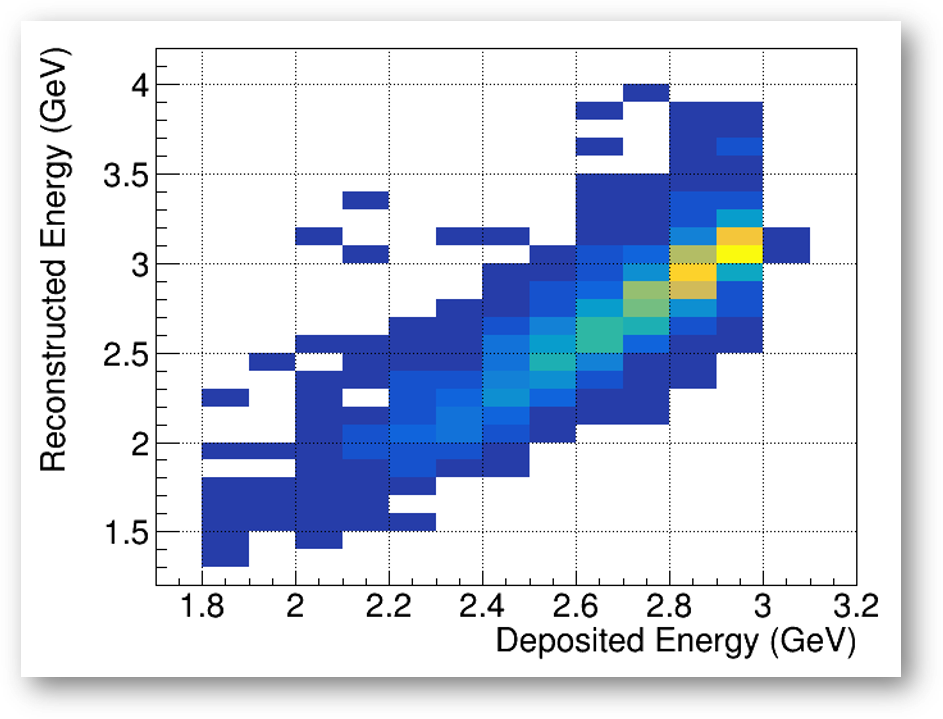
\includegraphics[width=0.49\textwidth]{graphics/dppd_ereco_vs_edep_nuecc_3gev.png} \hfill
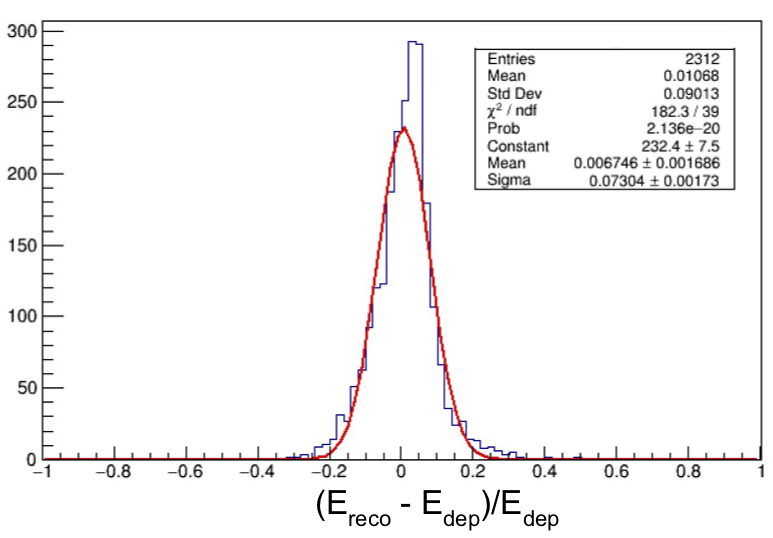
\includegraphics[width=0.49\textwidth]{graphics/dppd_edep_resolution_nuecc_3gev.png}
\end{dunefigure}
\fixme{``pull'' of reconstructed minus deposited energy?}

Figure~\ref{fig:dppd_energyresolutions_nuecc} shows the expected resolutions in deposited  energy and in neutrino  energy using the \dword{pds}, for beam \nue \dword{cc} interactions in the \SIrange{1}{8}{GeV} range and in the \dword{lar} fiducial volume. Deposited energy resolutions are expected to be better than \num{10}\% for all beam neutrino energies of interest to DUNE, while the neutrino energy resolution is expected to be of order \num{15}\%. This is a very promising result, in principle, competitive with neutrino energy resolutions achievable with the \dword{tpc}.

\begin{dunefigure}[Energy resolutions for few-GeV beam neutrino interactions using the \dshort{pds}.]{fig:dppd_energyresolutions_nuecc}
{Resolution of how well the deposited energy (red) and the neutrino energy (blue) can be reconstructed using the \dword{pds}, as a function of neutrino energy for \nue \dword{cc} interactions in the \lar fiducial volume.}
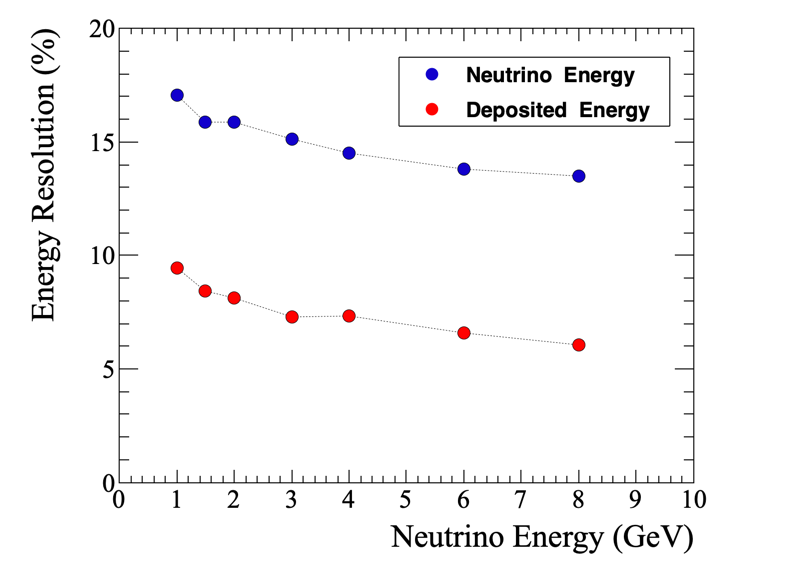
\includegraphics[width=0.60\textwidth]{graphics/dppd_energyresolutions_nuecc.png}
\end{dunefigure}

\section{Quality Control and Quality Assurance}
\label{sec:dp-pds-quality}

The \dword{qa} and \dword{qc} procedures for the \dual \dword{pds} are based on our experience with the \dword{pddp}. The \dwords{pmt} of the \dual \dword{pds} will go through a series of performance and functionality tests at various locations until commissioning. The mechanical assembly of the \dwords{pmt} will go through mechanical tests, the high voltage cables will be tested for continuity and resistance, the high voltage/signal splitters will be tested for electronics integrity, and the calibration fibers will be tested for high quality transmission. Below  are the details of the quality assurance and control procedures.

\subsection{Quality Control During Production and Assembly}

The \dword{qc} performed at the different institutions includes reception of the \dwords{pmt} from the manufacturer and execution of the \dword{qc} tests to accept or return the \dwords{pmt} according to the acceptance and rejection criteria; \dword{qc} of the construction of the base boards, support structures, cables, \dword{hv}/signal splitters and light calibration units. The testing will involve the mechanical tests of the assembly, performance tests of the \dwords{pmt} and electronics both at room temperature and when necessary, at cryogenic temperatures. The institutes that perform these activities are hereby referred to as production and assembly sites.

\begin{itemize}
\item The \dwords{pmt} will be visually inspected as they are received from the manufacturer.

\item 
%The baseboards will be tested for electronics integrity as they are produced, before they are connected to the \dwords{pmt}. Once they are connected, mechanical integrity will be tested. 
The \dword{pmt} support structure design is already validated by immersing its mounted \dword{pmt} in cryogenic temperatures and at an over-pressure equivalent to a depth of \SI{12}{m} in \lar{}. Design validation tests are carried out to confirm that the \dword{pmt} base design fulfills the specifications at room and cryogenic temperatures. A cable with SHV connector is soldered to each \dword{pmt} base to facilitate the different base and \dword{pmt} tests and the final \dword{pmt} connection during the installation. The \dword{pmt} bases are labeled (on the cable) in order to keep track of them. After production of the \dword{pmt} base boards they are individually tested before connecting to the \dwords{pmt} to verify that components are correctly mounted. Later they are cleaned and tested at maximum voltage in an argon gas environment to confirm that there are no sparks. After mounting the bases on the \dwords{pmt}, they are tested again %in argon gas 
at maximum voltage to confirm that there are no sparks due to bad soldering.

\item All the light readout units (\dword{pmt} + base + support) will be tested and characterized in liquid nitrogen in order to check their performance at cryogenic temperature and to obtain a database with the most important parameters for each \dword{pmt} (gain versus voltage, dark counts, etc.). The \dword{pmt} base number attached to each \dword{pmt} will also be included in the database.

\item The wrapping materials and techniques are studied with one fully assembled light readout unit. The handling, transportation and installation scenarios are carefully studied and the transportation box design is validated. The transport box and \dword{pmt} wrapping must  ensure complete darkness.

\item The light output of the \dwords{led} and the fibers' light transmission from the light calibration system will be measured with a power meter.

\item The high voltage cables will be tested for continuity and for their resistance.

\item The high voltage/signal splitters will be tested for electronics integrity followed by their performance with a reference \dword{pmt}.

\end{itemize}

\subsection{Quality Control at the Integration and Testing Facility}

The \dwords{pmt} will be transported to the \dword{itf}, which is planned to be constructed in South Dakota, in the proximity of the experiment site. As the \dword{pmt} boxes are received, they will be visually inspected to validate safe transportation. The \dword{tpb} coating of the \dword{pmt} windows will be performed at the \dword{itf}. The \dword{pmt} windows will be cleaned prior to the coating process. The \dword{qc} of the cleaning will be based on experience in a qualitative manner. The \dwords{pmt} will then be placed in the evaporator and the coating operations will be performed. The first few samples will undergo microscopic examination and surface uniformity tests, and the coating procedure will be validated. The production \dwords{pmt} will be randomly sampled for basic coating \dword{qa}.

Once the coating is finished, the \dwords{pmt} will be placed in the special underground transport assembly which will be placed inside the original transportation boxes. The \dwords{pmt} will not be placed in the carton boxes. They will have protective covers over the windows. Before being placed in the transportation assembly, the \dwords{pmt} will undergo functionality tests individually. Once all the \dwords{pmt} in a box are validated, the box will be closed and transported to the underground hall.

The \dword{itf} is also the primary reception point for the other \dword{dp} \dword{pds} equipment including the cables, fibers, light calibration systems and \dword{hv}/signal splitters. These boxes will be inspected for validating safe transportation. Unless there is a sign of obvious damage to the transportation boxes, no \dword{qc} inspection will be performed on the individual items. If potential damage is identified, the boxes will be opened and visual/functional \dword{qc} tests will be performed. In case the damaged items can be repaired, this operation will be performed at the \dword{itf}. In case the damage is not repairable, the items will be returned to the manufacturer or the production/assembly sites.

\subsection{Quality Control at the Underground Areas}

After  transportation from the \dword{itf} to \surf, the \dwords{pmt} will be tested for proper functionality in a dedicated light-tight box in the clean room. During the installation, the \dword{pmt} database will be updated with the position of each \dword{pmt} (identified by its serial number and base number) in the \dword{detmodule}. After installation, the full connection from the \dword{fe} to the \dwords{pmt} will be checked. The \dword{fe} channel and splitter number connected to each \dword{pmt} will be included in the \dword{pmt} database.

The \dword{hv}/signal cables and the calibration fibers will be transported to the cryostat roof long before the \dwords{pmt} themselves. As they arrive, they will be checked for potential damage during transportation. These tests will include continuity test for the \dword{hv}/signal cables and qualitative transmission test for the calibration fibers.

The last step of \dword{qc} will be to test the entire system using the full readout chain (Section~\ref{subsec:dp-pds-commissioning}).

\section{Interfaces}
\label{sec:fddp-pds-interfaces}



\section{Installation, Integration, and Commissioning}
\label{sec:dp-pds-installation}

\subsection{Transport and Handling}

\dwords{pmt} will be transported on a standard EUR pallet that is \SI{1.2}{\m} $\times$ \SI{1}{\m}. Figure~\ref{fig:dppd_11_2} shows the largest capacity commercially available box. The box can hold \num{36} \dwords{pmt} in three levels of \num{4} $\times$ \num{3} arrays. Individual \dwords{pmt} will be placed in cartons with their bases, support structures, and short \dword{hv} cables soldered to the bases at the production/assembly sites. For shipping to \dword{ctsf}, \num{36} \dwords{pmt} will then be placed in the transport boxes.

\begin{dunefigure}[Example transportation box]{fig:dppd_11_2}
{An example transportation box to be used to transport items from remote sites to the \dword{ctsf} and from \dword{ctsf} to \surf.}
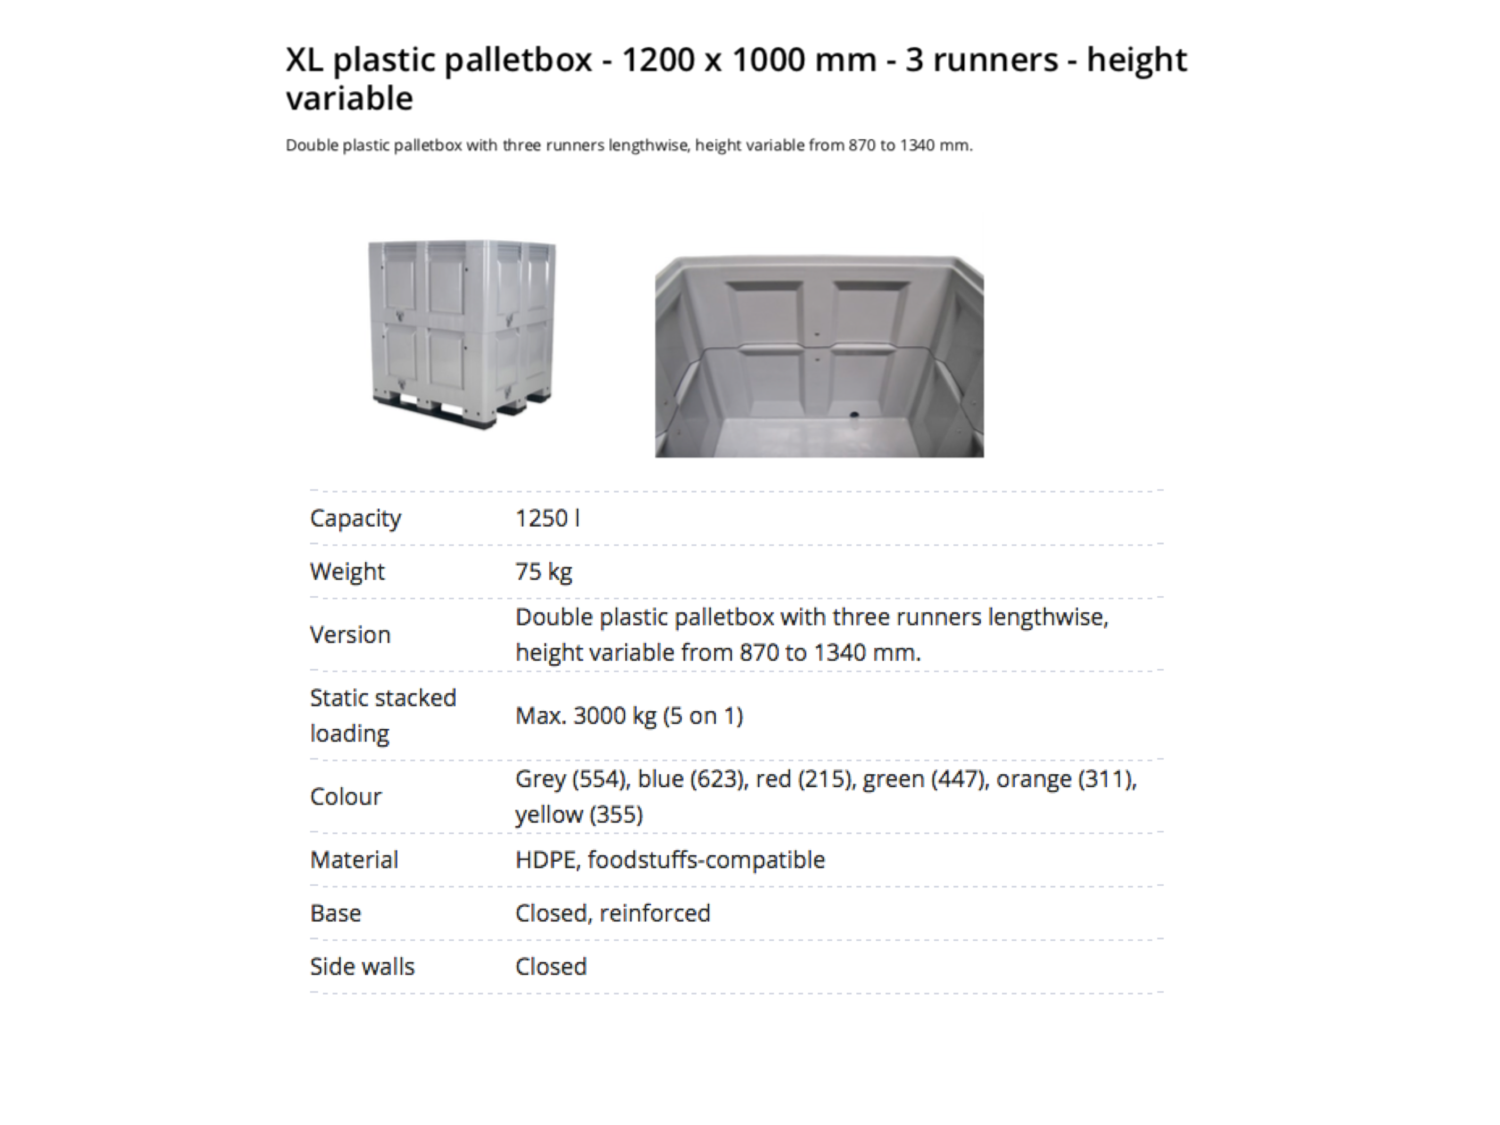
\includegraphics[width=0.5\textwidth]{dppd_11_2}
\end{dunefigure}

Following the \dword{ctsf} operations, the \dwords{pmt} will be placed in a custom structure in \num{4} $\times$ \num{3} arrays. The structure will be assembled with metal and plastic parts so the entire structure, together with the \dwords{pmt}, can be moved into the clean room underground. Three of these structures will be placed on top of each other inside the boxes with the crane. The individual cartons that held the \dwords{pmt} will be recycled at the \dword{ctsf}. The local movement of the transportation boxes in the \dword{ctsf} can be done with compact warehouse forklifts. The \dword{ctsf} will also be used as the storage area for the large \dword{pmt} transportation boxes before they are sent to \surf. The boxes will be stored in single-shelf racks to the right and left of the entrance to the work area (Figure~\ref{fig:dppd_11_3}). The first set of boxes will be placed on the floor and the second set will be on a shelf that is \SI{1.5}{\m} off the ground. This area can store the entire \dual \dword{pds} \dword{pmt} inventory of \dpnumpmtch \dwords{pmt} in \num{20} boxes. The \num{80} spare \dwords{pmt} can be placed in three boxes, which can be stored on the floor in the available space in the work area as the \dual \dword{pds} \dword{ctsf} operations are finished.

The large \dword{pds} boxes will be wrapped with plastic foil at the \dword{ctsf} that will be opened in \dwords{sas} underground. After removing the plastic wrapping, the transport boxes, with their entire contents, will be moved into the cleanroom. The \dword{pds} boxes can be moved around the underground areas with a pallet jack. Each \num{4} $\times$ \num{3} structure will be removed from the transportation box and moved inside the cleanroom by the crane. The structure will go in the dark box for functionality tests of the \num{12} \dwords{pmt}. The transportation boxes will be used for storage before installation. Empty boxes will be returned to \dword{ctsf}. At most, three \dword{pds} boxes will be in the cleanroom at a time.

The \num{4} $\times$ \num{3} structure will be moved by crane into the cryostat and placed on the cryostat floor at a location convenient to the active installation area. The \dwords{pmt} will then be installed one by one. 

%\subsection{Integration and Testing Facility Operations}
\subsection{Coating, Testing and Storage Facility Operations}
\label{subsec:dp-pds-itf}

The \dword{ctsf} will be \SI{10}{\m} $\times$ \SI{8}{\m} with a (\SI{12}{\ft}) ceiling equipped with a gantry crane. The facility will be used to apply the \dword{tpb} coating on the \dword{pmt} windows, for \dword{qc} of the \dwords{pmt}, and for storage and preparation for transport to \surf. If the option of installing individual ground grids on the \dword{pmt} support structures, which is under consideration by the \dual \dword{pds} and \dword{hv} consortia, is realized, this operation will also be performed at the \dword{ctsf}. The layout of the \dword{ctsf} is shown in Figure~\ref{fig:dppd_11_3}.

\begin{dunefigure}[The layout of the \dshort{ctsf}]{fig:dppd_11_3}
{The layout of the \dword{ctsf}.}
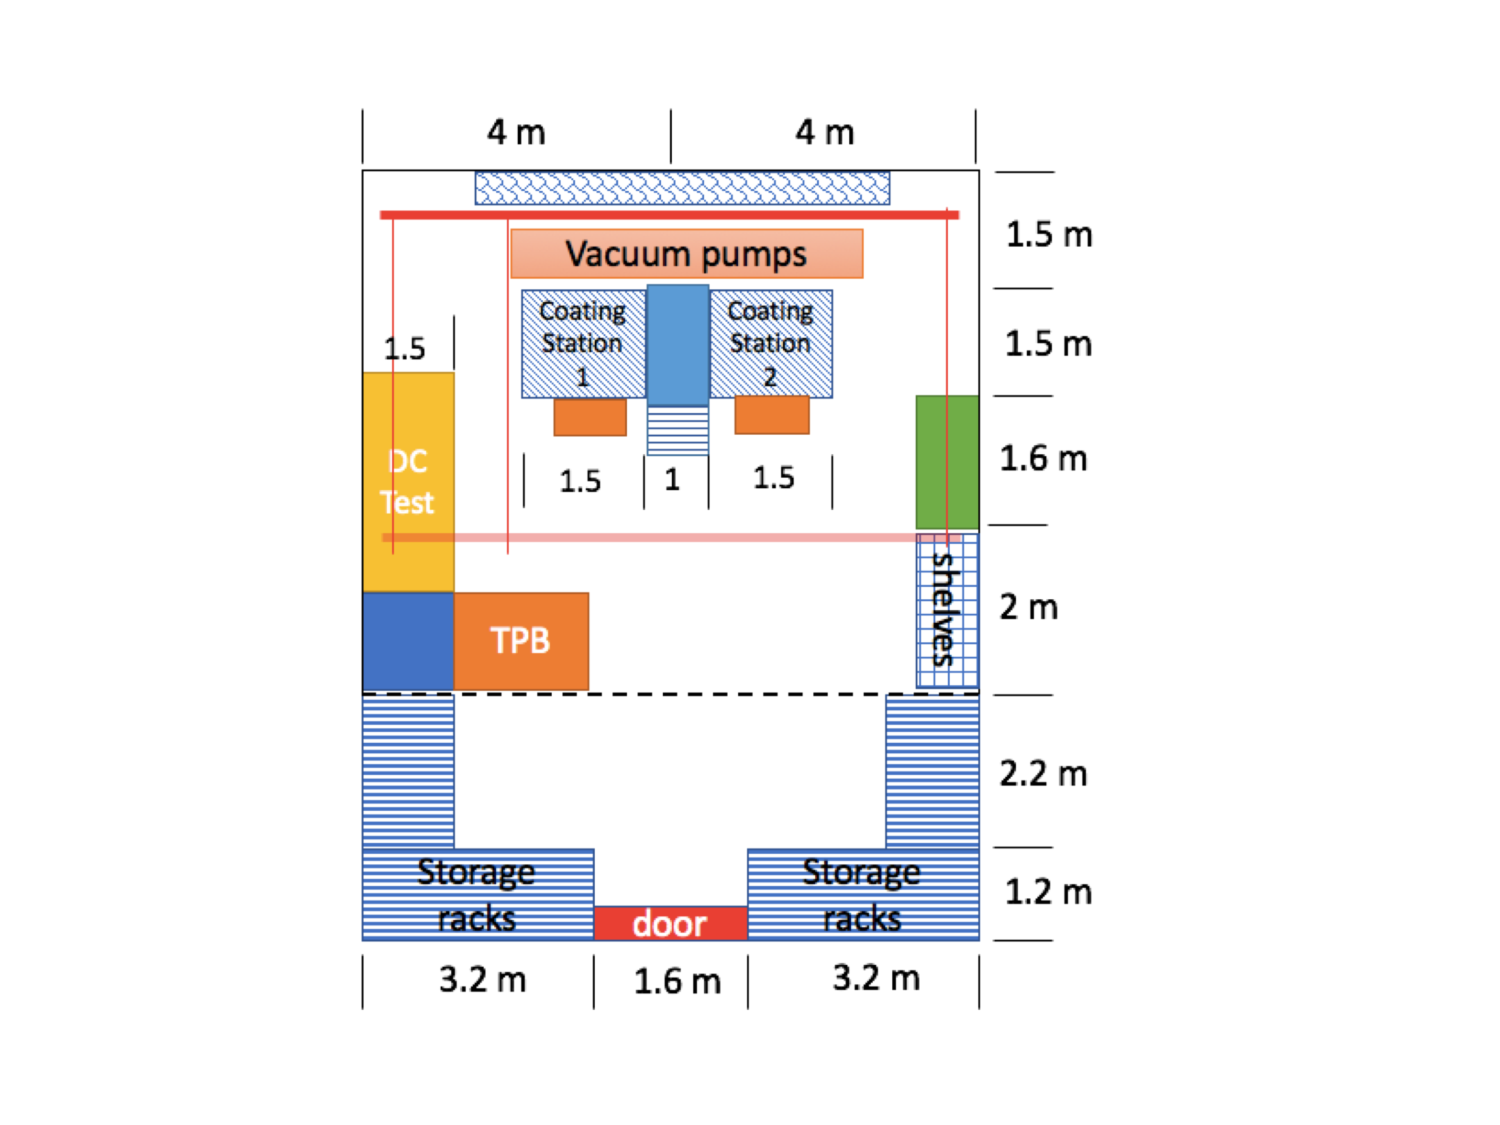
\includegraphics[width=0.4\textwidth]{dppd_11_3}
\end{dunefigure}

Two coating stations will be \SI{1.5}{\m} $\times$ \SI{1.5}{\m}. Figure ~\ref{fig:dppd_11_4} shows pictures of a \dword{tpb} coating station at the \dword{cern} thin film facility. Between the two coating stations, an elevated platform, accessible by stairs, will be placed. This platform will be used to reach the top of the evaporator (approximately \SI{1.5}{\m} high from the ground level) and inside the vessel. Cooling water, nitrogen, and electricity will be provided from the outlets placed along the \SI{8}{\m} wall (indicated with wavy lines in Figure~\ref{fig:dppd_11_3}). Vacuum pumps will be placed in the immediate vicinity of the evaporators. Control electronics will also be placed next to the evaporator chambers. 

\begin{dunefigure}[Single \dshort{tpb} coating station]{fig:dppd_11_4}
{Pictures of a single \dword{tpb} coating station (courtesy of Wil Vollenberg, \dword{cern}-TE Department).}
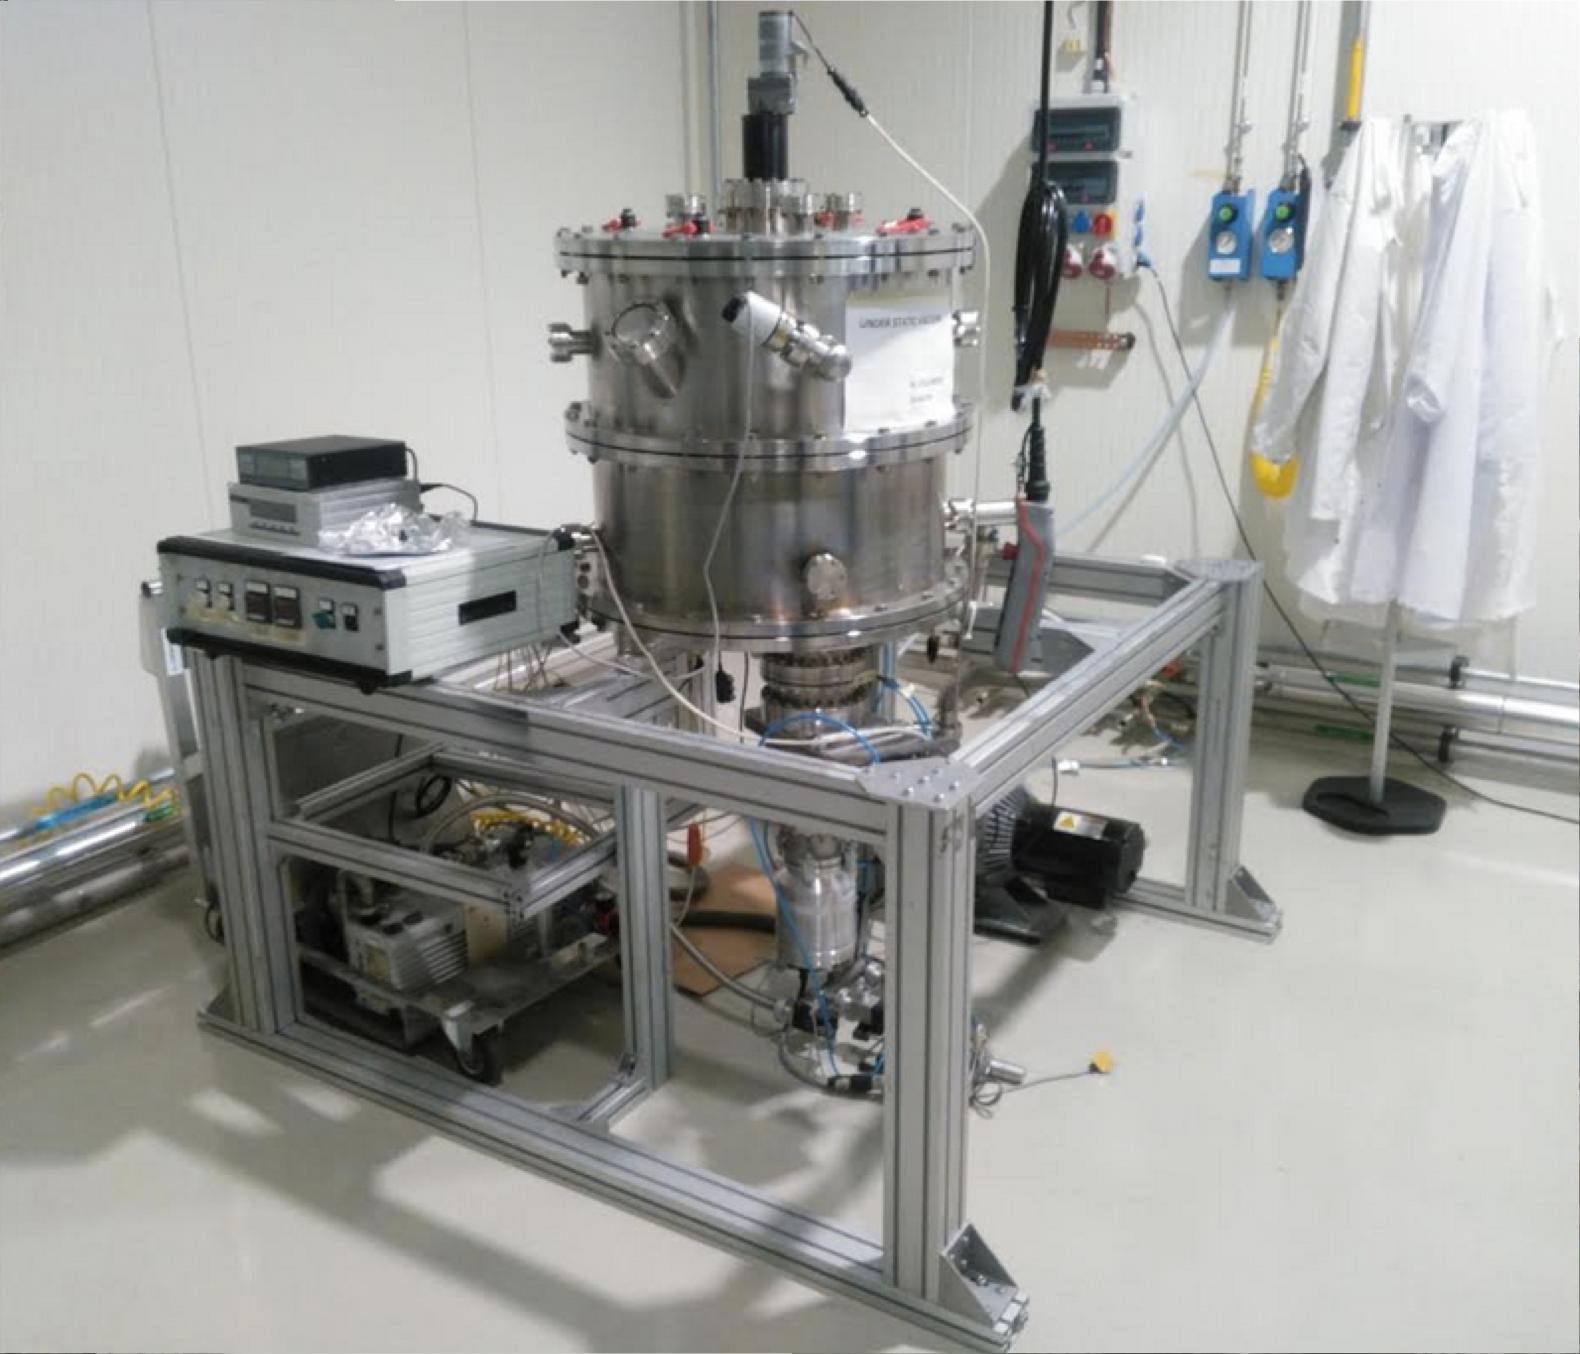
\includegraphics[height=8cm]{dppd_11_4_left.jpg}
\includegraphics[height=8cm]{dppd_11_4_right.jpg}
%\includegraphics[height=8cm]{dppd_11_4} too big
\end{dunefigure}

The \dwords{pmt} will be taken out of their individual cartons when they arrive at the \dword{ctsf}. The \dwords{pmt} will first be tested for basic functionality in their cartons to verify that they have been safely transported from the remote sites and will be kept in these boxes until the windows are coated. The \dword{pmt} windows will be cleaned with acetone and isopropanol before the evaporation. This will be done in the flow device/fume hood shown as a green box along the \SI{10}{\m} wall in Figure~\ref{fig:dppd_11_3}. The gantry crane (indicated with red bars in Figure~\ref{fig:dppd_11_3}) can move parts between the coating stations and the work desks. It will be used to remove the vessel lid and support it while the \dword{pmt} is installed for coating.

Following the evaporation procedure, acrylic protective plates will be installed to cover the coated \dword{pmt} windows.
%, and the \dwords{pmt} will be placed in individual dark plastic protective bags. 
The \dwords{pmt} will be tested again for basic functionality. They will then be attached to the \num{4} $\times$ \num{3} structure for transportation to \surf.

At the \dword{ctsf}, the \dword{pmt} windows will be coated at a rate of \num{4} \dwords{pmt}/day or \num{20} \dwords{pmt}/week and \num{80} \dwords{pmt}/month. Given the installation rate of \num{120} \dwords{pmt}/month, the \dword{ctsf} operations should start before installation begins. \dword{ctsf} has sufficient storage capacity for the entire \dword{pmt} inventory of the \dword{pds}. 

\subsection{Underground Installation and Integration}
\label{subsec:dp-pds-undergroundinstallation}

The cryostat cable/fiber installation will precede the installation of the \dword{fc}. The cables/fibers will be routed from the flanges to the bottom of the cryostat. The total cable/fiber mass (length) is approximately \SI{50}{\kg} (\SI{25}{\m}) per sector with an average mass/length of \SI{2}{\kg/\m}, where one sector comprises \num{36} \dwords{pmt} (see Section~\ref{sec:dp-pds-overview_layout}). The free ends of the cables/fibers will be temporarily attached to the cryostat floor so they can be easily accessed during installation. The cable/fiber and tray installation will be done on both sides of the cryostat. At this stage, the \dword{hv} cables will be transported in a single box from the \dword{ctsf} to \surf. At the same time, a separate box containing \num{120} calibration fiber + fiber bundle assemblies will be transported from the \dword{ctsf} to \surf. The boxes will be transported to the cryostat roof so the cables/fibers can be hung through the feedthroughs for installation in the cable trays.  

Once the plastic wrap is removed, the \dword{pds} \dword{pmt} box and its entire contents can be moved to the clean room. The \dwords{pmt} will undergo functionality tests inside the custom design dark box, which can cover the entire structure of \num{4} $\times$ \num{3} \dwords{pmt}. The dark box will have a high voltage patch panel and allow consecutive tests of all \num{12} \dwords{pmt} in one testing session without intervention. The test will be a simple check for healthy \dword{pmt} operations. Once the operation of the \dwords{pmt} is verified, the structure can be moved into the cryostat.

Inside the cryostat, the \dwords{pmt} will be removed from the structure. %The window protections will be kept on the \dwords{pmt}. 
The \dwords{pmt} will be mounted on the membrane floor in the areas between the membrane corrugations using their support structures. The attachment is done using a stainless steel support base that can be point-glued to the membrane. The weight of the support and the \dword{pmt} exceeds the buoyancy force of the system. Furthermore, these supports also ensure stability against possible lateral forces acting on the \dwords{pmt} due to the liquid flow. Once the attachment is complete, the short \dword{hv} cables will be connected to the cold \dword{hv} cables with SHV barrel connectors. The calibration fibers will be routed and connected to the support structure. Once all the \dwords{pmt} of a given \dword{pds} sector are installed, the cables and fibers will be fixed in their final positions.

The installation will be done at a rate of \num{30} \dwords{pmt}/week. After installation, the empty \dword{pmt} boxes and the transport structures will be taken back to \dword{ctsf}.

Table~\ref{tab:dppd_t_11_1} summarizes the quantities related to the \dual \dword{pds} installation.

\begin{dunetable}
[Quantities related to the \dual \dshort{pds} installation.]
{lc p{0.8\textwidth}}
{tab:dppd_t_11_1}
{Quantities related to the \dual \dword{pds} installation.}
Parameter & Value \\
Number of \dual \dword{pds} sectors	& \num{20} \\
Number of \dwords{pmt} per sector	& \num{36} \\
Number of calibration fibers per sector	& \num{6} \\
Number of feedthrough flanges per sector	& \num{1} \\
Total number of feedthrough flanges	& \num{20} \\
Number of \dword{hv} racks per sector	& \num{1} \\
Frequency of transportations to \surf from \dword{ctsf}	& \num{4} \dword{pds} boxes per month \\
Rate of installation	& \num{30} \dwords{pmt}/week \\
\end{dunetable}

The reflector/\dword{wls} panels will be assembled into a unit panel assembly on a dedicated table underground immediately prior to the installation following the procedure described in Section \ref{sec:dp-pds-mechanics}. They will be placed in a storage structure that can hold three regular and two extended reflector/\dword{wls} panel assemblies to be installed in one row of an \dword{fc} super-module. The installation of the panel assemblies will be synchronized with the installation of the \dword{fc} modules, which is described in Section \ref{sec:fddp-hv-transport-install} and depicted in Figure~\ref{fig:dp-super-module-installation-secuence}. Once a row of the \dword{fc} super-module is installed, the five reflector/\dword{wls} panel assemblies will be mounted on the FRP I-beams of the \dword{fc} submodules, starting from one end of the row and progressing towards the other. Figure \ref{fig:dppd_reflective_panel_installation_sequence} depicts the installation sequence of a unit reflector/\dword{wls} panel. The sequence can be described as below:

\begin{enumerate}
\item Put the top two screws accessing the back side through the top liquid flow opening (Figure~ \ref{fig:dppd_reflective_panel_installation_sequence}  left).
\item Place two nuts in the closed holes of the long holding bar. Slide the long bar behind the panel to the level of the middle bar by holding it through the central liquid flow opening. Put the two middle bar screws and remove the long bar through the bottom liquid flow opening after sliding it all the way down (Figure~ \ref{fig:dppd_reflective_panel_installation_sequence}  center).
\item Put the bottom two screws accessing the back side through the bottom liquid flow opening (Figure~ \ref{fig:dppd_reflective_panel_installation_sequence}  right).
\end{enumerate}

\begin{dunefigure}[Installation sequence of unit reflector/\dshort{wls} assembly on  \dshort{fc} I-beams]{fig:dppd_reflective_panel_installation_sequence}
{The schematic view of the installation sequence of a unit reflector/\dword{wls} panel assembly on the \dword{fc} I-beams: The installation of the top two screws (left), the middle two screws with the holding bar (center) and the bottom two screws (right). The I-beams are shown as blue vertical rectangles at each side of the panel assembly, the panels as grey squares and the horizontal support bars and the holding bar as green rectangles. The screw locations are indicated with red arrows.}
\includegraphics[width=0.8\textwidth]{dppd_reflective_panel_installation_sequence}
\end{dunefigure}

\subsection{Commissioning}
\label{subsec:dp-pds-commissioning}

The commissioning of the \dword{pds} is performed in partitions. The size of a single partition will be mainly determined by the \dword{daq} and the \dword{hv} systems. The \dword{daq} and \dword{hv} partitions are commissioned, including the relevant control systems, before the \dwords{pmt} are connected to these systems.

The exact availability of the cryostat as a sufficiently dark environment depends on the overall installation schedule. Once it is possible, the \dwords{pmt} are powered up, and basic functionality and performance checks are carried out. These include pedestal data taking, i.e., recording event data with external periodic triggering, and tests with the calibration system where the data taking is triggered in synchronization with a light source, as described in Section \ref{sec:dp-pds-calibration}.

Basic performance characteristics of the \dwords{pmt}, e.g., the dark count rate and gain, will be validated with the commissioning tests. Issues related to installation can then be identified and eliminated. A commissioned sector becomes a part of the overall detector and can join the global calibration data taking and commissioning.



\section{Risks}
\label{sec:dp-pds-risks}

Table~\ref{tab:dppd_t_12_1} shows the summary of the risks associated with the \dual \dword{pds}. Severity level assigned for each risk is indicated as L (low), M (medium) and H (high). Below, we discuss these risks and the mitigation plan for each risk item.

\begin{dunetable}
[Dual Phase Photon Detector Risk Summary]
{p{0.05\textwidth}p{0.7\textwidth}p{0.1\textwidth}}
{tab:dppd_t_12_1}
{Dual Phase Photon Detector Risk Summary.}
ID & Risk & Severity \\
1 & The photon detection system is not stable over the lifetime of the experiment (\dword{tpb}, channel) & L \\
2 & Implosion of \dwords{pmt} & L \\
3 & Fibers damaged during installation & L \\
4 & Background level (noise, light sources) is too high to distinguish signal & M \\
5 & \dword{pmt} signals are saturated & M \\
6 & Availability of resources for work at the installation/integration site is less than planned & M \\
7 & \dwords{pmt} damaged during shipment to the experiment site & M \\
8 & Not enough photons arriving to \dwords{pmt} & L \\
9 & Problems with choosing the correct type of screws and feedthroughs for the cabling and installation on the cryostat & M \\
10 & Excess noise due to poor grounding or not following grounding rules & M \\
11 & Problem with the connection of the cable to the \dword{pmt} base & L \\
12 & \dword{tpb} coating not sufficiently stable, contaminates \dword{lar} & L \\
\end{dunetable}

\begin{enumerate}

\item During the operation of the \dword{fd}, the photon detection system could show performance fluctuations. For example, the \dword{pmt} gains could change. Continuous monitoring with the \dword{pmt} calibration system will enable us to resolve these issues at the individual \dword{pmt} level.

\item A critical process could be the filling of the detector with \dword{lar} because a \dword{pmt} could implode. If this happens, the detector must be emptied. Special care must be taken during the filling of the detector with \dword{lar}. Pressure tests will be performed to quantify this.

\item Fibers are fragile and they could be broken during installation because of the high number of fibers in the detector. Special care during fiber installation must be taken by personnel in charge of the assembly of the different parts of the detector.

\item If external noise or light sources affect the \dwords{pmt}, it could be difficult to measure the signals without oscillations over the baseline. Grounding, shielding and power distribution are critical to the success of the experiment. Mitigation will be by using proper shielding techniques on all cables and validation of the noise performance of all equipment during the installation and commissioning phases.

\item If we have to increase the \dword{pmt} \dword{hv} in order to have higher gains, \dword{pmt} front-end inputs could be saturated. Then, we would loose a number of events in the acquisition. To mitigate this risk we will avoid to operate the \dwords{pmt} at very high voltages. A balance between gain and saturation will be chosen.

\item The \dword{fd} construction cost estimate assumes that qualified local labor can be identified for certain activities. The cost will increase if external labor is required. Labor costs might need to increase to attract qualified candidates. Labor resources from laboratories may need to be housed and used. We will ensure that sufficient funding is available to move people temporarily from institutions involved in the \dword{pds} consortium to the integration/installation site.

\item If \dwords{pmt} are not packaged properly, they could be damaged during shipment. In this case, the \dword{pmt} cannot be used in the detector. We will use special packaging to avoid possible damages to the \dwords{pmt} during shipment. In any case, we will have a \num{10} \% contingency spare \dwords{pmt}.

\item Due to the long drift distance and the position of the cathode and the ground grid on top of the \dwords{pmt}, the number of photons reaching the \dwords{pmt} might not be sufficient at some geometrical acceptances. Additional light collection enhancement tools are being considered to mitigate this effect. The most feasible option is the installation of a wavelength shifting film on the inner surface of the field cage.

\item Choosing a wrong feedthrough means we could have a higher noise level or oscillations in the signals. Wrong parts might cause mechanical problems. Special care must be taken during the design of the screws and \dword{hv} feedthroughs needed for cabling in the detector. \dword{pddp} experience will be employed to mitigate this risk.

\item During commissioning of the detector prior to \dword{lar} filling, it could be observed that an excessive noise appears due to some components failing to fulfill the grounding rules. We will ensure that grounding rules are enforced and review any proposed modification of the detector design.

\item \dword{pmt} cables are soldered to the \dword{pmt} base and tested before installation. In case of a bad soldering, some channels could show a bad waveform or no signal. Several tests will be done in the base before the installation of the \dword{pmt}: impedance, \dword{hv} tests in gas Ar to avoid sparks and full test of the \dword{pmt} to verify the signals are correct.

\item Limited past experience demonstrates that the \dword{tpb} coating might not be sufficiently stable and can contaminate the \dword{lar} in the long term. We will carefully examine results from \dword{pddp} and other laboratory tests% as quickly as possible
. We will elaborate improved coating techniques if needed.

\end{enumerate}
\section{Safety}
\label{sec:fddp-pds-safety}



\section{Project Management}
\label{sec:dp-pds-management}

The \dual \dword{pd} consortium was formed in 2017;  it comprises eleven institutions from France, Peru, Spain, UK, and USA. The charge of the \dual \dword{pd} consortium is to plan and execute the construction, installation, and commissioning of the \dual \dword{pds}.
% I think we should check with Peru and UK if they are still interested in being included in the consortium

%%%%%%%%%%%%%%%%%%%%%%%%%%%%%%%%%
\subsection{Consortium Organization}

The current \dual \dword{pd} consortium leader is %In\'{e}s Gil-Botella
 from CIEMAT (Spain) and the technical lead is %Dominique Duchesneau 
 from LAPP (France). They are members of the \dword{dune} technical board and represent the consortium in the overall \dword{dune} collaboration. The consortium leader is responsible for the subsystem deliverables and for effectively managing the consortium. The technical lead acts as the overall project manager and is the interface to the international project office; he is responsible for monitoring and reporting on progress on the agreed schedule and for interface documentation.

The institutions participating in the consortium are responsible for the design and/or construction of a particular subsystem. The national groups within the consortium plan to approach relevant funding agencies with a specific construction-phase proposal to obtain a likely funding line in 2019. The \dual \dword{pd} consortium is open to any new institution willing to join the current effort.

The current institutions participating in the \dual \dword{pd} consortium are LAPP (France); PUCP (Peru); IFAE, CIEMAT, and IFIC (Spain); UCL (UK); and ANL, Duke U., U. of Iowa, SDSMT, and UTA (USA).

The \dual \dword{pd} consortium is divided into four working groups: photosensors and electronics; calibration system; mechanics and integration; and simulation and physics. The corresponding current Working Group convener institutions are
\begin{itemize}
% AH REMOVING NAMES
\item WG1: Photosensors and Electronics -  CIEMAT, %A. Verdugo
\item WG2: Calibration System -  CIEMAT, %C. Cuesta
\item WG3: Mechanics and Integration - University of Iowa%, and %B. Bilki 
\item WG4: Simulation and Physics - %K. Scholberg (
Duke University, %M. Sorel (
IFIC, %L. Zambelli (
LAPP.
\end{itemize}

%%%%%%%%%%%%%%%%%%%%%%%%%%%%%%%%%
%\subsection{Planning Assumptions}
%\label{sec:fddp-pd-12.2}

%The optimization and final design of the \dual \dword{pd} system will be driven by the \dword{pddp} data, expected by Summer 2019.

%\dword{pddp} operation and data analysis are fundamental steps to understanding whether the current \dword{pds} design considered as baseline, based on cryogenic \dwords{pmt} with \dword{tpb} coating, is able to provide $t_0$ for non-beam events, background rejection and triggering on non-beam events. These data will be used to tune the \dword{mc} simulations and extrapolate the performance of the system to the \dword{dpmod}.


\subsection{Planning Assumptions}
\label{sec:fddp-pd-12.2}

The baseline design of the \dual \dword{pds} is a complex optimization based on the results from and experience with the first tonne scale dual phase \dword{lar} \dword{tpc} demonstrator (\dword{wa105}), critical evaluation of the design and construction of \dword{wa105} and \dword{pddp}, physics objectives of the \dune experiment, and the detailed simulation studies of \dune \dword{dp} as well as \dword{wa105} and \dword{pddp}.

The previous design and construction of the \dual modules have enabled us to critically evaluate several scenarios and develop the \dune \dword{pds} design optimized for maximum physics performance; simple construction, transportation, handling, and installation; and easy and robust operation.

Simulations are effectively used in designing and optimizing the \dual \dword{pd} system to meet the physics requirements:
\begin{itemize}
\item light collection efficiency,
\item number of channels,
\item photosensor requirements,
\item dynamic range of readout electronics and timing resolution, and 
\item trigger strategy on non-beam events.
\end{itemize}

Although no major design modifications are foreseen, the \dword{pddp} operations will be closely monitored to fine-tune the \dune \dual design.

%%%%%%%%%%%%%%%%%%%%%%%%%%%%%%%%%
%\subsection{\dword{wbs} and Institutional Responsibilities}
\subsection{Work Breakdown Structure and Institutional Responsibilities}

The \dual \dword{pd} consortium has developed a detailed breakdown of deliverables and responsibilities \citedocdb{5606} included in the overall \dword{dune} collaboration \dword{wbs} \citedocdb{5594}%\cite{bib:docdb5594} 
coordinated by the international project office. The main deliverables are %based on the \dword{pddp} \dword{pds}  and are 
divided into seven topics: 
%These are listed along with the participating institutions below: 

%\dword{pddp} \dword{pds} 
\begin{enumerate}
\item Management \dual \dword{pds} (includes milestones and review dates),
\item Physics and simulations,
\item Design, engineering, R\&D, and validation tests,
\item Production set up (includes tooling),
\item Production (includes component production, assembly, testing, and \dword{qc}),
\item Integration (contributions to activities at global integration facility), and
\item Installation (contributions to activities at \surf).

%\item Management \dual \dword{pds} (includes milestones and review dates) \textit{- LAPP, CIEMAT }
%\item Physics and Simulations \textit{- Duke, LAPP, IFIC, SDSMT, CIEMAT, PUCP, UCL, Texas-Austin}
%\item Design, Engineering, R\&D and validation tests \textit{- Iowa, CIEMAT, IFIC, UCL, Texas-Austin, IFAE, SDSMT}
%\item Production Setup (includes tooling) \textit{- UCL}
%\item Production (includes component production, assembly, testing, and \dword{qc}) \textit{- Iowa, CIEMAT, IFAE, IFIC, UCL, Texas-Austin, Duke, SDSMT, LAPP}
%\item Integration (contributions to activities at global integration facility) \textit{- SDSMT}
%\item Installation (contributions to activities at \surf) \textit{- CIEMAT, IFIC, SDSMT, Iowa}
\end{enumerate}

\subsection{High Level Schedule}

%\fixme{Table~\ref{tab:Xsched} is a standard table template for the TDR schedules.  It contains overall FD dates from Eric James as of March 2019 (orange) that are held in macros in the common/defs.tex file so that the TDR team can change them if needed. Please do not edit these lines! Please add your milestone dates to fit in with the overall FD schedule. Please set captions and label appropriately. Anne}

The main high-level milestones of the \dual \dword{pds} and the dates by which they will be accomplished are summarized in Table~\ref{tab:Xsched}.

\begin{dunetable}
[\dual \dword{pd} Consortium Schedule]
{p{0.65\textwidth}p{0.25\textwidth}}
{tab:Xsched}
{\dual \dword{pd} Consortium Schedule}   
Milestone & Date (Month YYYY)   \\ \toprowrule
%Technology Decision Dates &      \\ \colhline
%Final Design Review Dates &      \\ \colhline
%Start of module 0 component production for ProtoDUNE-II &      \\ \colhline
%End of module 0 component production for ProtoDUNE-II &      \\ \colhline
\rowcolor{dunepeach} Start of \dword{pdsp}-II installation& \startpduneiispinstall      \\ \colhline
\rowcolor{dunepeach} Start of \dword{pddp}-II installation& \startpduneiidpinstall      \\ \colhline
% \dword{prr} dates &      \\ \colhline
%Start of  (component 1) production  &      \\ \colhline
%Start of (component 2) production  &      \\ \colhline
%Start of  (component 3) production  &      \\ \colhline
\rowcolor{dunepeach}South Dakota Logistics Warehouse available& \sdlwavailable      \\ \colhline
\rowcolor{dunepeach}Beneficial occupancy of cavern 1 and \dword{cuc}& \cucbenocc      \\ \colhline
\rowcolor{dunepeach} \dword{cuc} counting room accessible& \accesscuccountrm      \\ \colhline


\rowcolor{dunepeach}Top of \dword{detmodule} \#1 cryostat accessible& \accesstopfirstcryo      \\ \colhline

\dword{pmt} procurement procedure and production & June 2024 \\ \colhline
\dword{pmt} base design and manufacturing &  June 2024 \\ \colhline
\dword{pmt} support structure production and assembly & July 2024 \\ \colhline


%End of  (component 1) production  &      \\ \colhline
%... & ...                       \\ \colhline

\rowcolor{dunepeach}Start of \dword{detmodule} \#1 TPC installation& \startfirsttpcinstall      \\ \colhline

\rowcolor{dunepeach}End of \dword{detmodule} \#1 TPC installation& \firsttpcinstallend      \\ \colhline

\rowcolor{dunepeach}Top of \dword{detmodule} \#2 accessible& \accesstopsecondcryo      \\ \colhline

\dword{pmt} characterization & April 2025 \\ \colhline
Fibers, light source tests and procurement & April 2025 \\ \colhline
Splitter production and tests & June 2025 \\ \colhline
\dword{tpb} coating of the \dwords{pmt} & July 2025 \\ \colhline
\dword{tpb} coating of the reflector/\dword{wls} panels & July 2025 \\ \colhline

 \rowcolor{dunepeach}Start of \dword{detmodule} \#2 TPC installation& \startsecondtpcinstall      \\ \colhline
 
\dword{pmt} cable and fiber routing in cryostat from flange to bottom & October 2025 \\ \colhline
\dword{pmt} testing, installation in cryostat and cabling & April 2026 \\ \colhline
\dword{pmt} support installation on the membrane & April 2026 \\ \colhline
Splitter installation & April 2026 \\ \colhline
Fiber calibration system installation & April 2026 \\ 
 
\rowcolor{dunepeach}End of \dword{detmodule} \#2 TPC installation& \secondtpcinstallend      \\ 

%last item & ...                         \\
\end{dunetable}



%The \dual \dword{pds} consortium's main activities during the next \num{16} months are focused on developing the \dword{tdr}. 
%The main high-level milestones are detailed in Table~\ref{tab:dppd_t_12_5} for the pre-\dword{tdr} period. The plan for the activities in the post-\dword{tdr} period is summarized in Table~\ref{tab:dppd_t_12_6}.

%The main high-level milestones for the pre-installation are summarized in Table~\ref{tab:dppd_t_12_n1} and installation periods in  Table~\ref{tab:dppd_t_12_n2}. The installation period schedule is expressed as the start month and the end month with respect to the start of installation of the \dune \dual.

%\begin{dunetable}
%[Pre-\dword{tdr} key milestones]
%{|l|l| p{0.8\textwidth}}
%{tab:dppd_t_12_5}
%{Pre-\dword{tdr} key milestones (TO BE UPDATED)}

%Milestone & End date \\ \toprowrule
%Simulations and physics: %Finalize the 
%Implementation of \dual optical & \\
%simulation in \larsoft for \dword{pddp} & 08/2018 \\ \colhline
%Simulations and physics: Optimization of the & \\
%\dword{dpmod} performance to fulfill the physics requirements and & \\
%definition of a trigger strategy & 05/2019 \\ \colhline
%Photosensors: Components selection and final design & 03/2019 \\ %\colhline
%\dword{pmt} calibration system design and selection of components & 03/2019 \\ \colhline
%Cabling definition and design of flange & 03/2019 \\ \colhline
%Design review in light of \dword{pddp} calibration data & 03/2019 \\ %\colhline
%\dword{qc} plan & 06/2018 \\ \colhline
%Identification of Interfaces & 06/2018 \\ \colhline
%Integration, installation and commissioning plans & 12/2018 \\ \colhline
%\dword{dpmod} \dword{tdr} & 06/2019 \\ 
%\end{dunetable}

%\fixme{Remove table with pre-TDR milestones, Tab.~\ref{tab:dppd_t_12_5}?}

%\begin{dunetable}
%[Post-\dword{tdr} key milestones]
%{|l|l|l| p{0.8\textwidth}}
%{tab:dppd_t_12_6}
%{Post-\dword{tdr} key milestones}

%Milestone & Start date & End date \\ \toprowrule
%\textbf{\dword{pmt} preparation and installation} (can be done in batches) & & \\ \colhline
%\dword{pmt} procurement procedure and production & 01/2021 & 12/2022 \\ %\colhline
%\dword{pmt} base design and manufacturing & 01/2022 & 12/2022 \\ %\colhline
%\dword{pmt} support structure production and assembly & 08/2022 & 01/2023 \\ \colhline
%\dword{pmt} characterization - \num{10} \dwords{pmt}/week (two facilities) & 02/2023 & 12/2023 \\ \colhline
%\dword{tpb} coating (two facilities similar to that for CERN ICARUS) & 01/2024 & 12/2024 \\ \colhline
%Splitter production and tests & 05/2024 & 12/2024 \\ \colhline
%\textbf{Installation at \surf} & & \\ \colhline
%\dword{pmt} cable and fiber routing in cryostat from flange to bottom & & \\
%                  (depends on \dword{fc} and flange installation) & 09/2024 & 09/2024 \\ \colhline
%\dword{pmt} testing, installation in cryostat and cabling (\num{72} %\dwords{pmt}/month) & 10/2024 & 07/2025 \\ \colhline
%\dword{pmt} support installation on the membrane & & \\
%                  (in parallel by sector with \dword{pmt} installation) & 10/2024 & 07/2025 \\ \colhline
%Splitter installation & & \\
%                  (in parallel with \dword{pmt} installation to test cabling and connections) & 10/2024 & 07/2025 \\ \colhline
%\textbf{Light calibration system} & & \\ \colhline
%Fibers, light source tests and procurement & 06/2023 & 05/2024 \\ %\colhline
%Fiber calibration system installation & & \\
%                  (in parallel with \dword{pmt} installation with validation test) & 09/2024 & 07/2025 \\ 
%\end{dunetable}



%\begin{dunetable}
%[Pre-Installation Period Key Milestones]
%{|l|l|l| p{0.8\textwidth}}
%{tab:dppd_t_12_n1}
%{Pre-Installation Period Key Milestones.}
%
%Milestone & Start date & End date \\ \toprowrule
%\textbf{\dword{pmt} preparation and installation} (can be done in batches) & & \\ \colhline
%\dword{pmt} procurement procedure and production & 01/2021 & 12/2022 \\ \colhline
%\dword{pmt} base design and manufacturing & 01/2022 & 12/2022 \\ \colhline
%\dword{pmt} support structure production and assembly & 08/2022 & 01/2023 \\ \colhline
%\dword{pmt} characterization - \num{10} \dwords{pmt}/week (two facilities) & 02/2023 & 12/2023 \\ \colhline
%\dword{tpb} coating (two facilities similar to that for CERN ICARUS) & 01/2024 & 12/2024 \\ \colhline
%Splitter production and tests & 05/2024 & 12/2024 \\ \colhline
%\textbf{Light calibration system} & & \\ \colhline
%Fibers, light source tests and procurement & 06/2023 & 05/2024 \\ \colhline
%\end{dunetable}

%\begin{dunetable}
%[Installation Period Key Milestones]
%{|l|c|c| p{0.8\textwidth}}
%{tab:dppd_t_12_n2}
%{Installation Period Key Milestones.}
%
%Milestone & Start month & End month \\ \toprowrule
%\dword{pmt} cable and fiber routing in cryostat from flange to bottom & & \\
%                  (depends on \dword{fc} and flange installation) & 1 & 2 \\ \colhline
%\dword{pmt} testing, installation in cryostat and cabling (\num{120} \dwords{pmt}/month) & 2 & 8 \\ \colhline
%\dword{pmt} support installation on the membrane & & \\
%                  (in parallel by sector with \dword{pmt} installation) & 2 & 8 \\ \colhline
%Splitter installation & & \\
%                  (in parallel with \dword{pmt} installation to test cabling and connections) & 2 & 8 \\ \colhline
%Fiber calibration system installation & & \\
%                  (in parallel with \dword{pmt} installation with validation test) & 2 & 8 \\ 
%\end{dunetable}


%\fixme{Update Tab.~\ref{tab:dppd_t_12_6} according to new schedule, with installation of 2nd module starting on 08/2025.}

\subsection{High Level Cost of Baseline Design}


%\fixme{I just added the new template -- the autogeneration is not yet in place, so this is the best place to start. 4/4/19. Anne}

An initial cost estimate of the \dword{pds} for one \SI{10}{kt} \dword{dune} \dword{dpmod} was developed and presented in Table~\ref{tab:dp-pds-costsumm}. This is based on \dword{pddp} costs.
 
\begin{dunetable}
[\dual \dword{pds} Cost Summary]
{p{0.5\textwidth}p{0.2\textwidth}p{0.2\textwidth}}
{tab:dp-pds-costsumm}
{\dual \dword{pds} Cost Summary (TO BE COMPLETED)}   
Cost Item & M\&S (k\$ US) & Labor Hours \\ \toprowrule

Project Management &     &             \\ \colhline
Physics and Simulations &     &             \\ \colhline

\rowcolor{dunepeach} Design, Engineering and R\&D &  &     \\ \colhline
 Photosensors &     &             \\ \colhline
 Mechanics &     &             \\ \colhline
 Electronics, Cables and \dword{hv} &     &             \\ \colhline
 Calibration System &     &             \\ \colhline
 Integration and Installation &     &             \\ \colhline
 \rowcolor{dunepeach} Production Setup &  &     \\ \colhline
 Photosensors  &     &             \\ \colhline
 Mechanics &     &             \\ \colhline 
 Electronics, Cables and \dword{hv} &     &             \\ \colhline
 Calibration System &     &             \\ \colhline 
 Integration and Installation &     &             \\ \colhline
\rowcolor{dunepeach} Production &  &     \\ \colhline
 Photosensors  &     &             \\ \colhline
 Mechanics &     &             \\ \colhline 
 Electronics, Cables and \dword{hv} &     &             \\ \colhline
 Calibration System &     &             \\ \colhline 
 Integration and Installation &     &             \\ \colhline
\rowcolor{dunepeach} DUNE FD Integration \& Installation  &  &     \\ %\colhline
%\dword{pmt} Testing at \dword{ctsf} &     &             \\ \colhline
%\dword{wls} Production &     &             \\ \colhline
%\dword{wls} Testing &     &             \\ \colhline

%Signal/Optical Flanges Installation &     &             \\ \colhline
%\dword{pmt} Installation &     &             \\ \colhline
%\dword{pmt} Cabling and Optical Fibers to Feedthrough  &     &             \\ \colhline
%Cabling from Feedthrough to Splitter  &     &             \\ \colhline
%Cabling from Splitter to \dword{hv} Power Supply &     &             \\ \colhline
%Cabling from Splitter to \dword{utca} \dword{fe} Electronics &     &             \\ \colhline
%Light Electronic Rack Installation &     &             \\ \colhline
%Installation Tests &     &             \\ \colhline
%Commissioning &     &             \\ \colhline

\end{dunetable}
\newpage

\section{Appendix - Alternatives}
\label{sec:dp-pds-appendix}

\subsection{Individual Ground Grids}
\label{sec:dp-pds-appendix-grid}

In collaboration with the \dword{hv} consortium, the installation of individual ground grids for each \dword{pmt} in place of the ground grid table structure is under consideration. Since the individual ground grid cages will potentially have thinner wires and will be closer to the \dword{pmt} windows, generating a smaller shadow, they should increase the acceptance of the \dwords{pmt}.

The feasibility of the design in operation under \dune \dual conditions will be studied by the \dword{hv} consortium. The design of the individual grids will be developed as a common effort of the two consortia engineering teams. The \dword{hv} consortium will produce the grids. The grids will be installed at the \dword{ctsf} by \dual \dword{pd} consortium. The \dwords{pmt} will be installed with their individual grid cages by \dual \dword{pd} consortium. 

\subsection{Calibration System Alternatives}
\label{sec:dp-pds-appendix-calibration}

Alternatives to the baseline design of the calibration system described in Section~\ref{sec:dp-pds-calibration} will be pursued with R\&D measurements to make the system more effective, reduce the cost, and mitigate issues related to scaling to the \dune \dual size. These alternatives include reducing the number of fibers, studying other options for the reference sensor, and increasing the input light if necessary. To reduce the number of fibers, light diffusers can be used, so that one fiber can illuminate at least four \dwords{pmt}. For instance, a diffuser could be placed at the ground grid, or in the case of individual ground grids, on the side walls. With the same aim of reducing the total number of fibers, an alternative calibration system with two fibers placed at the top of the field cage is being tested in \dword{pddp}, so that one fiber can illuminate several \dwords{pmt}. Other than the diffusers and fiber placement, considered alternatives are related to the external system and can be implemented with minimal interference with other subsystems.

\subsection{Xe Doping of Liquid Argon}
\label{sec:dp-pds-appendix-xedoping}

Doping the \dword{lar} volume with Xe is an attractive option in terms of providing a volume distributed wavelength shifting. Major advantages of Xe doping are triggering the long-lived triplet argon excimer to produce a faster signal reducing the fraction of late light; shifting the scintillation signal to longer wavelengths (\SI{175}{nm}) and as a consequence, a longer Rayleigh scattering length.

Dedicated simulations on light yield in the full \dword{dp} \dword{fd} cryostat in the presence of Xe doping were performed. Figure~\ref{fig:dppd_fd_light_yield_xedoping} shows the 1D light yields as a function of the drift (transverse) direction in the left (right) panel, averaging over the other two spatial coordinates. It is evident that the Xe doping can be considered as an immediate alternative to the baseline design with half coverage reflector/\dword{wls} panels in terms of light output. On the other hand, keeping a smaller area coverage reflector/\dword{wls} panels closer to the charge readout may be preferable in order to improve the uniformity.

%\subsection{Wavelength Shifting Reflective Foils}
%\label{sec:dp-pds-appendix-wlsfoils}

%To enhance light collection and improve response uniformity in the detector volume, installing wavelength shifting reflector foils on the \dword{fc} inner surfaces is under consideration. This alternative is being evaluated for two particular cases: covering \dword{fc} inner walls fully with the foils and covering only the upper half of the \dword{fc} with the foils. In addition to completely evaluating the effect on physics within the consortium, the interface, particularly the effect on liquid circulation, the effective electric field, and the mechanical structure are being discussed with the \dword{hv} consortium.

%\fixme{If included in the baseline design, move to section \ref{sec:dp-pds-mechanics}}

\begin{dunefigure}[Expected 1D light yields in the full \dshort{dpmod} with xenon doping]{fig:dppd_fd_light_yield_xedoping}
{Expected light yield in the full \dword{dp} \dword{fd} cryostat in the presence of xenon doping. The yield units are number of photo-electrons per \si{\MeV} of deposited energy. The 1D yields are shown as a function of the drift (transverse) direction in the left (right) panel, averaging over the other two spatial coordinates (not shown), similarly to Figure~\ref{fig:dppd_fd_light_yield_comparisons}. The three histograms correspond to the half foil baseline design without xenon doping, and to two no foil geometries, with and without xenon doping, respectively.}
\raisebox{0.1cm}{\includegraphics[width=0.49\textwidth]{graphics/dppd_xedoping_drift.png}} \hfill
\includegraphics[width=0.49\textwidth]{graphics/dppd_xedoping_transverse.png}
\end{dunefigure}